\documentclass[oneside, a4paper,11pt]{book}
\usepackage{graphicx}
\usepackage{wrapfig}
\usepackage{verbatim}
\usepackage{fancyhdr}
\usepackage{url}
\usepackage{supertabular}
\usepackage{multicol}
\usepackage{setspace}

\usepackage{array}
\usepackage{colortbl}

\usepackage{amsmath}
\usepackage{amsthm}
\usepackage{amssymb}
\usepackage{cancel}
\usepackage{mathtools}
\usepackage{extpfeil}
%\usepackage[only, llbracket, rrbracket]{stmaryrd}


\usepackage[pagebackref=false]{hyperref}
\usepackage[rgb,x11names,dvipsnames]{xcolor}% Optimize for screen reading.
\usepackage{longtable}
\usepackage{listings}
\lstdefinelanguage{scala}{
  morekeywords={import, object, class, case, var, val, if, else, while, for, from, to, extends, def, self, false, true, now, loop, react, ruturn, override},
  otherkeywords={=>,<-,::},
  sensitive=true,
  morecomment=[l]{//},
  morecomment=[n]{/*}{*/},
  morestring=[b]",
  morestring=[b]',
  morestring=[b]"""
}

\lstset{frame=tb,
  language=scala,
  aboveskip=0mm,
  belowskip=0mm,
  showstringspaces=false,
  columns=flexible,
  basicstyle={\small\ttfamily},
  keywordstyle=\color{RedViolet},
  numbers=left,
  numberstyle=\tiny\color{blue},
  numbersep=5pt,
  stringstyle=\color{Dandelion},
  stepnumber=1,
  frame=none,
  breaklines=true,
  breakatwhitespace=true,
  tabsize=2
  float=[hptb]
}
\usepackage[xindy]{glossaries}
\usepackage[margin=10mm,font={footnotesize},labelfont={footnotesize}]{caption}
\usepackage[section]{placeins}
\usepackage{xepersian}

\hypersetup{
   colorlinks,%
   filecolor=black,%
   linkcolor=DeepSkyBlue4,
  urlcolor=Chocolate4,
  citecolor=Cyan4,
    bookmarks=true,         
  %  unicode=true,          
    pdfstartview={FitH},    
    pdftitle={Design of Domain Using Asynchronous Message Passing},    
    pdfsubject={طراحی منطق دامنه بر اساس تبادل ناهمگام پیغام}
    pdfauthor={وحید ذوقی},  
    pdfsubject={پایان‌نامه‌ی کارشناسی ارشد},  
    pdfcreator={Vahid Zoghi},   
    pdfkeywords={Asynchronous Message Passing, Domain Modeling, Concurrency, Design Patterns}, 
}

\numberwithin{equation}{chapter}
\numberwithin{table}{chapter}
\numberwithin{figure}{chapter}
\numberwithin{equation}{chapter}

\settextfont[Scale=1.2]{XB Niloofar}
\setlatintextfont[Scale=1.2]{Times New Roman}
\DeclareMathSizes{10}{12}{8}{6}   % For size 10 text
\defpersianfont\shafigh[Scale=1]{Times New Roman}


\linespread{2}
\setlength\parskip{0.25cm}
\setlength\topmargin{-0.5in}
\setlength\headheight{2cm}
\setlength\headsep{0.7cm}
\setlength\textheight{8.8in}
\setlength\textwidth{6.5in}
\setlength\oddsidemargin{-0.3in}
\setlength\evensidemargin{0.0in}


\newenvironment{strict_enumerate}
{\begin{enumerate}
  \setlength{\itemsep}{1pt}
  \setlength{\parskip}{0pt}
  \setlength{\parsep}{0pt}}
{\end{enumerate}}

\newenvironment{strict_itemize}
{\begin{itemize}
  \setlength{\itemsep}{6pt}
  \setlength{\parskip}{0pt}
  \setlength{\parsep}{0pt}}
{\end{itemize}}


\newenvironment{strict_description}
{\begin{description}
  \setlength{\itemsep}{6pt}
  \setlength{\parskip}{0pt}
  \setlength{\parsep}{0pt}}
{\end{description}}

\newtheorem{definition}{تعریف}[chapter]
\newtheorem*{definition*}{تعریف}
\newtheorem{algorithm}{الگوریتم}[chapter]
\newtheorem{theorem}{قضیه}[chapter]
\newtheorem{lemma}{لم}[chapter]

%\let\lstinputlistingO=\lstinputlisting
\newcommand{\codelisting}[4][]
{
\begin{figure*}
\begin{latin}
\begin{center}
\begin{tabular}[hbtp]{c}

\linespread{1.4}
\lstinputlisting[#1]{#2}

\end{tabular}
\end{center}
\end{latin}
\caption{#3}
\label{#4}
\end{figure*}
}
%\newcommand{\codelstinputlisting}[2]{
%\begin{latin}
%linespread{6}
%\lstinputlisting[{#1}]{{#2}}
%\end{latin}
%}




\newglossarystyle{mylist}{%
% put the glossary in the itemize environment:
\renewenvironment{theglossary}{}{}%
% have nothing after \begin{theglossary}:
\renewcommand*{\glossaryheader}{}%
% have nothing between glossary groups:
\renewcommand*{\glsgroupheading}[1]{}%
\renewcommand*{\glsgroupskip}{}%
% set how each entry should appear:
\renewcommand*{\glossaryentryfield}[5]{%
%\item[] % bullet point
\glstarget{##1}{##2}% the entry name
\dotfill% the symbol in brackets
\space ##3 \\% the number list in square brackets
}%
% set how sub-entries appear:
\renewcommand*{\glossarysubentryfield}[6]{%
\glossaryentryfield{##2}{##3}{##4}{##5}{##6}}%
}

\makeglossaries
\newglossaryentry{بازیگر}{name={بازیگر}, description={\lr{Actor}}}
\newglossaryentry{مدل بازیگر}{name={مدل بازیگر}, description={\lr{Actor Model}}}
\newglossaryentry{لفافه‌بندی‌شده}{name={لفافه‌بندی‌شده}, description={\lr{Encapsulated}}}
\newglossaryentry{رفتار}{name={رفتار}, description={\lr{Behavior}}}
\newglossaryentry{تجزیه‌ناپذیر}{name={تجزیه‌ناپذیر}, description={\lr{Atomic}}}
\newglossaryentry{انصاف}{name={انصاف}, description={\lr{Fairness}}}
\newglossaryentry{حالت}{name={حالت}, description={\lr{State}}}
\newglossaryentry{حالت مشترک}{name={حالت مشترک}, description={\lr{Shared State}}}
\newglossaryentry{تجزیه}{name={تجزیه}, description={\lr{Decomposition}}}
\newglossaryentry{شیءگونه}{name={شیءگونه}, description={\lr{Object-Style}}}
\newglossaryentry{شیء-بنیاد}{name={شیء-بنیان}, description={\lr{Object-Based}}}
\newglossaryentry{استدلال}{name={استدلال}, description={\lr{Reason}}}
\newglossaryentry{بی‌قاعده}{name={بی‌قاعده}, description={\lr{Irregular}}}
\newglossaryentry{مقیاس‌پذیر}{name={مقیاس‌پذیر}, description={\lr{Scalable}}}
\newglossaryentry{پراکنده}{name={پراکنده}, description={\lr{Sparse}}}
\newglossaryentry{حالت محلی}{name={حالت محلی}, description={\lr{Local State}}}
\newglossaryentry{واکنشی}{name={واکنشی}, description={\lr{Reactive}}}
\newglossaryentry{همگام}{name={همگام}, description={\lr{Synchronous}}}
\newglossaryentry{ناهمگام}{name={ناهمگام}, description={\lr{Asynchronous}}}
\newglossaryentry{شی‌ء}{name={شی‌ء}, description={\lr{Object}}}
\newglossaryentry{ریسمان}{name={ریسمان}, description={\lr{Thread}}}
\newglossaryentry{میانگیری‌شده}{name={میانگیری‌شده}, description={\lr{Buffered}}}
\newglossaryentry{زمان‌بندی}{name={زمان‌بندی}, description={\lr{Scheduling}}}
\newglossaryentry{ارلانگ}{name={ارلانگ}, description={\lr{Erlang}}}
\newglossaryentry{بررسی گونه‌ها}{name={بررسی گونه‌ها}, description={\lr{type checking}}}
\newglossaryentry{مشخصه}{name={مشخصه}, plural={مشخصات},description={\lr{property}}}
\newglossaryentry{پیاده‌سازی}{name={پیاده‌سازی}, description={\lr{implementation}}}
\newglossaryentry{گونه}{name={گونه}, description={\lr{type}}}
\newglossaryentry{میان‌گذاری}{name={میان‌گذاری}, description={\lr{interleaving}}}
\newglossaryentry{همروند}{name={همروند}, description={\lr{Concurrent}}}
\newglossaryentry{غیرقطعی}{name={غیرقطعی}, description={\lr{Non-deterministic, Indeterminate}}}
\newglossaryentry{رده}{name={رده}, description={\lr{category}}}
\newglossaryentry{گزینه}{name={گزینه}, description={\lr{choice}}}
\newglossaryentry{درخت‌ طبقه‌بندی}{name={درخت‌ طبقه‌بندی}, description={\lr{classification tree}}}
\newglossaryentry{مورد کاربرد}{name={مورد کاربرد}, description={\lr{use case}}, plural={موارد کاربرد}}
\newglossaryentry{بسته‌}{name={بسته‌}, description={\lr{package}}}
\newglossaryentry{رویداد}{name={رویداد}, description={\lr{event}}}
\newglossaryentry{حوزه‌}{name={حوزه‌}, description={\lr{scope}}}
\newglossaryentry{بازه}{name={بازه}, description={\lr{range}}}
\newglossaryentry{نمونه}{name={نمونه}, description={\lr{instance}}}
\newglossaryentry{کنش}{name={کنش}, description={\lr{action}}}
\newglossaryentry{ناحیه}{name={ناحیه}, description={\lr{region}}}
\newglossaryentry{بازمتن}{name={متن‌باز}, description={\lr{open source}}}
\newglossaryentry{مطابقت}{name={مطابقت}, description={\lr{conformance}}}
\newglossaryentry{تراکنش‌}{name={تراکنش‌}, description={\lr{transaction}}}
\newglossaryentry{منطق دامنه}{name={منطق دامنه}, description={\lr{domain logic}}}
\newglossaryentry{آزمون واحد}{name={آزمون واحد}, description={\lr{unit test}}}
\newglossaryentry{خاص-دامنه}{name={خاص-دامنه}, description={\lr{domain specific}}}
\newglossaryentry{یک‌پارچه}{name={یک‌پارچه}, description={\lr{integrated}}}
\newglossaryentry{روش صوری}{name={روش صوری}, description={\lr{formal method}}, plural={روش‌های صوری}}
\newglossaryentry{جفت‌شدگی}{name={جفت‌شدگی}, description={\lr{coupling}}}
\newglossaryentry{گسترش}{name={گسترش}, description={\lr{extension}}}
\newglossaryentry{معناشناسی}{name={معناشناسی}, description={\lr{Semantics}}}




\begin{document}

% Besmellah Page
\newpage
\thispagestyle{empty}
\begin{tabular}{c}
\vspace{5cm}\\

\includegraphics[width=16cm]{Figures/besm.pdf}\\
\end{tabular}
%


\newpage
\thispagestyle{empty}
\mbox{}



%%%%%%%%%%%%%%%%%
%TITLE PAGE
%%%%%%%%%%%%%%%%%
\newpage
\thispagestyle{empty}
\begin{center}
\begin{tabular}{lp{7cm}r}

\includegraphics[width=2.8cm]{Figures/utlogo} & & 
\includegraphics[width=3.8cm]{Figures/englogo} \\
\end{tabular}

{\LARGE\bfseries دانشگاه \space تهران}
\\*
{\Large\bfseries پردیس \space دانشکده‌های فنی}
\\*
{\Large\bfseries دانشکدهٔ \space مهندسی برق و کامپیوتر}
\par
\vskip 1.5cm
{\Huge\bfseries طراحی منطق دامنه بر اساس تبادل ناهمگام پیغام}\par
\vskip 1cm
{\large%
  نگارش }\par
{\Large\bfseries وحید ذوقی شال}\par
\par
{\large
  استاد راهنما\par
\Large\bfseries دکتر رامتین خسروی}
\par
\vskip 1.5cm
{\large\bfseries پایان‌نامه برای دریافت درجهٔ \space کارشناسی ارشد \space در رشتهٔ \\* مهندسی کامپیوتر - گرایش نرم‌افزار}
\par
\vskip 1cm
{\large شهریور ۱۳۹۱}
\par
\vfill
\end{center}
%%%%%%%%%%%%%%%%%%%%


\newpage
\thispagestyle{empty}
\mbox{}

\newpage
\thispagestyle{empty}
\begin{flushleft}   
\begin{tabular}{l} 
\vspace{5cm} \\
\shafigh{ تقدیم به پدرم، مادرم و همسر مهربانم} \\
\end{tabular}
\end{flushleft}

\newpage
\thispagestyle{empty}
\mbox{}

\newpage
\thispagestyle{empty}
\begin{center}
\large{\bfseries{قدردانی}}\\
\end{center}
‎در ابتدا لازم می‌دانم از جناب آقای دکتر رامتین خسروی که در انجام این پژوهش  افتخار استفاده از راهنمایی ایشان را داشتم، تشکر و قدردانی کنم. مطمئناً این کار بدون کمک‌های همه‌جانبه و بی‌شائبه‌ی ایشان امکان‌پذیر نبود. از اعضای هیئت داوران محترم نیز برای فرصتی که در اختیار من قرار دادند تشکر می‌کنم.

\newpage
\thispagestyle{empty}
\mbox{}


\pagestyle{plain}

\newpage
{\centering\large{\bf{طراحی منطق دامنه بر اساس تبادل ناهمگام پیغام}} \par}
\subsection*{چکیده}
در سال‌های اخیر گرایش به مدل اکتور چه در دنیای پژوهش و چه در صنعت افزایش پیدا کرده است. تغییر روند افزایش سرعت پردازنده‌ها به سمت افزایش تعداد هسته‌ها، استفاده از زیرساخت‌های محاسبات ابری و گرایش به تولید برنامه‌های توزیع شده می‌توانند از جمله‌ی دلایل این علاقه‌مندی باشند. از سوی دیگر علیرغم وجود منابع گسترده برای یادگیری طراحی به روش شیءگرا، کمبود پژوهش در زمینه‌ی روش‌ها و نکات موجود در طراحی شیءگرای همروند محسوس می‌باشد. در این پژوهش تلاش شده است تا با انجام طراحی یک سیستم انتخاب شده با استفاده از تبادل ناهمگام پیغام، روش‌ها،‌ الگوها و نکات موجود در این روش طراحی بررسی شده و به صورت قابل استفاده‌ای ارائه گردند. طراحی انجام شده با استفاده از معیارهای کیفی نرم‌افزار، با طراحی شیءگرای عادی (ترتیبی) مقایسه شده و نشان داده شده است که از نظر کیفی این طراحی قابل مقایسه و در مواردی بهتر از طراحی ترتیبی است. علاوه بر این با استفاده از این نوع طراحی،‌ همروندی ذاتی در سیستم ایجاد می‌شود و قابلیت توزیع برنامه به دلیل خصوصیات معنایی مدل اکتور به صورت قابل توجهی افزایش می‌یابد.\\

\textbf{واژه‌های کلیدی: }\textit{ طراحی منطق دامنه، تبادل ناهمگام پیغام، مدل اکتور، همروندی}

\pagenumbering{harfi}


\newpage
\thispagestyle{empty}
\mbox{}

\small{
\tableofcontents
%\listoftables
\listoffigures
}


\newpage


\pagestyle{fancy}
\fancyhead{} 
\fancyhead[RO]{\leftmark}
\fancyhead[LO]{\thepage}
\fancyhead[LE]{\rightmark}
\fancyhead[RE]{\thepage}
\fancyfoot{} 
\renewcommand{\headrulewidth}{0.6pt} 
\renewcommand{\footrulewidth}{0pt}

\pagenumbering{arabic}\setcounter{page}{1}
\setcounter{secnumdepth}{3}
\chapter{مقدمه}
\label{chapter:Introduction}
\thispagestyle{plain}

\section{انگیزه‌ی پژوهش و صورت  مسئله}
%\begin{latin}
%VIII. CURRENT STATUS AND PERSPECTIVE
%Actor languages have been used for parallel and dis- tributed computing in the real world for some time (e.g. Charm++ for scientific applications on supercomputers, Er- lang for distributed applications). In recent years, interest in actor-based languages has been growing, among researchers as well as practitioners. This interest is triggered by emerg- ing programming platforms such as multicore computers, cloud computers, Web services, and sensor networks. In some cases, such as cloud computing, web services and sensor networks, the Actor model is a natural programming model because of the distributed nature of these platforms. As multicore architectures are scaled, multicore computers will also look more more like the traditional multicomputer platforms. This is illustrated by the prototype, 48-core Single-Chip Cloud Computer (SCC) developed by Intel [36]. However, the argument for using actor-based programming languages is not simply that they provide a good match for representing computation on a variety of parallel and dis- tributed computing platforms. The point is that by extending object-based modeling to concurrent agents, actors provide a good starting point for simplifying the task of parallel (distributed, mobile) programming.
%\end{latin}
%(از مقاله‌ی آقا ۲۰۱۰)
در سال‌های اخیر در روند افزایش سرعت پردازنده‌ها تغییر قابل ملاحظه‌ای به وجود آمده است. در سالهای گذشته افزایش سرعت پردازنده‌ها به معنی افزایش فرکانس چیپ‌های پردازنده بوده است، بدین مفهوم که تقریبا با گذشت هر ۲ سال،‌ سرعت پردازشی پردازنده‌ها حدودا ۱/۵ برابر شده‌اند. این روند در شکل 
\ref{fig:CPU_Trend}
تا حدود سال ۲۰۰۵ قابل مشاهده است. در این روند شاهد افزایش بدون توقف سرعت پردازنده‌ها بوده‌ایم. همان طور که شکل نشان می‌دهد، در ادامه‌ی این این روند شاهد توقف افزایش سرعت پردازش بوده‌ایم. با وجود این توقف افزایش سرعت، تعداد ترانزیستور‌های پردازنده‌ها طبق روند قبلی افزایش یافته است. این تغییر به این معناست که در زمینه‌ی قدرت پردازش پردازنده‌ها، افزایش تعداد هسته‌های پردازشی جایگزین افزایش سرعت پردازشی هسته‌ها شده است. با توجه به این تغییر در روند بهبود سرعت پردازنده‌ها، نقش طراحی برنامه در افزایش كارایی آن از نظر سرعت اجرا پررنگ‌تر شده است. در این وضعیت عامل اصلی تاثیر گذار بر سرعت اجرای برنامه، تعداد فرایندهای همروند آن می‌باشد. با افزایش همروندی، كارایی سیستم می‌تواند تا میزان محدودی افزایش پیدا کند. رویكرد معمول برای افزایش همروندی سیستم‌ها كه در پژوهش‌های متعددی به آن پرداخته شده است اختصاص فرایندها یا ریسمان های همروند برای انجام محاسبات مشابه می‌باشد. به عنوان مثال در یك برنامه تحت وب، تمام پردازش‌های مربوط به یك درخواست كه به یك وب سرور فرستاده می‌شود در یك ریسمان سرور اجرا می‌شود. در این رویكرد برای افزایش كارایی بیشتر تمركز روی تنظیم تعداد ریسمان‌های سرویس دهنده و نیز بهینه كردن زمانبندی تراكنش‌های پایگاه داده می‌باشد و بخشی از منطق دامنه كه برای سرویس دادن به درخواست اجرا می‌شود تاثیر چندانی بر كارایی ندارد. حوزه بحث این پژوهش، طراحی منطق دامنه برنامه مبتنی بر تبادل ناهمگام پیغام می‌باشد. ارتباط ناهمگام بین اشیاء برنامه منجر به ایجاد همروندی ریزدانه می‌گردد. در همروندی ریزدانه كه در این پژوهش به آن پرداخته خواهد شد، همروندی به عنوان خاصیتی در طراحی منطق دامنه در نظر گرفته می‌شود. در این رویكرد برای افزایش همروندی، به جای افزایش تعداد ریسمان‌هایی كه هر كدام یك كار مشابه را از ابتدا تا انتها انجام می‌دهند، منطق پردازش یك درخواست با استفاده از ارتباط ناهمگام اشیاء و همروندی ریزدانه طراحی می‌شود. برای پیاده‌سازی همروندی به جای استفاده از ریسمان‌ها، از روش تبادل ناهمگام پیغام استفاده خواهد شد. دلیل عدم استفاده از ریسمان‌ها یكی مشكلات ناشی از وجود حالت مشترك 
\LTRfootnote{Shared State} 
بین ریسمان‌ها است و دیگری این است كه آمیخته شدن كدهای مربوط به ریسمان با منطق دامنه‌ی برنامه مطلوب نمی‌باشد. هدف از انجام این پژوهش بررسی روش طراحی شیءگرای منطق دامنه بر اساس ایده‌ی ارتباط ناهمگام و همروندی ریزدانه و بررسی اثر آن در ویژگی‌های كیفی نرم‌افزار است. در این پژوهش، ویژگی‌های كیفی كارایی
\LTRfootnote{Performance} 
و تغییرپذیری
\LTRfootnote{Modifiability} 
برای بررسی انتخاب شده‌اند.
	 \begin{figure}
    \begin{center}
    \begin{tabular}{ c }
  	 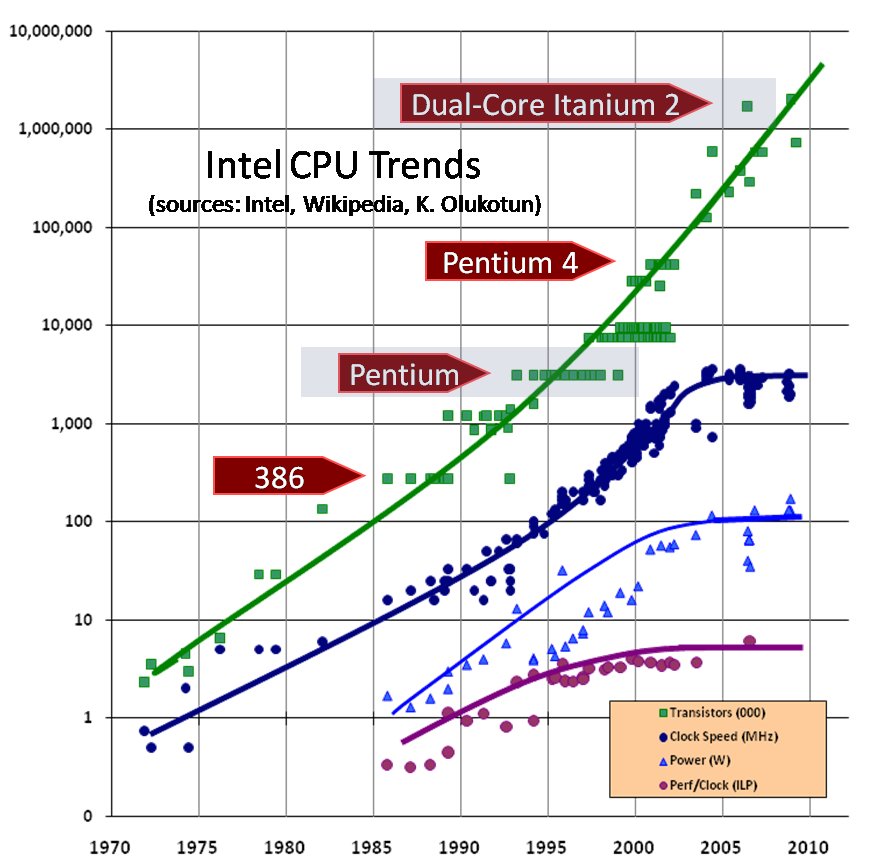
\includegraphics[width=12cm,height=8cm]{1-Introduction/Figures/Moore.png}
  \end{tabular}
  \end{center}
   \caption{\label{fig:CPU_Trend} روند افزایش سرعت پردازنده‌ها در سال‌های اخیر\cite{Sutter05thefree}}
\end{figure}
%\section{صورت مسئله} 
%موضوع این پژوهش بررسی روش طراحی منطق دامنه با استفاده از تبادل ناهمگام پیغام می‌باشد. در این روش اشیاء
%در طراحی به روش تبادل ناهمگام پیغام، علاوه بر نکات مربوط به طراحی شیءگرای ترتیبی، 
 
%\section{روش پژوهش}
%ارزیابی عملی با مطالعه‌ی موردی

\section{خلاصه‌ی دستاوردهای پژوهش}
برخی از دستاوردهای این پژوهش را می‌توان به این ترتیب برشمرد:
\begin{itemize}
\item  یک سیستم نمونه انتخاب شده و طراحی منطق دامنه‌ی آن به روش تبادل ناهمگام پیغام به طور کامل انجام شده است. ارائه‌ی روش طراحی به صورت مرحله‌ای و افزایشی باعث شده است تا بتوان از آن به صورت دستورالعملی برای طراحی همروند استفاده کرد. 
\item خروجی اصلی این پژوهش، روش‌ها و الگوهایی است که در این نوع طراحی کاربرد دارد. در هر الگوی استخراج شده، روش پیاده‌سازی در مدل اکتور و کاربردهای الگو از نظر منطق دامنه بررسی شده است. 
\item تجربیاتی که در طراحی‌های صورت گرفته کسب شده به صورت قابل استفاده‌ای ارائه شده است و مطالعه‌ی این تجربیات، خواننده را با نکات ظریف و  حساسی آشنا می‌کند که انجام طراحی به روش تبادل ناهمگام پیغام را بسیار ساده‌تر می‌کند.
\item در ارزیابی روش طراحی ناهمگام، خصوصیات کیفی این روش از جمله تغییرپذیری و کارایی آن با روش طراحی شیءگرای ترتیبی مقایسه شده و نشان داده شده است که علاوه بر اینکه از نظر تغییرپذیری دو روش قابل مقایسه هستند، طراحی به روش تبادل ناهمگام پیغام در مواردی باعث افزایش چشم‌گیر کارایی سیستم می‌گردد.
\end{itemize}
\section{ساختار پایان‌نامه}
برای بررسی این موارد، ساختار این متن در ۷ فصل تنظیم گردیده است:
\begin{strict_itemize}
\item  فصل ۲ به ارائه‌ی برخی پیش‌نیازهای طراحی به روش تبادل ناهمگام پیغام می‌پردازد. مدل اکتور و کتابخانه‌ی اکتور اسکالا در این فصل معرفی شده‌اند.
\item در فصل ۳ پژوهش‌های مرتبط معرفی شده‌اند. الگوهای طراحی با اکتورها و نیز کاربردهای صنعتی رویکرد تبادل ناهمگام پیغام در این فصل بررسی شده‌اند. علاوه بر آن روش‌های طراحی منطق دامنه در برنامه‌نویسی شیءگرا به طور مختصر معرفی شده‌اند.
\item در فصل ۴ یک سیستم نمونه تعریف شده و با استفاده از رویکرد تبادل ناهمگام پیغام طراحی شده است.
\item در فصل ۵ روش طراحی منطق دامنه با استفاده از تبادل ناهمگام مورد بررسی قرار گرفته‌ است و الگوهای طراحی استخراج شده‌ از طراحی سیستم نمونه، ارائه شده‌اند.
\item  در فصل ۶ معیارهای کیفی سیستم طراحی شده با رویکرد تبادل ناهمگام بررسی شده و با همین‌ ویژگی‌ها در رویکرد طراحی شیءگرای ترتیبی مقایسه شده است.
\item نهایتا فصل ۷ به جمع‌بندی پژوهش، ارائه‌ی دستاوردها و ذکر تعدادی از جهت‌گیری‌های مرتبط برای پژوهش‌های آینده می‌پردازد.
\end{strict_itemize}

\chapter{پیش‌زمینه تحقیق}
\label{chapter:Preliminaries}
\thispagestyle{plain}
در این فصل به طور اجمالی مروری بر پیش‌زمینه‌ی پژوهش انجام شده است. در هر بخش سعی شده است که با حفظ اختصار، تنها جنبه‌های  کاربردی مرتبط با پژوهش مطرح گردد.
\section{مدل اکتور}
\label{section:actorModel}

در زمینه‌ی برنامه‌نویسی همروند پژوهش‌های مختلفی صورت گرفته و مدل‌هایی ارائه شده است\cite{Briot98concurrencyand}. در این میان مدل \gls{اکتور}\LTRfootnote{Actor Model} با توجه به استفاده از ارتباط ناهمگام و قابلیت توزیع بالا توجه زیادی را به خود جذب کرده است. با توجه به ارتباط تنگاتنگ این مدل با پژوهش حاضر، در این بخش به معرفی اجمالی این مدل می‌پردازیم.
لفظ اکتور برای اولین بار در حدود ۳ دهه پیش توسط هیوئیت  \cite{Hewitt1972} به کار گرفته شد. اکتور در کاربرد هیوئیت به معنی موجودیت‌های فعالی بود که در یک پایگاه دانش به جستجو پرداخته و در نتیجه کنش‌هایی را ایجاد می‌نمودند. در دهه‌های بعدی گروه هیوئیت با تکیه بر اکتورها به عنوان عامل‌های محاسباتی\LTRfootnote{agents of computation} مدل اکتور را به عنوان یک مدل محاسباتی همروند گسترش داد. خلاصه‌ای از تاریخچه‌ی مدل بازیگر در \cite{AghaMST97} موجود است. امروزه برداشت عمومی از مدل اکتور مربوط به  آقا\cite{Agha_86} می‌باشد. در ادامه‌ی این بخش مشخصات مدل اکتور ارائه شده است.
 
مدل اکتور که توسط هیوئیت و آقا \cite{Hewitt1972,Agha1987,Agha1990} ایجاد شده‌است، یک نمایش سطح بالا از سیستم‌های توزیع‌شده فراهم می‌کند. 
\gls{اکتور}هااشیای \gls{لفافه‌بندی‌شده}‌ای هستند که به صورت \gls{همروند} فعالیت می‌کنند و دارای \gls{رفتار}\LTRfootnote{Behavior} قابل تغییر هستند. 
اکتورها \gls{حالت  مشترک}\LTRfootnote{Shared State} ندارند و تنها راه ارتباط بین آنها تبادل ناهمگام پیغام است. 
 در مدل اکتور فرضی در مورد مسیر پیغام و میزان تاخیر در رسیدن پیغام وجود ندارد، در نتیجه ترتیب رسیدن پیغام‌ها \gls{غیرقطعی} است.
 در یک دیدگاه می‌توان اکتور را یک \gls{شی‌ء} در نظر گرفت که به یک ریسمان\gls{ریسمان}\LTRfootnote{Thread} کنترل، یک صندوق پست و یک نام غیر قابل تغییر و به صورت سرارسی یکتا \LTRfootnote{Globally Unique} مجهز شده است. برای ارسال پیغام به یک اکتور، از نام آن استفاده می‌شود. در این مدل، نام  یک اکتور را می‌توان در قالب پیغام  ارسال کرد. پاسخگویی به هر پیام شامل برداشتن آن پیام از صندوق پستی و اجرای عملیات متناسب با آن است.
این اجرای عملیات به صورت \gls{تجزیه‌ناپذیر}\LTRfootnote{Atomic} و بی‌وقفه خواهد بود\cite{Agha_86}.

\begin{figure*}
    \begin{center}
	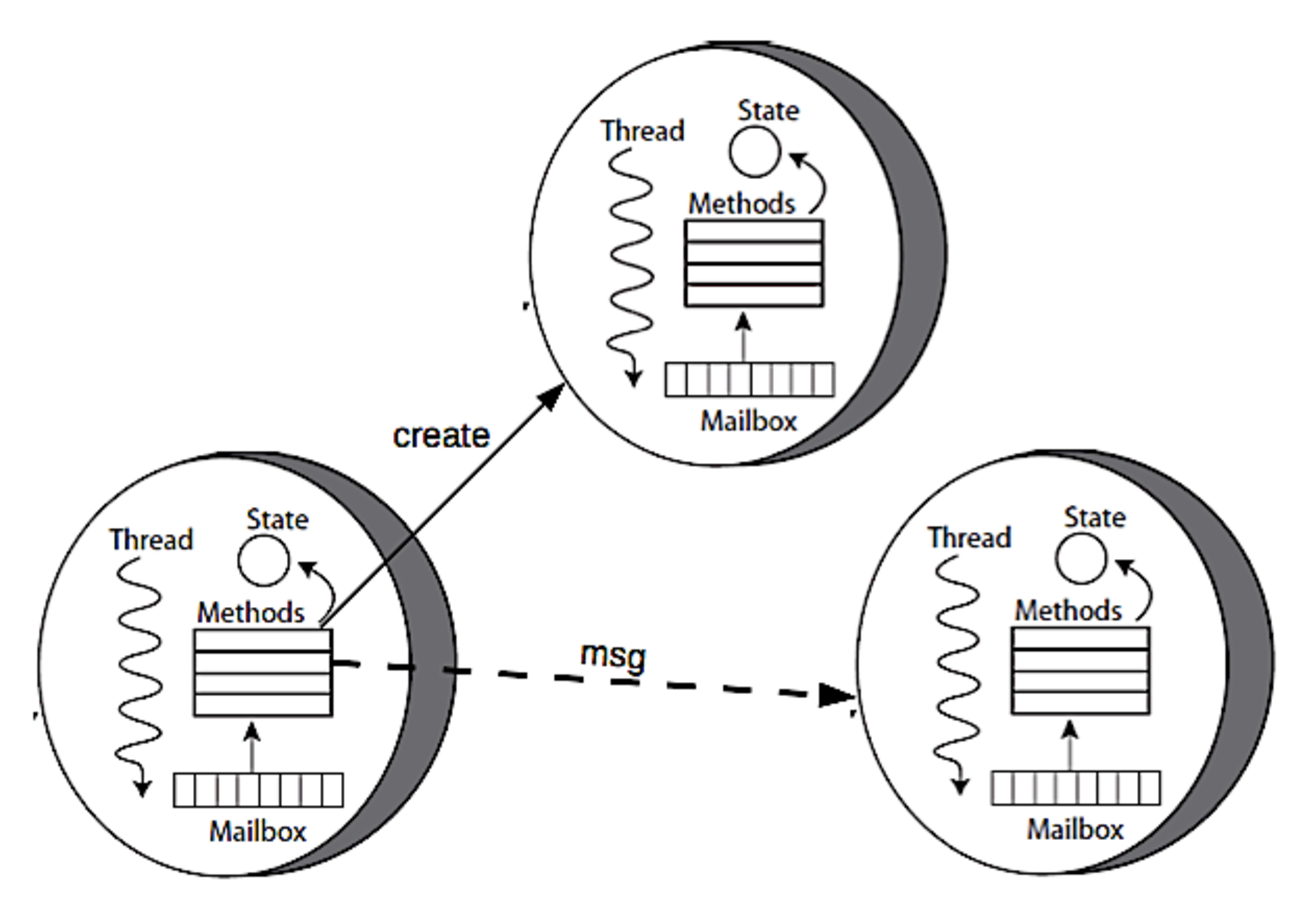
\includegraphics[width=12cm]{2-Preliminaries/Figures/Actor_Structure.pdf}
    \end{center}
    \caption{\label{fig:actorStructure} اکتور‌ها موجودیت‌های همروندی هستند که به صورت ناهمگام تبادل پیغام انجام ‌می‌دهند. }
\end{figure*}


همان گونه که گفته‌شد، مدل اکتور سیستم را در سطح بالایی از انتزاع مدل می‌کند.
این ویژگی دامنهٔ سیستم‌های قابل مدلسازی توسط مدل اکتور را بسیار وسیع نموده‌است.
انواع سیستم‌های سخت‌افزاری و نرم‌افزاری طراحی‌شده برای زیرساخت‌های خاص یا عام، و همچنین الگوریتم‌ها و پروتکل‌های توزیع‌شدهٔ مورد استفاده در شبکه‌های ارتباطی از جملهٔ موارد مناسب برای بهره‌گیری از مدل اکتور هستند. علاوه بر این، خصوصیت تبادل ناهمگام پیغام، باعث می‌شود مدل اکتور برای مدل کردن سیستم‌های توزیع شده و متحرک بسیار ایده‌آل باشد\cite{KarmaniAgha_Actors_11}. شکل \ref{fig:actorStructure} شمای کلی از مدل اکتور و نحوه‌ی تعامل اکتور‌ها را نشان می‌دهد.
 
 یک اکتور در نتیجه‌ی دریافت پیغام احتمالا محاسباتی انجام می‌دهد و در نتیجه‌ی آن یک از ۳ عمل زیر را انجام می‌دهد:
\begin{itemize}
\item ارسال پیغام به سایر اکتور‌ها
\item ایجاد اکتور جدید
\item تغییر حالت محلی
\end{itemize} 

\subsection{\gls{معناشناسی}}\LTRfootnote{Semantics}
از نظر معناشناسی مشخصه‌های کلیدی مدل محض اکتور عبارتند از: لفافه‌بندی و
  \gls{تجزیه‌ناپذیر}‌ی\LTRfootnote{Encapsulation and Atomicity}، \gls{انصاف}\LTRfootnote{Fairness}، 
  استقلال از مکان\LTRfootnote{Location Transparency}، توزیع\LTRfootnote{Distribution} و تحرک\LTRfootnote{Mobility}
 \cite{KarmaniAgha_Actors_11}. 
  باید توجه داشت که این مشخصه‌ها در مدل محض  وجود دارند و این الزاما به این معنی نیست که تمام زبان‌های مبتنی بر مدل اکتور از این مشخصه‌ها پشتیبانی می‌کنند. ممکن است تعدادی از این مشخصه‌ها در  زبان‌های مبتنی بر اکتور  با در نظر گرفتن اهدفی مانند کارایی و سهولت پیاده‌سازی نشده‌اند. در این موارد باید با به کار بردن ابزار‌های بررسی ایستا، مترجم‌ها و یا با تکیه بر عملکرد درست برنامه‌نویس از صحت عملکرد برنامه‌ اطمینان حاصل کرد \cite{ActorsJVM2009}. 
\begin{itemize}
\item \textbf{لفافه‌بندی و \gls{تجزیه‌ناپذیر}ی:}\LTRfootnote{Encapsulation and Atomicity}  
نتیجه‌ی مستقیم مشخصه‌ی لفافه‌بندی در اکتور‌ها این است که درهیچ دو اکتوری، به اشتراک گذاری حالت وجود ندارد. این مشخصه، \gls{تجزیه}ی \gls{شیءگونه}ی برنامه را تسهیل می‌کند. در زبان‌های برنامه‌نویسی \gls{شیء-بنیاد} مشخصه منجر به ایجاد تغییر تجزیه‌ناپذیر شده است. به این صورت که وقتی یک شیء، شیء دیگری را فراخوانی می‌کند، شیء مقصد تا پایان محاسبات مربوط به این فراخوانی، به فراخوانی‌های دیگر پاسخ نمی‌دهد.  این مشخصه به ما اجازه می‌دهد تا بتوانیم در باره‌ی رفتار یک شیء در قبال دریافت یک پیغام (فراخوانی) با توجه به حالت شیء در زمان دریافت آن \gls{استدلال} کنیم.

در محاسبات همروند، وقتی یک اکتور مشغول انجام محاسبات مربوط به یک پیغام است، امکان دریافت پیغام جدید توسط آن وجود دارد اما مشخصه‌ی تجزیه‌ناپذیری تضمین می‌کند که پیغام جدید امکان قطع محاسبات جاری اکتور و تغییر حالت محلی آن را ندارد. این مشخصه الزام می‌کند که اکتور گیرنده، در هر لحظه فقط یک پیغام در حال پردازش داشته باشد و محاسبات مربوط به  پیغام جاری را در یک قدم بزرگ\LTRfootnote{Macro-Step} به صورت تجزیه ناپذیر طی کند. \cite{AghaMST97}
مشخصه‌های معناشناسی لفافه‌بندی و تجزیه ناپذیری به طور  چشم‌گیری از عدم قطعیت مدل اکتور می‌کاهند و با کوچکتر کردن فضای حالت برنامه‌های نوشته شده در مدل اکتور، این برنامه‌ها را برای استفاده در ابزارهای آزمون درستی و  verification(?) قابل استفاده می‌کند\cite{LauterburgKMA10}.
این دو مشخصه مجموعا باعث می‌شوند تا بتوانیم بر اساس پیغام انتخاب شده برای اجرا و وضعیت محلی اکتور در هنگام شروع به اجرا ، رفتار یک اکتور قابل پیش‌بینی باشد.

\item \textbf{ \gls{انصاف}:}
انصاف در مدل اکتور به این مفهوم است که پیغام فرستاده شده نهایتا به اکتور مقصد خواهد رسید، مگر آنکه اکتور مقصد به طور دائمی غیر فعال شده باشد. لازم به ذکر است که این تعریف از  انصاف در رسیدن پیغام به اکتور مقصد، متضمن انصاف در \gls{زمان‌بندی} اکتور‌ها است. به این مفهوم که در صورتی که یک اکتور در اثر  زمان‌بندی غیر منصفانه، موفق به اخذ نوبت اجرا نشود، پیغام‌های فرستاده شده به مقصد آن اکتور هرگز به مقصد نخواهند رسید. انصاف علاوه بر تضمین رسیدن پیغام‌ها، امکان استدلال مناسب درباره‌ی نحوه‌ی تداوم اجرای  برنامه‌\LTRfootnote{Liveness Property} را فراهم می‌کند. میزان طبیعتا میزان موفقیت در تضمین این مشخصه در محیط‌های مبتنی بر اکتور وابسته به منابع موجود در سیستم در حال اجرا است \cite{ActorsJVM2009}.
\item \textbf{ استقلال از مکان، توزیع و تحرک:}
\label{mobility}
در مدل اکتور، ارسال پیغام به یک اکتور تنها از طریق دسترسی به نام آن اکتور ممکن می‌شود. مکان واقعی اکتور تأثیری روی نام آن ندارد. هر اکتور دارای فضای آدرس مربوط به خود است که می‌تواند کاملا متفاوت با دیگر اکتور‌ها باشد. اکتورهایی که به یکدیگر پیغام می‌فرستند می‌توانند روی یک هسته از یک پردازنده‌ی مشترک اجرا شوند یا اینکه در ماشین دیگری که از طریق شبکه به آنها مرتبط می‌شوند در حال اجرا باشند. مشخصه‌ی  استقلال از مکان در مدل اکتور به برنامه‌نویس این امکان را می‌دهد که فارغ از نگرانی درباره‌ی محل اجرای  اکتور ها به برنامه‌نویسی بپردازد.
 عدم اطلاع از مکان اجرای اکتوران  منجر به قابلیت حرکت در آنها می‌شود. تحرک به صورت قابلیت انتقال پردازش به نودهای دیگر تعریف می‌شود.در سطح سیستم، تحرک از جهت توزین بار \LTRfootnote{Load-Balancing}، قابلیت تحمل خطا\LTRfootnote{Fault Tolerance} و نیز پیکربندی مجدد\LTRfootnote{Reconfiguration} حائز 
 اهمیت است.
 پژوهش‌های پیشین نشان می‌دهد که قابلیت تحرک در رسیدن به کارایی \gls{مقیاس‌پذیر} به ویژه در کاربردهای  \gls{بی‌قاعده}\LTRfootnote{Irregular} روی ساختار داده‌های \gls{پراکنده} مفید است\cite{KimA95}. در کاربردهای دیگر، توزیع بهینه به شرایط زمان اجرا و میزان بار وابسته است. به عنوان مثال، در کاربردهای وب، تحرک با توجه به شرایط شبکه و امکانات کلاینت مورد استفاده قرار می‌گیرد\cite{ContextAwareWeb}.  
از سوی دیگر، قابلیت تحرک می‌تواند در کاهش انرژی مصرفی در اثر اجرای کاربردهای موازی مفید باشد. در این کاربردها، محاسبات موازی به صورت پویا بین تعداد هسته‌های بهینه (تعداد هسته‌هایی که منجر به کمترین مصرف می‌شوند) توزین می‌شوند. قسمت‌های مختلف یک کاربرد می‌تواند شامل الگوریتم‌های موازی مختلفی باشد و میزان مصرف انرژی یک الگوریتم به تعداد هسته‌های مشغول اجرای الگوریتم و نیز بسامد اجرای آن هسته‌ها بستگی دارد\cite{KorthikantiA10}. در نتیجه، ویژگی تحرک پذیری اکتور‌ها، ویژگی مهمی برای برنامه نویسی در معماری‌های چند-هسته‌ای به شمار می‌آید.

\end{itemize} 


\subsection{پیاده‌سازی‌ها}
\label{subsection:actorImpls}
برای مدل اکتور زبان‌ها و چارچوب‌های زیادی توسعه داده شده است. ABCL، POOL، ConcurrentSmalltalk، ACT++ و CEiffel تعدادی از پیاده‌سازی‌های اولیه از این مدل می‌باشند. مرجع \cite{Briot98concurrencyand} به بررسی این زبان‌ها پرداخته است. شاید بتوان زبان  \gls{ارلانگ}\LTRfootnote{Erlang}\cite{erlang} را معروفترین پیاده‌سازی مدل اکتور دانست. این زبان در حدود ۲۲ سال قبل برای برنامه‌نویسی سوئیچ‌های مخابراتی شرکت اریکسون\LTRfootnote{Ericsson} توسعه داده شد. علاوه بر ارلانگ زبان‌ها و چارچوب‌های مبتنی بر مدل اکتور دیگری نیز در سال‌های اخیر مورد استفاده گرفته‌اند که کتابخانه‌ی اکتور اسکالا
\LTRfootnote{Scala Actor Library} \cite{ScalaActors}،  Ptolemy \cite{Ptolemy}، SALSA \cite{salsa}، CHARM++ \cite{CHARMplus}، ActorFoundry \cite{ActorFoundry}، Asynchronous Agents Library \cite{AsyncAgentsLib}  از جمله‌ی آنها هستند.
  از کاربردهای متن-باز که بر مبنای مدل اکتور توسعه داده شده‌اند می‌توان به سیستم تبادل پیغام توئیتر\LTRfootnote{Twitter} و چارچوب تحت وب لیفت\LTRfootnote{Lift} و از میان کاربرد‌های تجاری می‌توان به سیستم گپ\LTRfootnote{Chat} فیسبوک و موتور بازی وندتا\LTRfootnote{Vendetta game engine} اشاره کرد.
در این پژوهش برای پیاده‌سازی نسخه‌ی مبتنی بر تبادل ناهمگام پیغام از کتابخانه‌ی اکتور اسکالا استفاده شده است (چرا؟) که در بخش ؟ معرفی شده است.


\section{معرفی زبان اسکالا و کتابخانه‌ی اکتور اسکالا}
\label{section:Scala}
همان طور که در بخش \ref{subsection:actorImpls} اشاره شد، پیاده‌سازی‌های مختلفی از مدل اکتور در زبان‌ها و چارچوب‌های برنامه‌نویسی ارائه شده است. مقاله‌ی \cite{ActorsJVM2009} به بررسی و مقایسه‌ی این پیاده‌سازی‌ها پرداخته است. در این پژوهش زبان اسکالا و کتابخانه‌ی اکتور آن برای پیاده‌سازی مطالعه‌ی موردی انتخاب شده است. گستردگی ابزار و همچنین فعال بودن جامعه\LTRfootnote{Community}‌ی برنامه‌نویسی این زبان اصلی‌ترین انگیزه‌های انتخاب این زبان برای پیاده‌سازی بوده‌اند. ضمنا با توجه به انتخاب زبان جاوا برای پیاده‌سازی نسخه‌ی متداول مورد مطالعه و ارتباط تنگاتنگ زبانهای اسکالا و جاوا، انتخاب زبان اسکالا منجر به سهولت ارزیابی مقایسه‌ای مطالعه‌ی موردی شده است. در این بخش به معرفی اجمالی زبان اسکالا و کتابخانه‌ی اکتور آن پرداخته شده است. هدف از این معرفی، سهولت درک روش طراحی پیشنهادی در فصل ۳ می باشد و به همین دلیل از توضیح جزئیات و امکانات اضافی این زبان خودداری شده است. کتاب \cite{programmingInScala} به عنوان منبع این بخش استفاده شده است.
\subsection{زبان اسکالا}
اسکالا مخفف عبارت \emph{''زبان مقیاس‌پذیر``}\LTRfootnote{Scalable Language} است و اشاره به این نکته دارد که اسکالا برای رشد بر اساس نیاز کاربر طراحی شده است. اسکالا را می‌توان برای گستره‌ی وسیعی از کاربردها از نوشتن اسکریپت‌های کوچک گرفته تا پیاده‌سازی سیستم‌های بزرگ به کار برد. برنامه‌های اسکالا بر روی محیط اجرایی جاوا\LTRfootnote{JRE}  قابل اجرا هستند و در برنامه‌های اسکالا  می‌توان از کتابخانه‌های استاندارد جاوا استفاده کرد.
زبان اسکالا ترکیبی از ویژگی‌های زبان‌های \gls{تابعی} و شیءگرا را در خود دارد. در زبان‌های تابعی، توابع مانند انواع داده‌ها قابل ارجاع هستند. اسکالا مانند جاوا دارای \gls{بررسی گونه‌ها}ی، \gls{ایستا} است.
\codelisting[language=scala]{2-Preliminaries/src/Sample.scala}{قطعه کد نمونه برای زبان اسکالا}{figure:scalaSample}

در ادامه مشخصات نحوی زبان اسکالا در قالب یک مثال توضیح داده می‌شود. در شکل \ref{figure:scalaSample} قطعه کد اسکالا مربوط به کلاس Course نمایش داده شده است. برای آشنایی با نحو زبان اسکالا به بررسی این کد می‌پردازیم:\\
در خطوط ۱و ۲ کلاس Course و متغیرهای ،id ،name units و prerequisites به عنوان فیلد‌های آن تعریف شده‌اند. در خط ۴ تابع equals از این کلاس override شده است. در اسکالا همانند جاوا هر کلاس به طور پیش‌فرض دارای یک تابع‌ equals است که در صورت لزوم می‌توان آن را override کرد. همان‌طور که در کد مشخص است، تعریف تابع در اسکالا با کلمه‌ی کلیدی  \textbf{def} انجام می‌گیرد. در خطوط ۴ تا ۸ شرط لازم برای یکسان بودن یک شیء از نوع Course با شیء حاضر پیاده‌سازی شده است. نوع و مقدار یک متغیر را می‌توان با استفاده از دستور \lr{match .. case .. } با انواع و مقادیر دلخواه مقایسه کرد. نتیجه‌ی دستورات خطوط ۶ و ۷ این است که اگر متغیر other از نوع Course باشد و مقدار فیلد id آن با مقدار فیلد id از شیء حاضر یکسان باشد تابع مقدار true را برمی‌گرداند. خط ۸ به این معنا است که اگر هر حالت دیگری به جز حالت قبل بود مقدار false برگردانده ‌می‌شود. در خط ۱۲ ‌نمونه‌ای از حلقه‌ی for نمایش داده شده است. در اسکالا حلقه‌ها به صورت‌های متنوعی می‌توانند بیان شوند که در این مثال یک حالت از آنها نمایش داده شده است.  در خط ۱۲ متغیر pre برای گرفتن مقدار موقت حلقه تعریف شده است. نکته‌ی جالب توجه این است که در این خط، نوع متغیر تعریف نشده است. در بخش قبل ذکر شد که اسکالا دارای خاصیت بررسی گونه‌های ایستا \LTRfootnote{static type checking} است. ظاهرا این دو امر در تناقض با یکدیگر هستند اما باید توجه داشت که در زبان اسکالا نوعی از استنتاجِ گونه\LTRfootnote{type inference} در زمان ترجمه اتفاق می‌افتد. در این مورد با توجه به اینکه متغیر pre از لیست prerequisites مقداردهی می‌شود، گونه‌ی آن در زمان ترجمه قابل استنتاج است. خط ۱۶ تابع دیگری را نشان می‌دهد که در آن تابع toString، override شده است. نکته‌ی قابل توجه در مورد این قسمت از کد عدم استفاده از علامت \{ \} برای تعیین حوزه‌ی تابع است. در زبان اسکالا به دلیل وجود ویژگی‌های زبان‌های تابعی، می‌توانیم با توابع مانند متغیر‌ها و داده‌ها رفتار کنیم که این بخش از کد مثالی از این ویژگی است. همانطور که در این مثال مشخص است، در زبان اسکالا استفاده از نقطه‌ویرگول (;) در اکثر موارد اختیاری است.

\subsection{کتابخانه‌ی اکتور اسکالا}
\label{section:scalaActorLib}
همانطور که در بخش \ref{subsection:actorImpls} اشاره شد، یکی از پیاده‌سازی‌های مدل اکتور، کتابخانه‌ی اکتور اسکالا است. در این بخش به معرفی اجمالی کتابخانه‌ی اکتور اسکالا و طرز استفاده از آن برای برنامه‌نویسی همروند می‌پردازیم.
\subsubsection{ایجاد اکتور}
اکتور‌ها در اسکالا از کلاس scala.actors.Actor مشتق می‌شوند.  شکل \ref{figure:sillyActor} کد مربوط به  یک اکتور ساده را نشان می‌دهد. این اکتور کاری به صندوق پیغام‌ها ندارد و صرفا پنج بار پیغام \lr{I'm acting!} را چاپ می‌کند و سپس اجرای آن خاتمه می‌یابد.

\codelisting[language=scala]{2-Preliminaries/src/SillyActor.scala}{کد یک اکتور ساده در زبان اسکالا}{figure:sillyActor}

  اکتور‌ها در اسکالا با دستور start() شروع به فعالیت می‌کنند. با شروع به فعالیت یک اکتور، تابع act() آن فراخوانی می‌شود و تا زمانی که اجرای این تابع به اتمام نرسد، اکتور به طور همروند در حال اجرا باقی می‌ماند. در صورتی که بخواهیم اکتور به طور دائمی در حال اجرا بماند دو راه وجود دارد. راه اول این است که تابع act() را در پایان کار  خود مجدداً فراخوانی کنیم. و راه دیگر استفاده از عبارت \textbf{loop} در اسکالا است. دستورات درون حلقه‌ی loop به صورت بی‌پایان اجرا می‌شوند. شکل \ref{fig:endlessActor} کدهای مربوط به این ۲ روش را نمایش می‌دهد.

\begin{figure*}
    \begin{center}
    \begin{tabular}{ c  c }
      	%\hline
	 & \\

	\begin{latin}
\linespread{1.1}
\lstinputlisting[language=scala]{2-Preliminaries/src/SillyActor2.scala}
\end{latin} & 
 \begin{latin}
	\linespread{1.1}
	\lstinputlisting[language=scala]{2-Preliminaries/src/SillyActor3.scala}
\end{latin}
 	\\
         (الف) & (ب) \\
%	\hline
    \end{tabular}
    \end{center}
    \caption{\label{fig:endlessActor} تداوم اجرای اکتور با استفاده از الف)فراخوانی بازگشتی و ب)حلقه‌ی loop}
\end{figure*}


\subsubsection{تبادل پیغام}
عملگر \textbf{!} برای فرستادن پیغام ناهمگام استفاده می‌شود. دستور \lr{dest ! message} پیغام message را برای اکتور dest ارسال می‌کند بدون آنکه برای دریافت جواب منتظر بماند. با اینکه در مدل اکتور دستوری برای تبادل همگام پیغام وجود ندارد، در اکثر پیاده‌سازی‌ها این امکان به مدل اضافه شده است\cite{ActorsJVM2009}. در کتابخانه‌ی اکتور اسکالا، عملگر \lr{!?} به این منظور به کار گرفته می‌شود. در صورت استفاده از این دستور، فرستنده‌ی پیغام تا گرفتن جواب متوقف می‌ماند. برای برداشتن پیغام از صندوق پیغام‌ها، از دو دستور receive و react استفاده می‌شود (تفاوت این دو دستور در بخش \ref{ref:receive_react} توضیح داده شده است). شکل \ref{fig:pingPongActor} مثالی از نحوه‌ی تبادل پیغام بین اکتوران را نمایش می‌دهد. در این برنامه دو اکتور PingActor و PongActor به تبادل پیغام می‌پردازند. در ابتدا اکتور PingActor که متغیر آن با مقدار ۱۰۰ مقداردهی شده است یک پیغام Ping برای اکتور PongActor می‌فرستد و در ادامه در یک حلقه‌ی loop منتظر پاسخ Pong می‌ماند. اکتور PongActor با گرفتن هر پیغام Ping پاسخ Pong را برای فرستنده ارسال می‌کند. کلمه‌ی کلیدی \textbf{sender} در کلاس Actor اشاره‌گری به فرستنده‌ی پیغام در حال پردازش ‌می‌باشد (خط ۶ از کد قسمت (ب) شکل \ref{fig:pingPongActor}). اکتور PingActor با دریافت پاسخ‌ Pong مقدار متغیر pingsLeft را چک می‌کند و در صورت مثبت بودن آن پیغام Ping بعدی را ارسال می‌کند و در غیر این صورت پیغام Stop را ارسال ‌می‌کند. نهایتا با صفر شدن متغیر pingsLeft، اکتور PingActor پیغام Stop را برای PongActor می‌فرستد. دستور exit که در پایان کار هر دو اکتور استفاده شده است باعث می‌شود ریسمان اجرایی اکتور رها شود و پس از اجرای این دستور اکتور قادر به دریافت پیغام نخواهد بود.

\begin{figure*}
    \begin{center}
    \begin{tabular}{ c }
 \begin{latin}
	\linespread{1.1}
	\lstinputlisting[language=scala]{2-Preliminaries/src/Ping.scala}
\end{latin}
\\ 
\scriptsize{(الف) اکتور Ping که فرستنده‌ی اولیه‌ی پیغام است}
&
\hline
\\
\begin{latin}
\linespread{1.1}
\lstinputlisting[language=scala]{2-Preliminaries/src/Pong.scala}
\end{latin}  
\\
\scriptsize{(ب) اکتور Pong که به پیغام ping پاسخ می‌دهد.}
          &
\hline
\begin{latin}
\linespread{1.1}
\lstinputlisting[language=scala]{2-Preliminaries/src/PingPong.scala}
\end{latin} 
\\
\scriptsize{(ج) کد اجرای برنامه‌ی PingPong}
         &
\hline

\end{tabular}
\end{center}
\caption{\label{fig:pingPongActor} مثالی از نحوه‌ی تبادل پیغام بین اکتور‌ها}
\end{figure*}

\subsubsection{ زیرساخت اجرای همروند در کتابخانه‌ی اکتور اسکالا}
\label{ref:receive_react}
پردازش‌های همروند مانند اکتور‌ها با دو نوع استراتژی پیاده‌سازی می‌شوند:
\begin{itemize}
\item \textbf{پیاده‌سازی \gls{ریسمان-بنیان}:}
در این نوع پیاده‌سازی رفتار پردازش همروند به وسیله‌ی یک ریسمان کنترل می‌شود. حالت اجرا\LTRfootnote{execution state} به وسیله‌ی  \gls{پشته}‌ی ریسمان\cite{concurrent_prog_java}

\item \textbf{پیاده‌سازی \gls{رویداد-بنیان}:}
در این مدل رفتار به کمک یک سری \gls{مجری رویداد}\LTRfootnote{event handler} پیاده‌سازی می‌شوند. این مجری‌ها از یک حلقه‌ی رویداد فراخوانی می‌شوند. حالت اجرای پردازش‌های همروند در این روش به کمک رکورد‌ها یا اشیاء مشخصی که به همین منظور طراحی شده‌اند نگهداری می‌شود \cite{SEDA}.
\end{itemize}
مدل ریسمان-بنیان معمولا پیاده‌سازی راحتتری دارد ولی به دلیل مصرف حافظه‌ی بالا و پرهزینه بودن \gls{تعویض متن}\LTRfootnote{context switch} می‌تواند منجر به کارایی کمتری شود\cite{WhyThreadsAreABadIdea}. از طرف دیگر مدل رویداد-بنیان معمولا کاراتر است ولی در طراحی‌های بزرگ پیاده‌سازی آن مشکل‌تر است\cite{whyevents}.
استفاده از مدل رویداد-بنیان منجر به ایجاد نوعی از \gls{وارونگی کنترل}\LTRfootnote{Inversion of Control} می‌شود: یک برنامه به جای فراخوانی عملیات \gls{مسدود کننده} \LTRfootnote{blocking operation}، صرفا تمایل خود به ادامه‌ی کار در صورت رخ دادن رویدادهای مشخص (مانند فشردن یک دکمه) را به محیط اجرا اعلام می‌کند. این اعلام تمایل با ثبت یک مجری رویداد در محیط انجام می‌شود. برنامه هیچ وقت این مجری‌های رویداد را فراخوانی نمی‌کند بلکه محیط اجرایی با وقوع هر رخداد، مجری‌های ثبت شده برای آن رویداد را فراخوانی می‌کند. به این ترتیب کنترل اجرای منطق برنامه نسبت به حالت بدون رویداد \textbf{وارونه} می‌شود. به دلیل پدیده‌ی وارونگی کنترل، تبدیل یک مدل ریسمان-بنیان به مدل رویداد-بنیان معادل معمولا نیاز به دوباره‌نویسی برنامه دارد\cite{responders2006}.
\\
در پیاده‌سازی زیرساخت همروندی در کتابخانه‌ی اکتور اسکالا هر دو رویکرد معرفی شده پیاده‌سازی شده‌اند و قابل دسترسی هستند. اصلی‌ترین عمیات مسدود کننده در مدل اکتور انتظار برای دریافت پیغام است. کنترل اجرا در صورتی مسدود می‌شود که پیغامی که اکتور منتظر دریافت آن است در صندوق پیغام موجود نباشد. در اکتور‌های اسکالا، عمل برداشتن پیغام با دو دستور انجام می‌شود:
\begin{itemize}
\item دستور receive:
با استفاده از این دستور، در صورتی که در صندوق پیغام اکتور، پیغامی که با یکی از الگوهای معرفی شده در بدنه‌ی receive موجود باشد کد مربوط به الگوی‌ مربوطه اجرا می‌شود. در غیر این صورت ریسمان اجرای این اکتور مسدود می‌شود. در این حالت پشته‌ی فراخوانی تابع act() در اکتور به صورت خودکار توسط محیط اجرایی ذخیره می‌شود و در صورت ورود پیغام متناسب اجرا به صورت ترتیبی از سر گرفته می‌شود. بنابراین در پیاده‌سازی این دستور از رویکرد ریسمان-بنیان استفاده شده است.
\item دستور react:
با استفاده از این دستور، در صورتی که هیچ پیغام متناسبی در صندوق پیغام وجود نداشته باشد، به جای مسدود کردن ریسمان اجرای اکتور، از رویکرد رویداد-بنیان استفاده می‌شود. این کار از طریق نوع خاصی از تابع در زبان اسکالا انجام می‌شود که هیچ‌گاه به طور معمولی اجرای آن خاتمه نمی‌یابد. بلکه پس از ثبت مجری رویداد مناسب در محیط اجرا، با استفاده از ایجاد یک \gls{استثناء}\LTRfootnote{exception} اجرای تابع react و توابع شامل آن در اکتور خاتمه می‌یابد. در این نوع توقف اجرا با توجه به اینکه ریسمان اجرا مسدود نمی‌شود، پشته‌ی فراخوانی تابع نیز ذخیره نمی‌شود و با برگشت به اجرای این تابع، محیط هیچ تاریخچه‌ای از اجرای قبلی آن ندارد. در نتیجه در هر بار بازگشت مانند اولین اجرا رفتار می‌کند. نتیجه‌ی مهم این خصوصیت این است که در صورت استفاده از react در یک اکتور، هیچ کدی که بعد از این تابع نوشته شده باشد اجرا نخواهد شد. به همین دلیل برنامه‌نویس باید دقت کند که تابع react از نظر ترتیب اجرا همیشه آخرین کد بدنه‌ی یک اکتور باشد.
نتیجه‌ی استفاده از رویکرد رویداد-بنیان در اکتور‌های اسکالا افزایش چشمگیر کارایی در صورت استفاده از تعداد بسیار زیاد اکتور در سیستم است. 
\end{itemize}
به برنامه نویسان توصیه شده است که به جز در موارد خاص که نیاز به مسدود کردن ریسمان اجرای اکتور وجود دارد، در بقیه‌ی موارد از رویکرد رویداد-بنیان استفاده کنند. توضیحات تکمیلی در مورد نحوه‌ی پیاده‌سازی هر دو رویکرد در کتابخانه‌ی اکتور اسکالا و آنالیز کارایی و مقایسه با سایر پیاده‌سازی‌های مدل اکتور در  \cite{Haller2009202} قابل دسترس می‌باشد.


\chapter{پژوهش‌های مرتبط}
\label{chapter:RelatedWork}
\thispagestyle{plain}
در این فصل به ارائه‌ی برخی کارهای پیشین و مرتبط به موضوع این پژوهش خواهیم پرداخت. در مورد هر یک از این موارد به ارتباط آن با بحث جاری، کاربرد و یا نقاط تأثیرگذار آن در موضوع این پژوهش و هم‌چنین ضعف ها و نقایص آن‌ها پرداخته شده است. 
\section{الگوهای برنامه‌نویسی اکتور}
\label{section:actorPatterns}
در برنامه‌نویسی همروند با اکتور‌ها دو نوع الگوی کلی معرفی شده است \cite{Agha1990}: یکی  \textit{\gls{تقسیم-و-حل}}\LTRfootnote{devide and conquer} و دیگری \textit{\gls{خط لوله}}\LTRfootnote{pipeline}. 
در روش تقسیم-و-حل مسئله‌ی مورد بحث به زیربخش‌های کوچکتر و مستقل تقسیم می‌شود که هرکدام به صورت مستقل حل می‌شوند و نتایج هر زیربخش برای نتیجه‌گیری کلی ادغام می‌شوند. در برنامه‌نویسی به مدل اکتور، برای پیاده‌سازی این الگو یک اکتور رئیس\LTRfootnote{master} در نظر گرفته می‌شود که تعدادی اکتور کارگر\LTRfootnote{worker} را برای حل زیربخش‌های مسئله ایجاد می‌کند. عمل تقسیم به وسیله‌ی فرستادن پیغام‌ حاوی حالت لازم برای حل زیر بخش به کارگر‌ها انجام می‌شود. کارگرها به نوبه‌ی خود منطق لازم برای حل زیر بخش را ایجاد نموده و نتیجه را به صورت پیغام دیگری برای اکتور رئیس ارسال می‌کنند. نهایتا رئیس با ادغام نتایج جواب نهایی 
مسئله را تولید می‌کند. شایان ذکر است که فازهای تقسیم و حل لزوما توسط اکتور یکسان اجرا نمی‌شوند. ممکن است اجرای فاز حل به اکتور دیگری سپرده شود.\cite{Feng08scalablemodels}
مثال دیگری از پیاده‌سازی الگوی تقسیم-و-حل در مدل اکتور  در \cite{Feng08scalablemodels} آمده است که در آن الگوریتم جستجوی سریع\LTRfootnote{quick sort} توسط این الگو پیاده شده است.
\begin{figure*}
    \begin{center}
	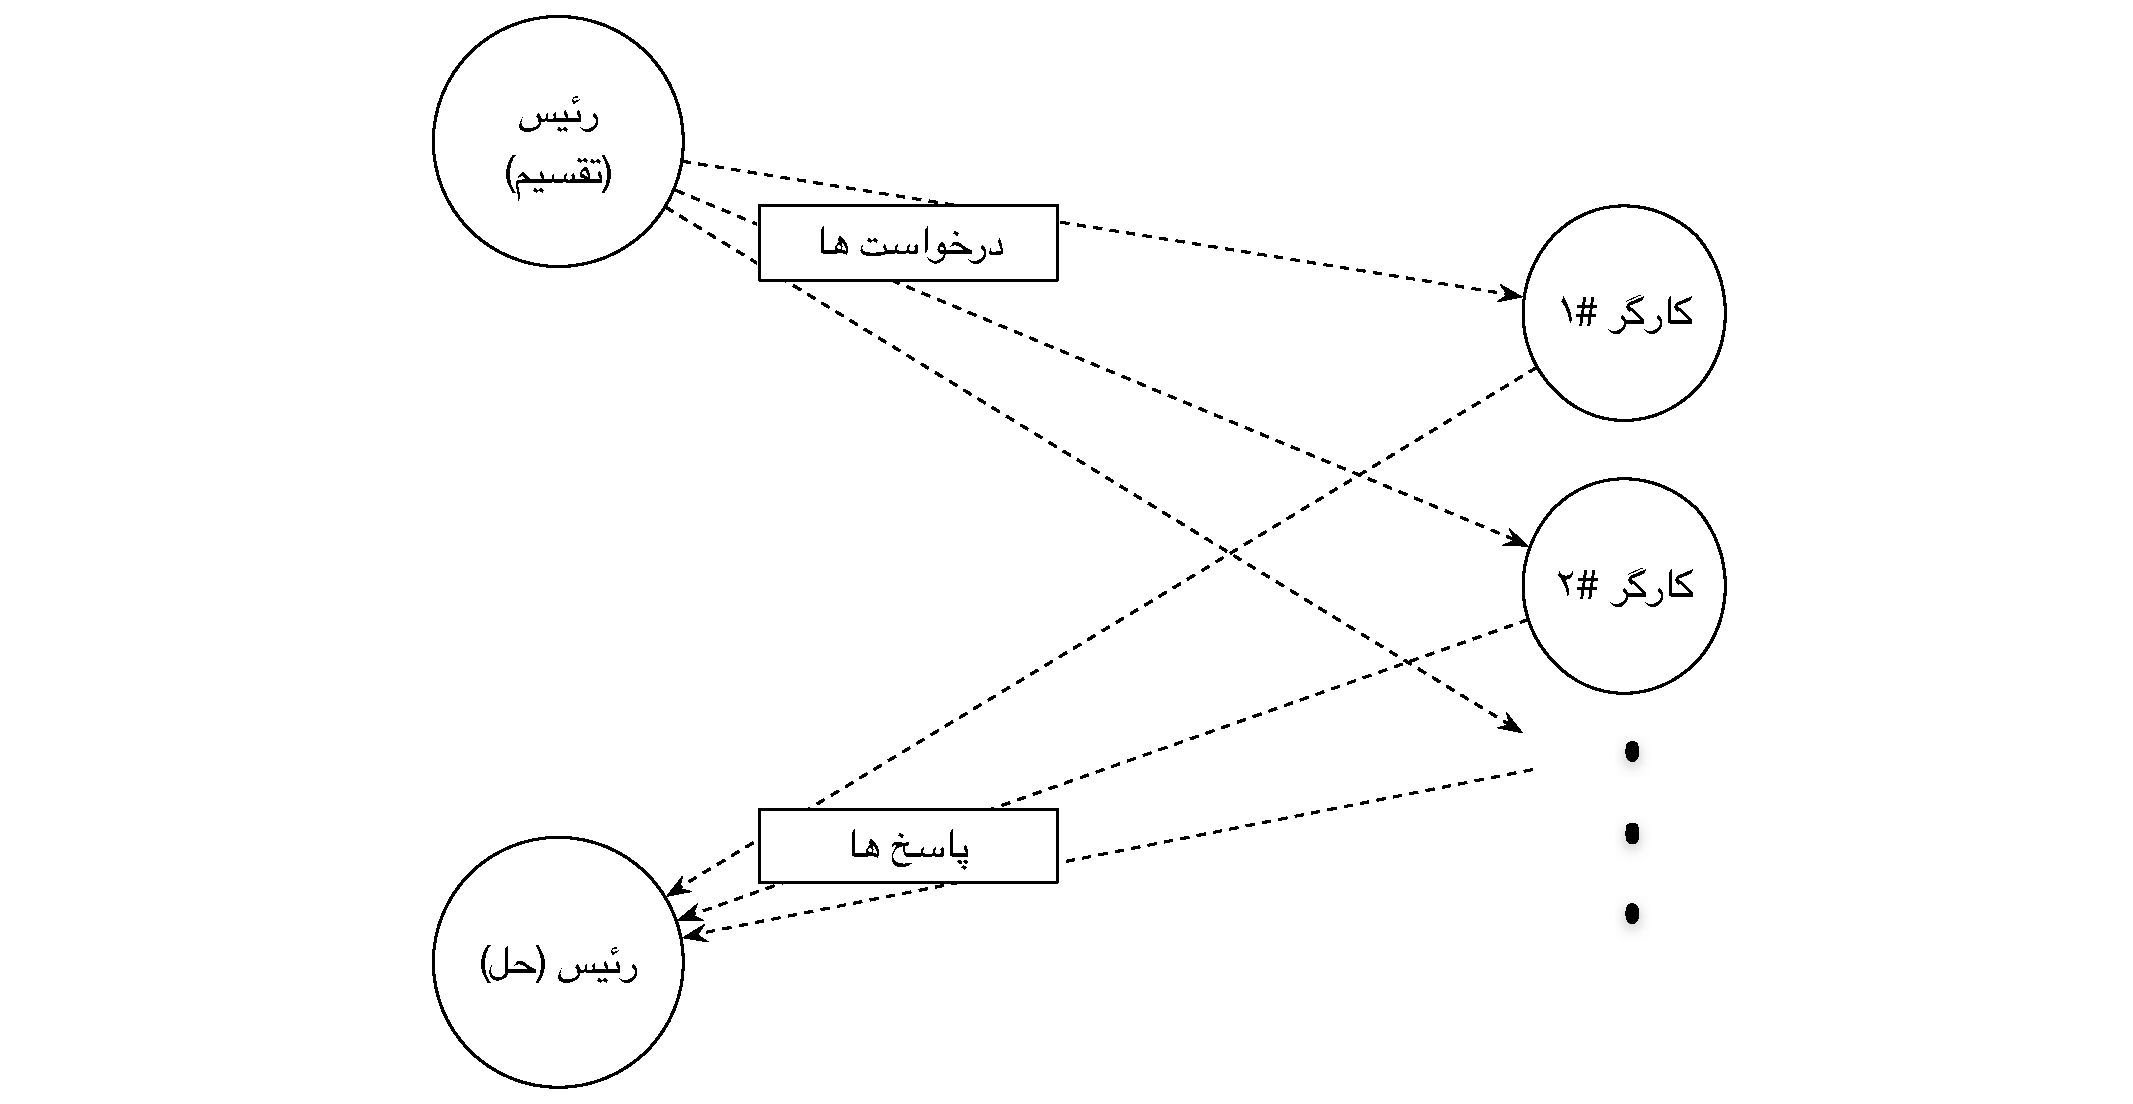
\includegraphics[width=16cm]{3-RelatedWork/Figures/Divide_and_Conquer.pdf}
    \end{center}
    \caption{\label{fig:divide_conquer}  شمای کلی از الگوی تقسیم-و-حل در مدل اکتور }
\end{figure*}
شکل \ref{fig:divide_conquer} شمایی از نحوه‌ی پیاده‌سازی الگوی تقسیم-و-حل در مدل اکتور را نمایش می‌دهد.\\
الگوی خط لوله برای حالت‌هایی مناسب است که فعالیت قابل تقسیم به بخش‌های افزایشی باشد. در این صورت هر اکتور تغییرات مربوطه را در مدل ایجاد می‌کند و آن را به عنوان پیغام به اکتور بعدی در خط لوله منتقل می‌کند.

\begin{figure*}
    \begin{center}
	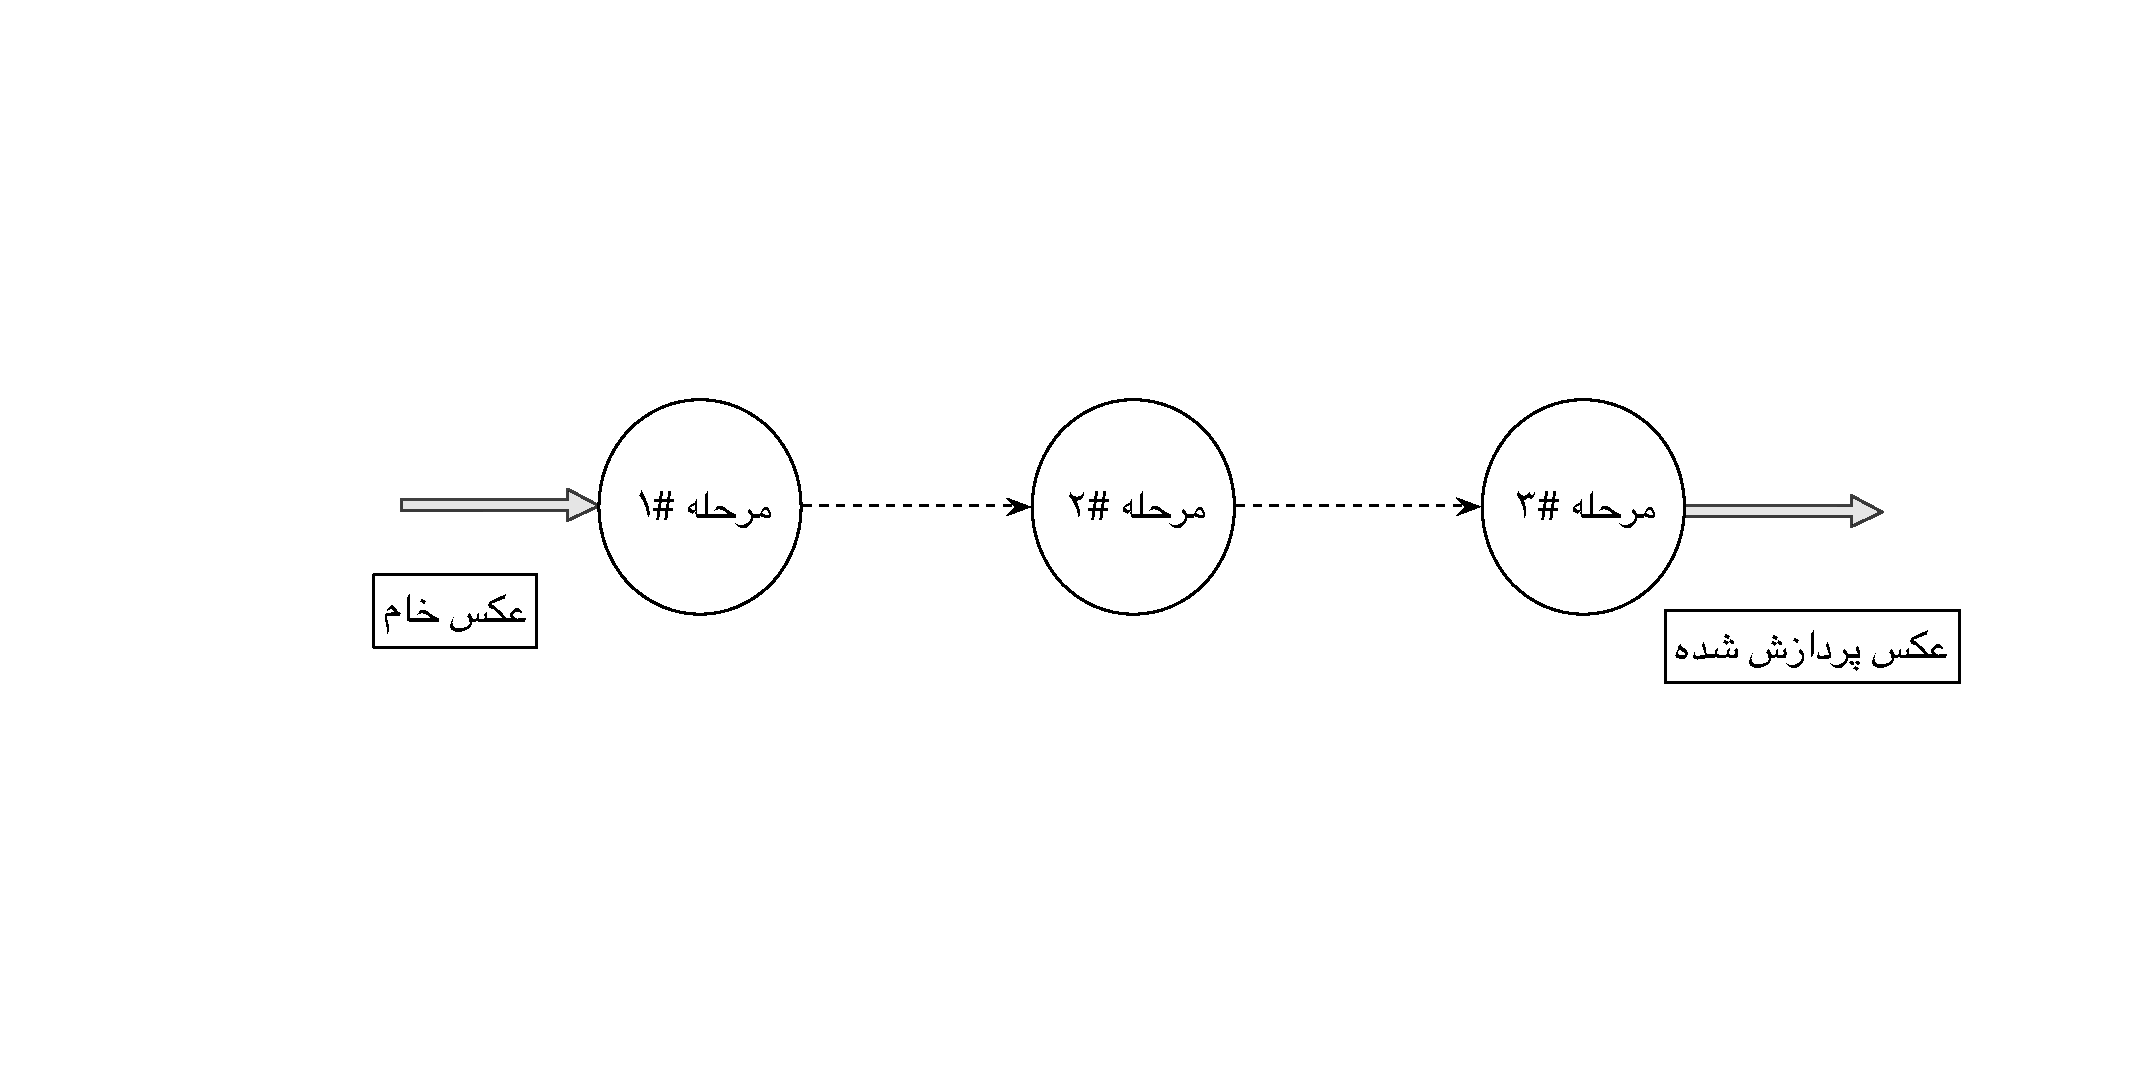
\includegraphics[width=16cm]{3-RelatedWork/Figures/pipeline.pdf}
    \end{center}
    \caption{\label{fig:pipeline}  مثالی از الگوی خط لوله (پردازش تصویر) }
\end{figure*}
به عنوان مثالی از الگوی خط لوله یک برنامه‌ی پردازش تصویر را در نظر بگیرید. هر مرحله از خط لوله، تغییراتی را در تصویر دریافتی ایجاد می‌کند و تصویر نتیجه را به مرحله‌ی بعد منتقل می‌کند. در پیاده‌سازی با روش اکتور، هر مرحله به صورت یک اکتور مدل می‌شود و تصویر به صورت پیغام بین مراحل رد و بدل می‌شود. در شکل \ref{fig:pipeline} شمایی از این الگو نشان داده شده‌ است. \\
در پژوهش‌های انجام شده مشخص شد که الگوهای ارائه شده صرفا الگوهای کلی همروندی هستند و جزئیات این الگوها در طراحی منطق دامنه، نحوه‌ی طراحی پیغام‌ها بررسی نشده اند .

\section{ همگام‌سازی و هماهنگی اکتورها }
\label{section:coordinationAndSyncronization}
همان‌طور که در بخش‌های قبل ذکر شد،  مدل اکتور دارای خاصیت ناهمگامی‌ است و ترتیب پیغام‌هایی که یک اکتور دریافت می‌کند وابسته به ترتیب فرستاده شدن پیغام‌ها نیست. نتیجه‌ی این خاصیت این است که تعداد ترتیب\LTRfootnote{ordering}‌های دریافت پیغام‌ها در مدل اکتور نمایی است\cite{KarmaniAgha_Actors_11}. به دلیل اینکه فرستنده‌ی پیغام از حالت محلی اکتور گیرنده اطلاعی ندارد، ممکن است بعضی از ترتیب‌های ذکر شده برای پیغام‌ها مطلوب نباشد. به عنوان مثال الگوریتمی را در نظر بگیرید که زیر بخش‌های مختلف آن به اکتور‌هایی فرستاده شده و نتایج آن دریافت می‌شود ولی در آن ترتیب دریافت نتایج اهمیت داشته باشد.  نیاز به این نوع اولویت‌بندی‌ها در مدل اکتور منجر به ایجاد پیچیدگی در محاسبات همروند می‌شود و در صورت پیاده‌سازی نامناسب باعث ایجاد ناکارامدی در برنامه‌ها می‌شود. راه حل این مسئله در مدل اکتور همگام‌سازی است. در مدل اکتور، اکتور‌ها برای همگام‌سازی باهم ارتباط برقرار می‌کنند. در این قسمت دو نوع الگوی هماهنگی اکتور‌ها را معرفی می‌کنیم: تبادل پیغام شبه آرپی‌سی (فراخوانی رویه راه دور)\LTRfootnote{Remote Procedure Call} و قیود همگام‌سازی محلی \LTRfootnote{Local Synchronization Constraints}. \cite{Agha1990,Agha93abstractionand,Papaioannou,KarmaniAgha_Actors_11} 
\subsection{تبادل پیغام شبه-آرپی‌سی}
در ارتباط شبه‌-آرپی‌سی، فرستنده‌ پس از ارسال پیغام منتظر گرفتن پیغام پاسخ از طرف گیرنده می‌ماند. رفتار اکتور در این مدل به ترتیب زیر است:
\begin{enumerate}
\item اکتور فرستنده درخواست را در قالب یک پیغام به اکتور گیرنده ارسال می‌کند.
\item سپس فرستنده صندوق پیغام‌ها را بررسی می‌کند.   
\item اگر پیغام بعدی پاسخ درخواست ارسال شده باشد اقدام مناسب صورت می‌گیرد و فعالیت اکتور ادامه پیدا می‌کند.
\item اگر پیغام بعدی پاسخ درخواست ارسال شده نباشد پیغام جاری در صورت امکان (بسته به منطق برنامه) پردازش می‌شود و در غیر این صورت برای پردازش در آینده به صندوق پیغام‌ها برگردانده می‌شود.
\end{enumerate}
شکل \ref{fig:rpc} مثالی از  پیاده‌سازی ارتباط شبه-آرپی‌سی در مدل اکتور را نشان می‌دهد. ارتباط شبه-آرسی‌پی در دو نوع سناریوی خاص مفید و ضروری است: یک سناریو این است که اکتور نیاز به ارسال پیغام به صورت ترتیبی به یک یا چند اکتور خاص دارد و تا حاصل شدن اطمینان از رسیدن پیغام قبلی پیغام بعد را ارسال نمی‌کند. سناریوی دوم این است که حالت\LTRfootnote{state} اکتور فرستنده بستگی به محتوای پاسخ دارد. در این حالت اکتور قبل از دریافت پاسخ مورد نظر، نمی‌تواند پیغام‌های بعدی را به درستی پردازش کند. نکته‌ی قابل توجه این است که با توجه به شباهت ارسال پیغام شبه-آرپی‌سی به فراخوانی رویه\LTRfootnote{procedure}‌ها در زبان‌های \gls{ترتیبی}\LTRfootnote{sequential}، معمولا برنامه‌نویسان گرایش به استفاده‌ی بیش از حد از این نوع تبادل پیغام دارند که این ممکن است با ایجاد وابستگی‌های بی‌مورد در اشیاء برنامه، علاوه بر کاهش کارایی، منجر به ایجاد \gls{بن‌باز}\LTRfootnote{live lock} در برنامه شود (حالتی که یک اکتور به علت انتظار برای پاسخی که هرگز دریافت نخواهد کرد، از پیغام‌های جدید مرتباً چشم‌پوشی می‌کند یا پردازش آنها را به تأخیر می‌اندازد).\\
امکان تبادل پیغام شبه-آرپی‌سی تقریبا در تمامی پیاده‌سازی‌های مدل اکتور به صورت امکانات سطح زبان وجود دارد\cite{ActorsJVM2009}.

\begin{figure*}
    \begin{center}
	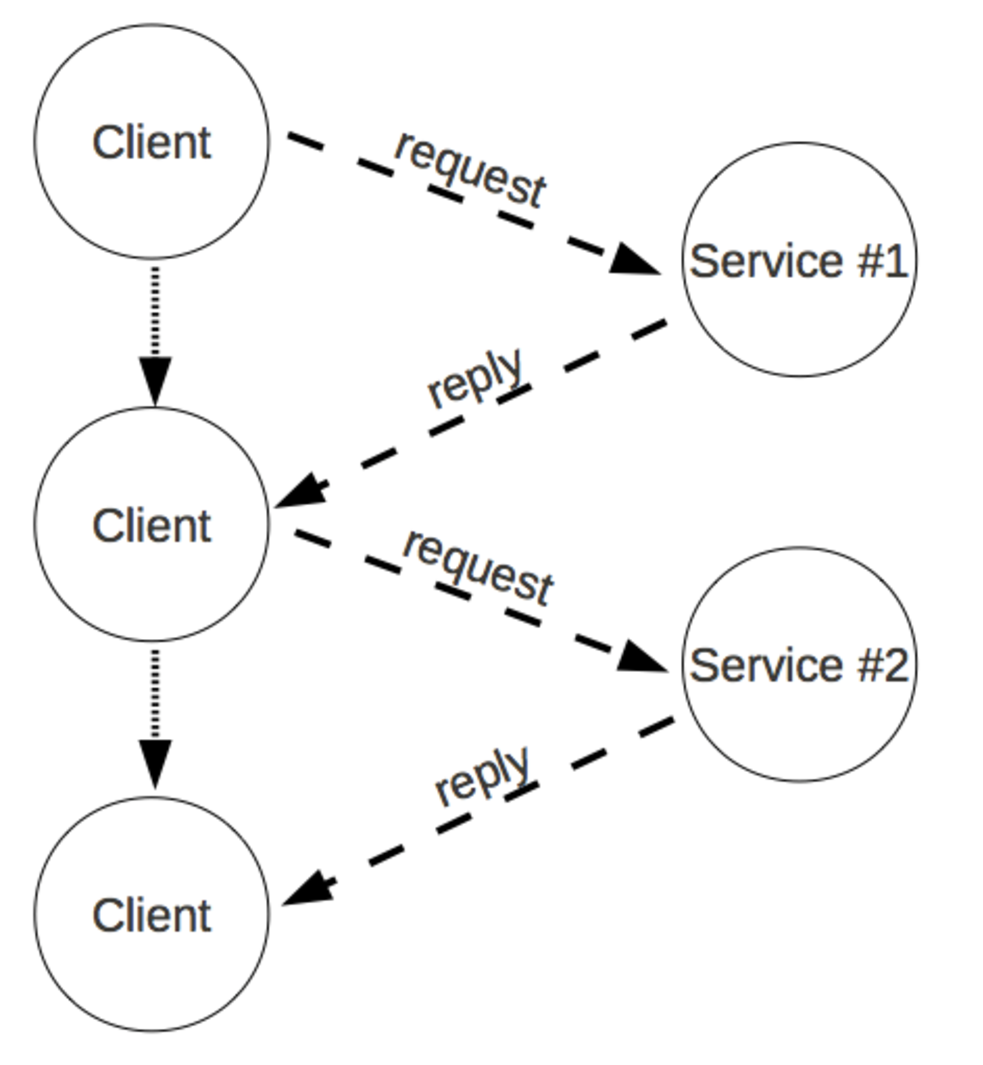
\includegraphics[width=10cm]{3-RelatedWork/Figures/RPC.pdf}
    \end{center}
    \caption{\label{fig:rpc} مثالی از ارتباط شبه-آرپی‌سی در اکتورها) }
\end{figure*}
 
\subsection{قیود همگام‌سازی محلی}
\label{subsec:local_sync_constraints}
استفاده از قیود همگام‌سازی محلی روشی برای اولیت‌بندی پردازش پیغام‌ها در مدل اکتور است\cite{FrolundCoord}. برای توضیح مفهوم همگام‌سازی محلی مثالی در شکل \ref{fig:lsc} ارائه شده است. در این مثال اکتور فایل پس از دریافت پیغام باز کردن فایل\LTRfootnote{open}، با استفاده از قیود همگام‌سازی خود را محدود به پردازش پیغام‌های \textit{بستن} , \textit{خواندن} می‌کند. در صورت عدم وجود امکانات مناسب برای قیود همگام‌سازی، برنامه‌نویس ناگزیر خواهد بود تا در میان منطق اجرای پیغام‌ها، میانگیر صندوق پیغام‌ها را بررسی و ترکیب یا ترتیب آنها را تغییر داده و یا با جستجو در آنها پیغام مناسب را انتخاب کند. این امر موجب مخلوط شدن منطق چگونگی پردازش پیغام  (چگونه) با منطق زمانی انتخاب پیغام (چه زمانی) می‌شود که در اصول نرم‌افزار پدیده‌ی نامطلوبی به حساب می‌آید\cite{KarmaniAgha_Actors_11}. به همین دلیل بسیاری از زبان‌ها و چارچوب‌های مبتنی بر اکتور امکانات مناسبی برای پشتیبانی از قیود‌ همگام‌سازی محلی ارائه داده‌اند. به عنوان مثال در کتابخانه‌ی اکتور اسکالا که در بخش \ref{section:scalaActorLib} معرفی شد، از مکانیزم تطابق الگو\LTRfootnote{pattern matching} برای اولیت بندی پردازش پیغام‌ها بدون اینکه با منطق اجرایی برنامه مخلوط گردد استفاده می‌شود.



\begin{figure*}
    \begin{center}
	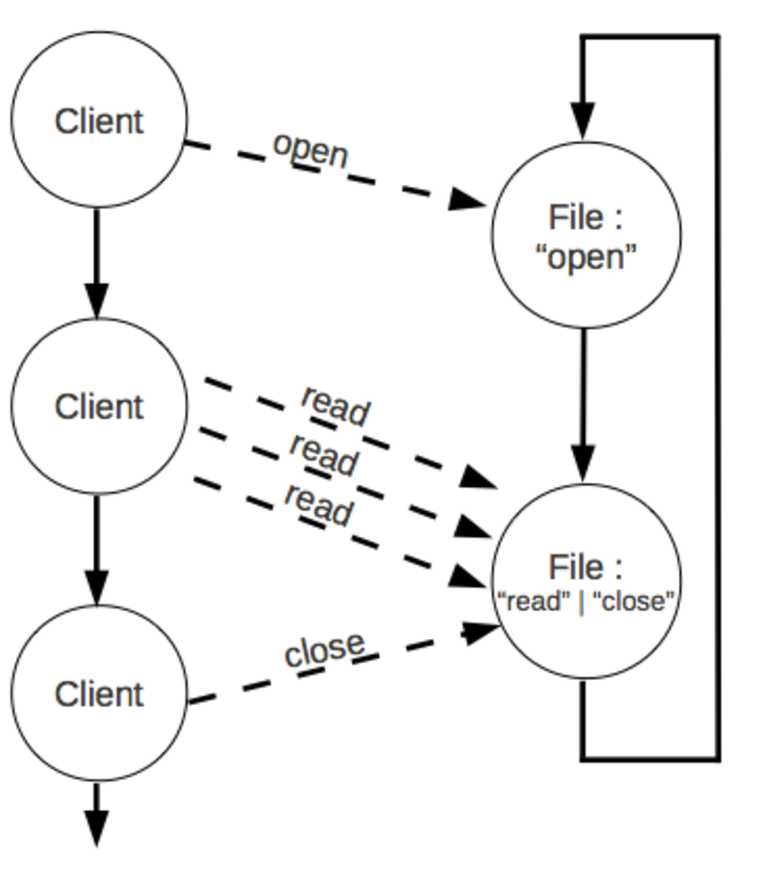
\includegraphics[width=10cm]{3-RelatedWork/Figures/LSC.pdf}
    \end{center}
    \caption{\label{fig:lsc} مثالی از قیود همگام‌سازی محلی. اکتور فایل به وسیله‌ی قیود همگام‌سازی محدود شده است. فلش عمودی به معنی ترتیب زمانی و برچسب‌های داخل دایره به معنی پیغام‌های قابل پردازش در هر حالت هستند. ) }
\end{figure*}

\chapter{طراحی بر اساس تبادل ناهمگام پیغام}
\label{chapter:proposedFramework}
\thispagestyle{plain}
\section{مقدمه}
\label{sectio:design:preface}
در این فصل از پژوهش روش طراحی منطق دامنه بر اساس تبادل ناهمگام پیغام ارائه شده است. تلاش شده است تا تطابق طراحی با مدل بازیگر در حد امکان حفظ شود. با توجه به تمرکز این بخش بر روش طراحی منطق دامنه و به هدف ایجاد شفافیت و افزایش قابلیت فهم نکات و الگوهای مطرح شده در روش، تصمیم به استفاده از یک سیستم نمونه به عنوان مثال گرفته شد. کلیه‌ی نکات مطرح شده در ادامه‌ی این بخش در قالب این مثال ارائه خواهند شد. در انتخاب سیستم نمونه نکات ذیل مورد توجه قرار گرفته‌ است:
\begin{enumerate}
\item \textbf{دامنه‌ی سیستم انتخابی:}
رده‌ی دامنه‌ی سیستم انتخاب شده به طور کلی سیستم‌های اطلاعاتی\LTRfootnote{Information System} است. اولین دلیل انتخاب این رده این است که در این نوع دامنه همروندی به طور ذاتی وجود ندارد و به همین دلیل زمینه‌ی مقایسه‌ی طراحی بر اساس تبادل ناهمگام با  طراحی‌های شیءگرای ترتیبی فراهم می‌شود. با توجه به اینکه یکی از موارد مقایسه‌ی این نوع طراحی با طراحی شیءگرای ترتیبی تفاوت کارایی این دو رویکرد است، دامنه‌ی انتخاب شده باید در حالت ترتیبی هم قابلیت اضافه شدن همروندی را داشته باشد. سیستم‌های اطلاعاتی از این حیث نیز انتخاب مناسبی محسوب می‌شوند چرا که در اکثر پیاده‌سازی‌های عملیاتی، علیرغم داشتن طراحی ترتیبی، به وسیله‌ی ریسمان‌هایی که وب‌سرورها برای پاسخگویی به درخواست‌های همزمان کاربران ایجاد می‌کنند، دارای خاصیت همروندی نیز می‌گردند. به همین دلیل در بخش ارزیابی می‌توانیم با شبیه‌سازی عملیات وب‌سرورها، کارایی و نیز تغییرپذیری دو نوع طراحی مذکور را ارزیابی و مقایسه کنیم.
 دلیل دیگر این انتخاب بالا بودن میزان آشنایی جامعه‌ی طراحی شیءگرا با این نوع سیستم‌ها و استفاده‌ی گسترده از این نوع سیستم‌ها می‌باشد. شایان ذکر است که سعی شده است در ارائه‌ی الگوها و نکات استخراج شده از این طراحی بر دامنه‌ی انتخاب شده تکیه‌ نشود. دامنه‌ی سیستم نمونه نیز یک سیستم آموزشی انتخاب شده است. با توجه به اینکه استفاده کنندگان این پژوهش جامعه‌ی دانشگاهی هستند، آشنایی این جامعه با سیستم آموزشی دلیل اصلی انتخاب آن بوده است. 
\item \textbf{ بزرگی منطق دامنه:}
از نظر میزان بزرگی سیستم (تعداد کلاس‌ها و موارد کاربرد\LTRfootnote{use cases})،‌  سعی شده منطق حداقل بزرگی و پیچیدگی را داشته باشد تا ضمن امکان مشاهده‌ی الگوهای مختلف، نیازی به تکرار نکات طراحی برای مولفه‌های متعدد و مشابه نباشد. 
\end{enumerate} 

\section{معرفی یک سیستم آموزش ساده }
\label{section:eduIntro}
همان‌طور که در بخش \ref{sectio:design:preface} ذکر شد،‌ یک سیستم آموزش کوچک به عنوان مدل طراحی انتخاب شده است. در ادامه‌ی این بخش ابتدا موارد کاربرد\LTRfootnote{use cases} انتخاب شده در این سیستم را توصیف می‌کنیم و سپس با توجه به‌ آنها مدل دامنه\LTRfootnote{Domain Model} سیستم را در قالب نمودار کلاس بیان می‌کنیم.

\subsection{موارد کاربرد}
در این بخش موارد کاربرد انتخاب شده برای سیستم آموزش معرفی می‌شوند. لازم به تأکید است که علیرغم این که این موارد کاربرد، مرتبط و هماهنگ با موارد کاربرد یک سیستم آموزش واقعی هستند، به هیچ عنوان تمام موارد کاربرد مورد نیاز برای ساختن سیستم واقعی را شامل نمی‌شوند و علاوه‌ بر آن، موارد انتخاب شده دارای جزئیات و دقت کافی برای پوشش فرایند‌های واقعی نیستند. در ادامه‌ی این بخش، هر \gls{مورد کاربرد} در قالب یک جدول توصیفی ارائه شده‌ است.


%%%%%%%%%%%%%%%%%%%%%%%%%%%%%
%%%%  GPA
%%%%%%%%%%%%%%%%%%%%%%%%%%%%%
\begin{table}
\begin{center}
\begin{tabular}{|p{5cm}|p{10cm}|}
	\hline
	\textbf{نام مورد کاربرد} &
درخواست محاسبه‌ی معدل ترم دانشجو\\
	\hline
	\textbf{بازیگر(ان)} &
کاربر\\
	\hline
	\textbf{شروع می‌شود زمانی که} &
درخواست محاسبه‌ی معدل ترم وارد سیستم می‌شود.\\
	\hline
	\textbf{پیش‌شرط‌ها} &
دانشجو و ترم در سیستم تعریف شده باشند.\\
	\hline
	\textbf{جریان اصلی} &
۱. درخواست محاسبه‌ی معدل دانشجو در ترم مربوطه وارد سیستم می‌شود.\newline
۲. سیستم سوابق تحصیلی دانشجو در ترم مربوطه را بررسی ‌می‌کند. معدل ترم با توجه به نمرات اخذ شده و تعداد واحد هر درس محاسبه و اعلام می‌شود. در صورتی که نمره‌ی درس سابقه‌ای وارد نشده باشد، درس مربوطه در محاسبه‌ی معدل لحاظ نمی‌گردد.\\
	\hline
\textbf{جریان استثنا ۱} &
۲.الف) در صورتی که دانشجو هیچ واحدی در ترم جاری اخذ نکرده باشد پیغام خطای مناسب صادر می‌شود و جریان اصلی خاتمه می‌یابد.\\
	\hline
%	\textbf{جریان استثنا ۲} &
%۴-ج. رمز وارد شده نامعتبر است، پیام خطای رمز نامعتبر است به کاربر نمایش داده شده و تراکنش متوقف می‌شود\\
%	\hline
	\textbf{تمام می‌شود زمانی که} &
معدل دانشجو اعلام می‌شود یا خطای مناسب صادر می‌گردد.\\
	\hline
%	\textbf{پس شرط‌ها} &
%کاربر موجودی کارت و یا خطای تراکنش را مشاهده کرده است.\\
%	\hline
\end{tabular}
\caption{\label{table:uc_gpa} توصیف مورد کاربرد محاسبه‌ی معدل یک دانشجو در یک ترم}
\end{center}
\end{table}

%%%%%%%%%%%%%%%%%%%%%%%%%%%%%
%%%%  Take Course
%%%%%%%%%%%%%%%%%%%%%%%%%%%%%
\begin{table}
\begin{center}
\begin{tabular}{|p{4cm}|p{12cm}|}
	\hline
	\textbf{نام مورد کاربرد} &
درخواست اخذ یک ارائه در یک ترم\\
	\hline
	\textbf{بازیگر(ان)} &
کاربر\\
	\hline
	\textbf{شروع می‌شود زمانی که} &
درخواست اخذ ارائه وارد سیستم می‌شود.\\
	\hline
	\textbf{پیش‌شرط‌ها} &
۱. ‌انتخاب واحد در ترم امکانپذیر باشد. (رجوع کنید به جداول \ref{table:uc_enableofferings}و\ref{table:uc_disableofferings})\\
	\hline
	\textbf{جریان اصلی} &
۱. سیستم کنترل می‌کند که دانشجو در ترم‌های قبل این درس را نگذرانده باشد.\newline
۲. سیستم کنترل می‌کند که دانشجو در ترم‌ جاری این درس را اخذ نکرده باشد.\newline
۳. سیستم کنترل می‌کند که دانشجو تمام پیش‌نیاز‌های این درس را با موفقیت گذرانده باشد.\newline
۴. سیستم کنترل می‌کند که تعداد واحد‌های اخذ شده توسط دانشجو در این ترم پس از اخذ این درس بیشتر از ۲۰ نشود.\newline
۵. سیستم یک سابقه از ارائه‌ی انتخاب شده برای دانشجو تشکیل می‌دهد و آن را در سوابق دانشجو ثبت می‌کند.\\
	\hline
\textbf{جریان استثنا ۱} &
۱.الف)در صورتی که دانشجو قبلا این درس را گذرانده باشد، خطای ''درس انتخاب شده قبلاً گذرانده شده است`` صادر می‌شود و جریان اصلی خاتمه می‌یابد.\\
	\hline
\textbf{جریان استثنا ۲} &
۲.الف)در صورتی که دانشجو در ترم جاری این درس را اخذ کرده باشد، خطای ''این درس در ترم جاری قبلاً اخذ شده است`` صادر می‌شود و جریان اصلی خاتمه می‌یابد.\\
	\hline
\textbf{جریان استثنا ۳} &
۳.الف)در صورتی که دانشجو یکی از پیش‌نیاز‌های درس‌ را نگذرانده باشد، خطای ''انتخاب بیشتر از ۲۰ واحد در ترم مجاز نمی‌باشد`` صادر می‌شود و جریان اصلی خاتمه می‌یابد.\\
	\hline
\textbf{جریان استثنا ۴} &
۴.الف)در صورتی که تعداد واحد‌های اخذ شده توسط دانشجو در این ترم پس از اخذ این درس بیشتر از ۲۰ شود، خطای ''انتخاب بیشتر از ۲۰ واحد در ترم مجاز نمی‌باشد`` صادر می‌شود و جریان اصلی خاتمه می‌یابد.\\
	\hline
	\textbf{تمام می‌شود زمانی که} &
سابقه‌ی جدید در سوابق دانشجو ثبت می‌شود و یا خطای مناسب صادر می‌گردد.\\
	\hline
\end{tabular}
\caption{\label{table:uc_takecoure} توصیف مورد کاربرد اخذ یک ارائه توسط یک دانشجو در یک ترم}
\end{center}
\end{table}

%%%%%%%%%%%%%%%%%%%%%%%%%%%%%
%%%%  DISABLE_TERM_OFFERINGS
%%%%%%%%%%%%%%%%%%%%%%%%%%%%%
\begin{table}
\begin{center}
\begin{tabular}{|p{5cm}|p{10cm}|}
	\hline
	\textbf{نام مورد کاربرد} &
درخواست غیر فعال کردن ارائه‌های یک ترم برای انتخاب واحد\\
	\hline
	\textbf{بازیگر(ان)} &
کاربر(مدیر سیستم)\\
	\hline
	\textbf{شروع می‌شود زمانی که} &
درخواست غیرفعال کردن ارائه‌های یک ترم وارد سیستم می‌شود.\\
	\hline
	\textbf{پیش‌شرط‌ها} &
 ترم در سیستم تعریف شده باشند.\\
	\hline
	\textbf{جریان اصلی} &
۱. درخواست غیر فعال کردن ارائه‌های یک ترم وارد سیستم می‌شود.\newline
۲.سیستم تمام ارائه‌های یک ترم را غیرفعال می‌کند.\\
	\hline
	\textbf{تمام می‌شود زمانی که} &
تمام ارائه‌های ترم برای انتخاب واحد غیرفعال می‌شوند.\\
	\hline
	\textbf{پس شرط‌ها} &
انتخاب واحد در ترم امکان پذیر نیست.\\
	\hline
\end{tabular}
\caption{\label{table:uc_disableofferings} توصیف مورد کاربرد غیرفعال کردن ارائه‌های یک ترم برای انتخاب واحد}
\end{center}
\end{table}

%%%%%%%%%%%%%%%%%%%%%%%%%%%%%
%%%%  ENABLE_TERM_OFFERINGS
%%%%%%%%%%%%%%%%%%%%%%%%%%%%%
\begin{table}
\begin{center}
\begin{tabular}{|p{5cm}|p{10cm}|}
	\hline
	\textbf{نام مورد کاربرد} &
درخواست فعال کردن ارائه‌های یک ترم برای انتخاب واحد\\
	\hline
	\textbf{بازیگر(ان)} &
کاربر(مدیر سیستم)\\
	\hline
	\textbf{شروع می‌شود زمانی که} &
درخواست فعال کردن ارائه‌های یک ترم وارد سیستم می‌شود.\\
	\hline
	\textbf{پیش‌شرط‌ها} &
 ترم در سیستم تعریف شده باشند.\\
	\hline
	\textbf{جریان اصلی} &
۱. درخواست فعال کردن ارائه‌های یک ترم وارد سیستم می‌شود.\newline
۲.سیستم تمام ارائه‌های یک ترم را فعال می‌کند.\\
	\hline
	\textbf{تمام می‌شود زمانی که} &
تمام ارائه‌های ترم برای انتخاب واحدفعال می‌شوند.\\
	\hline
	\textbf{پس شرط‌ها} &
انتخاب واحد در ترم امکان پذیر است.\\
	\hline
\end{tabular}
\caption{\label{table:uc_enableofferings} توصیف مورد کاربرد فعال کردن ارائه‌های یک ترم برای انتخاب واحد}
\end{center}
\end{table}


\subsection{اشیاء دامنه}
\label{subsec:mainEntities}
 موجودیت‌های اصلی  مدل ابتدایی این سیستم عبارتند از:
\textbf{\textit{دانشجو}}\LTRfootnote{Student}، \textbf{\textit{درس}}\LTRfootnote{Course}، \textbf{\textit{ترم}}\LTRfootnote{Term}، \textbf{\textit{ارائه}}\LTRfootnote{Offering} و \textbf{\textit{سابقه}}\LTRfootnote{Study Record}.\\
در هر \textit{ترم} تحصیلی، تعدادی \textit{ارائه} از دروس مختلف وجود دارد. هر درس می‌تواند \textit{ارائه}های مختلفی داشته باشد. به عنوان مثال درس ریاضی۱ می‌تواند در ترم ۹۰-۹۱-۱سه ارائه‌ی مختلف داشته باشد. دانشجو با اخذ هر ارائه \textit{سابقه}‌ای از آن ارائه را به اسم خود ثبت می‌کند. در این سابقه اطلاعاتی مثل نمره‌ی دانشجو و وضعیت قبول یا مردودی درس در طول ترم ثبت خواهد شد. دروس می‌توانند رابطه‌ی پیش‌نیازی\LTRfootnote{prerequisite} باهم داشته باشند. 
\begin{figure*}
    \begin{center}
	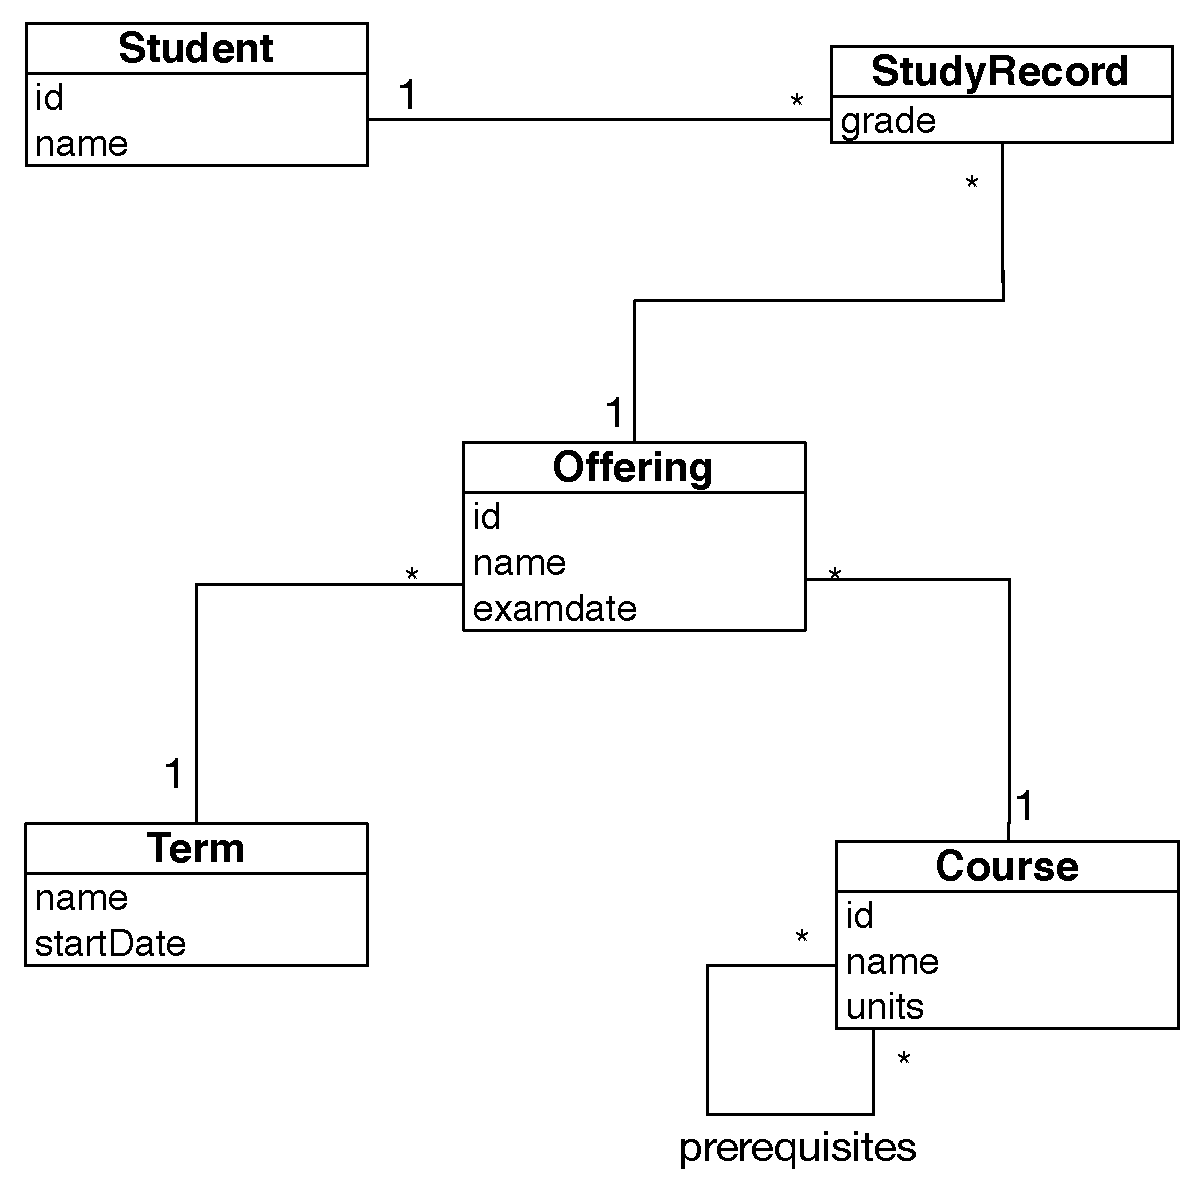
\includegraphics[width=12cm]{4-ProposedFramework/Figures/SimpleClassDiagram.pdf}
    \end{center}
    \caption{\label{fig:edu_class1} نمودار کلاس مدل ابتدای سیستم آموزش ساده }
\end{figure*}
شکل \ref{fig:edu_class1} مدل دامنه‌ی سیستم را به وسیله‌ی یک نمودار کلاس مبتنی بر \textbf{یو‌ام‌ال}\LTRfootnote{UML} نشان می‌دهد.

\newpage
\section{طراحی سیستم آموزش به روش تبادل ناهمگام پیغام}
در این بخش طراحی سیستم معرفی شده در بخش \ref{section:eduIntro} به روش تبادل ناهمگام پیغام ارائه می‌گردد. سعی شده است تا به جای ارائه‌ی یکباره‌ی طراحی نهایی، یک رویکرد \gls{افزایشی}\LTRfootnote{incremental} برای طراحی اتخاذ شود. در این رویکرد مراحل تشکیل نهایی طرح و حتی اقدامات اشتباهی که در طول طراحی برداشته شده است ارائه خواهد شد. به  این ترتیب علاوه بر قابل استفاده‌تر بودن پژوهش به صورت یک دستورالعمل \LTRfootnote{receipe} طراحی، قابلیت فهم روش طراحی هم بالاتر می‌رود.
\subsection{طراحی اکتور‌های مدل دامنه}
اکتورهای اصلی سیستم همان اشیاء مدل دامنه هستند که در بخش \ref{subsec:mainEntities} معرفی شدند.البته احتمالاً علاوه بر این اکتورها، اکتورهای دیگری نیز برای پیاده‌سازی کارکردهای سیستم استفاده خواهند شد. در طراحی اکتورهای اصلی صرفا فیلد‌های داده‌ای اکتور و نیز پیغام‌های اصلی که از روابط موجود در نمودار کلاس \ref{fig:edu_class1} قابل استخراج هستند در نظر گرفته ‌می‌شود. منطق پیاده‌سازی عملیات هر پیغام و  پیغام‌های دیگری که به این منظور ایجاد می‌شوند در ادامه به طراحی افزوده خواهد شد. 
با توجه به اینکه در مدل اکتور،‌ تنها راه ارتباط بین اکتور‌ها استفاده از تبادل پیغام است و این که یک اکتور برای امکان ارسال پیغام به اکتور دیگر نیاز به دسترسی به اسم آن دارد، بهترین راه برای طراحی رابطه‌های وابستگی\LTRfootnote{association} این است که در کلاس یک اکتور برای هر کلاس دیگر که رابطه‌ای با آن وجود دارد یک فیلد از نوع کلاس طرف دیگر در نظر گرفته شود. این مورد مشابه طراحی شیءگرای عادی (ترتیبی) است. از طرف دیگر در مدل طراحی شیءگرای ترتیبی برای هر کارکرد اصلی یک شیء نیز یک متد در کلاس متناظر با آن در نظر گرفته می‌شود که برای اجرای کارکرد، متد مورد نظر فراخوانی می‌شود. با توجه به اینکه در مدل اکتور مکانیزم کنترلی برنامه به جای فراخوانی متد، تبادل پیغام است، باید به ازای هر متد متناظر در حالت شیءگرا، یک پیغام دریافت شود. البته در این مرحله از طراحی منطق پیاده‌سازی کارکرد هر پیغام در نظر گرفته نشده است و در مراحل بعدی به تدریج اضافه خواهد شد.
\begin{enumerate}
%%%%%%%%%%%%%%%%%%%%%%%%%%%%%%%%%
%										Student												%
%%%%%%%%%%%%%%%%%%%%%%%%%%%%%%%%%
\item\textbf{اکتور دانشجو:}
این اکتور دارای فیلد‌های نام و شناسه است. به علت ارتباط دانشجو با سابقه‌ها و نیاز  به ارسال پیغام به آنها یک فیلد از نوع لیست سابقه نیز در کلاس دانشجو وجود دارد. قطعه کد \ref{fig:mainActors:student} طرح ابتدایی کلاس اکتور دانشجو را نشان می‌دهد. همان‌طور که در بخش قبل ذکر شد منطق پیاده‌سازی کارکرد پیغام‌ها در این مرحله اضافه نشده و در ادامه‌ی فصل به تدریج تکمیل خواهد شد. پیغام‌هایی که اکتور دانشجو دریافت می‌کند عبارتند از:
\begin{enumerate}
%\item\textbf{:\lr{HasPassed(course)}}
%با دریافت این پیغام اکتور دانشجو باید پاسخ بدهد که آیا درس مربوطه را گذرانده است یا خیر.
%\item\textbf{:\lr{HasTaken(course)}}
%با دریافت این پیغام دانشجو باید پاسخ دهد که در ترم جاری این درس را اخذ کرده است یا خیر.
\item\textbf{:\lr{GPARequest(term)}}
با دریافت این پیغام دانشجو باید پاسخ دهد که معدل دانشجو در ترم جاری  چند بوده است.
\item\textbf{:\lr{TakeCourse(offering)}}
با دریافت این پیغام دانشجو باید درس ارائه‌ی مربوطه را اخذ کند. طبیعتاً تمام شرایط ذکر شده در مورد کاربرد \ref{table:uc_takecoure} باید بررسی شود.
\end{enumerate}
طبیعتاً این موارد تنها شامل پیغام‌هایی است که مستقیماً از موارد کاربرد قابل استخراج هستند. در هنگام طراحی کارکردهای موارد کاربرد، در صورت لزوم پیغام‌های جدیدی به این کلاس اضافه خواهد شد.
\codelisting[language=scala]{4-ProposedFramework/src/mainActors/Student.scala}{ساختار کلاس اکتور دانشجو}{fig:mainActors:student}
%%%%%%%%%%%%%%%%%%%%%%%%%%%%%%%%%
%										StudyRecord										%
%%%%%%%%%%%%%%%%%%%%%%%%%%%%%%%%%
\item\textbf{اکتور سابقه:}
مطابق مدل دامنه‌ که در شکل \ref{fig:edu_class1} ارائه شده است، تنها فیلد داده‌ای این اکتور، نمره است. به علت ارتباط سابقه با اکتور ارائه، یک فیلد از نوع ارائه نیز در کلاس سابقه وجود دارد. قطعه کد \ref{fig:mainActors:studyrecord} طرح ابتدایی کلاس اکتور سابقه را نشان می‌دهد. همان‌طور که در بخش قبل ذکر شد منطق پیاده‌سازی کارکرد پیغام‌ها در این مرحله اضافه نشده و در ادامه‌ی فصل به تدریج تکمیل خواهد شد. در این مرحله، پیغامی که مستقیماً از موارد کاربرد قابل استخراج باشد وجود ندارد
و در هنگام طراحی کارکردهای موارد کاربرد، در صورت لزوم پیغام‌های جدیدی به این کلاس اضافه خواهد شد.
\codelisting[language=scala]{4-ProposedFramework/src/mainActors/StudyRecord.scala}{ساختار کلاس اکتور سابقه}{fig:mainActors:studyrecord}
%%%%%%%%%%%%%%%%%%%%%%%%%%%%%%%%%
%										Offering										%
%%%%%%%%%%%%%%%%%%%%%%%%%%%%%%%%%
\item\textbf{اکتور ارائه:}
مطابق مدل دامنه‌ که در شکل \ref{fig:edu_class1} ارائه شده است، فیلدهای داده‌ای این اکتور عبارتند از شناسه و تاریخ امتحان\LTRfootnote{examDate}. به علت ارتباط ارائه با اکتور‌های درس و ترم، یک فیلد از نوع درس و یک فیلد از نوع ترم نیز در کلاس ارائه وجود دارد. قطعه کد \ref{fig:mainActors:offering} طرح ابتدایی کلاس اکتور ارائه را نشان می‌دهد. در این مرحله، پیغامی که مستقیماً از موارد کاربرد قابل استخراج باشد وجود ندارد
و در هنگام طراحی کارکردهای موارد کاربرد، در صورت لزوم پیغام‌های جدیدی به این کلاس اضافه خواهد شد.
\codelisting[language=scala]{4-ProposedFramework/src/mainActors/Offering.scala}{ساختار کلاس اکتور ارائه}{fig:mainActors:offering}



%%%%%%%%%%%%%%%%%%%%%%%%%%%%%%%%%
%										Course										%
%%%%%%%%%%%%%%%%%%%%%%%%%%%%%%%%%
\item\textbf{اکتور درس:}
مطابق مدل دامنه‌ که در شکل \ref{fig:edu_class1} ارائه شده است، فیلدهای داده‌ای این اکتور عبارتند از شناسه، نام و تعداد واحد. تنها ارتباط این کلاس که نیاز به ایجاد فیلد دارد ارتباط دروس پیش‌نیاز است. بنابراین یک فیلد از نوع لیست درس نیز به این منظور باید به کلاس اضافه شود. قطعه کد \ref{fig:mainActors:course} طرح ابتدایی کلاس اکتور درس را نشان می‌دهد. در این مرحله، پیغامی که مستقیماً از موارد کاربرد قابل استخراج باشد وجود ندارد
و در هنگام طراحی کارکردهای موارد کاربرد، در صورت لزوم پیغام‌های جدیدی به این کلاس اضافه خواهد شد.
\codelisting[language=scala]{4-ProposedFramework/src/mainActors/Course.scala}{ساختار کلاس اکتور درس}{fig:mainActors:course}
%%%%%%%%%%%%%%%%%%%%%%%%%%%%%%%%%
%										Term										%
%%%%%%%%%%%%%%%%%%%%%%%%%%%%%%%%%
\item\textbf{اکتور ترم:}
مطابق مدل دامنه‌ که در شکل \ref{fig:edu_class1} ارائه شده است، فیلدهای داده‌ای این اکتور عبارتند از نام و تاریخ شروع{startDate}. با توجه به موارد کاربرد مطرح شده، اکتور ترم آغاز کننده‌ی هیچ ارتباطی نیست و به همین دلیل نیازی به داشتن فیلدی برای این منظور نیست. اکتور ترم قطعه کد \ref{fig:mainActors:term} طرح ابتدایی کلاس اکتور ترم را نشان می‌دهد. در این مرحله، پیغامی که مستقیماً از موارد کاربرد قابل استخراج باشد وجود ندارد
و در هنگام طراحی کارکردهای موارد کاربرد، در صورت لزوم پیغام‌های جدیدی به این کلاس اضافه خواهد شد.
\codelisting[language=scala]{4-ProposedFramework/src/mainActors/Term.scala}{ساختار کلاس اکتور ترم}{fig:mainActors:term}
\end{enumerate}
\newpage
\subsection{مورد کاربرد محاسبه‌ی معدل}
این مورد کاربرد در جدول \ref{table:uc_gpa} توصیف شده است. 
\subsubsection{رویکرد اول}
\label{gpa_approach1}
برای محاسبه‌ی معدل ترم یک دانشجو نیاز داریم نمره‌ی تمام درس‌های دانشجو در ترم به همراه تعداد واحد‌های آن درس‌ها را در اختیار داشته باشیم. درخواست معدل برای ترم از طرف دانشجو صورت می‌گیرد بنابراین شروع پیغام‌ها از این اکتور آغاز می‌شود.
 اکتور دانشجو به هر کدام از اکتور‌های سابقه\LTRfootnote{StudyRecord} یک پیغام می‌فرستد و به وسیله‌ی آن اعلام می‌کند نمره و تعداد واحد‌های درس مربوط به سابقه در پاسخ ارسال شود. علاوه بر این، در پاسخ باید مشخص شود که آیا سابقه‌ مربوط به همان ترم است که معدل برای آن درخواست شده یا خیر. بنابراین پیغام‌های  درخواست نمره برای معدل و پاسخ آن به صورت زیر خواهند بود:
\begin{latin}
 \begin{description}
 \item[\lr{request: GPAInfoRequest( term: Term)}]
  \item[\lr{response: GPAInfoResponse(isForTerm:Boolean, grade: Double, units:Int)}]
 \end{description}
 \end{latin}
  اکتور سابقه امکان اینکه بدون برقراری ارتباط با اکتور ارائه\LTRfootnote{Offering} جواب این پیغام را بدهد، ندارد. دلیل این امر این است که اولا سابقه‌ لزوما مربوط به ترمی نیست که معدل برای آن درخواست شده است، ثانیا سابقه اطلاعی از تعداد واحد‌های درس مربوطه ندارد. به همین دلیل، سابقه باید برای جمع‌آوری این اطلاعات با اکتورهای دیگر تبادل پیغام انجام دهد. از طرف دیگر تنها اکتوری که به نمره‌ی دانشجو دسترسی ادارد، اکتور سابقه است. در نتیجه فرستادن پاسخ به درخواست دانشجو نیاز به همکاری ۳ اکتور سابقه، درس و ترم دارد. با توجه به اینکه دسترسی سابقه به اکتورهای درس و ترم از طریق اکتور ارائه ممکن می‌شود، این اکتور نیز در تبادل پیغام‌ها مشارکت خواهد داشت.\\
با توجه به موارد ذکر شده، اکتور سابقه دو راهکار پیش رو دارد:
\begin{enumerate}
\item اکتور سابقه به وسیله‌ی درخواست‌هایی، تعیین کند که ترم مربوط به این سابقه همان ترم مورد درخواست در معدل است یا خیر، و نیز تعداد واحد‌های درس چند است. و  در ادامه با ترکیب این اطلاعات با نمره‌ی سابقه، خود پاسخ اکتور دانشجو را ارسال کند.
\item اکتور سابقه نمره را در پاسخ قرار دهد ولی با توجه به اینکه پاسخ هنوز کامل نیست (هنوز معلوم نیست که درس چند واحدی است و آیا مربوط به ترم درخواستی است یا خیر)، به جای اینکه پاسخ را برای دانشجو پس بفرستد، آن را برای تکمیل به اکتور ارائه منتقل کند.
\end{enumerate} 
در این رویکرد فرض بر انتخاب اول است، یعنی اینکه خود اکتور سابقه، با گرفتن اطلاعات مورد نیاز از ارائه، پاسخ دانشجو را ارسال می‌کند.\\
برای این کار اکتور سابقه پیغام GPAInfoRequest را برای اکتور ارائه ارسال می‌کند و منتظر دریافت پاسخ می‌ماند. اکتور ارائه با دریافت GPAInfoRequest دو پیغام به صورت زیر به ترتیب برای اکتور ترم و اکتور درس ارسال می‌کند و منتظر پاسخ آنها می‌ماند:
\begin{latin}
 \begin{description}
 \item[\lr{IsYourTermRequest(term: Term)}]
  \item[\lr{NumOfUnitsRequest}]
 \end{description}
 \end{latin}
هدف از درخواست اول این است که مشخص شود که  درسی که سابقه به آن متعلق است، متعلق به همان ترمی است که معدل برای‌ آن درخواست شده یا خیر (اگر جواب خیر باشد نمره‌ی درس در معدل در نظر گرفته نخواهد شد). پیغام دوم هم تعداد واحد‌های درس را از اکتور درس درخواست می‌کند. ترم و درس به سادگی به این دو پیغام پاسخ می‌دهند و ارائه با گرفتن پاسخ‌ها، اطلاعات آنها را تجمیع\footnote{منظور از تجمیع در اینجا این است که  پاسخ فرضی true برای پیغام \lr{IsYourTermRequest(term)} و پاسخ فرضی 3 برای پیغام \lr{NumOfUnitsRequest} را که به ترتیب از اکتورهای ترم و درس گرفته شده، به صورت پیغام \lr{GPAInfoResponse(isForTerm=true,grade=null,unit=3)} باهم ترکیب می‌کند.} کرده و برای اکتور سابقه ارسال می‌کند.  سابقه با دریافت این پیغام، به تمام اطلاعات لازم برای این که پاسخ اکتور دانشجو را بدهد، دسترسی دارد. بنابراین می‌تواند با اضافه کردن مقدار فیلد نمره‌ی خود به پیغام آن را برای دانشجو ارسال کند. دانشجو با گرفتن این پاسخ، یکی از نمره‌های لازم برای محاسبه‌ی معدل را در دست دارد. بقیه‌ی نمره‌ها از تکرار همین عملیات برای تمام اکتورهای سابقه‌ی مربوط به دانشجو به طور مشابه به دست می‌آیند. در نهایت اکتور دانشجو با جمع نمراتی که مربوط به ترم درخواستی بوده‌اند (که از مقدار فیلد isForTerm از پیغام‌های پاسخ قابل تشخیص است) و تقسیم آن بر جمع واحد‌های مربوط به ترم (فیلد units پیغام پاسخ) معدل را محاسبه کرده و برای اکتوری که درخواست معدل داده ارسال می‌کند.
   شکل \ref{fig:gpa1_sequence} نمودار ترتیب\LTRfootnote{sequence diagram} برای پیغام‌های مبادله شده در این رویکرد را در قالب یک مثال نشان می‌دهد. در بخشی از این مثال که در شکل قابل مشاهده است فرض شده ترم مربوط به درخواست معدل باشد و تعداد واحد‌های درس ۳ باشد. نمره‌ی سابقه‌ای که درخواست برای آن ارسال شده ۱۲ است. درنهایت پس از تکرار حلقه‌ی مشخص شده در شکل و ارسال پیغام‌‌ها به تمام سابقه‌ها عدد فرضی ۱۵/۲۵ به عنوان معدل محاسبه شده و به صورت پیغام ارسال شده است. لازم به ذکر است که در این شکل برای سادگی نمایش فرض شده که تکرارهای حلقه برای سابقه‌های مختلف انجام شده است و طبیعتا استاندارد یو‌ام‌ال برای آن به طور کامل رعایت نشده است.

\begin{figure*}
    \begin{center}
	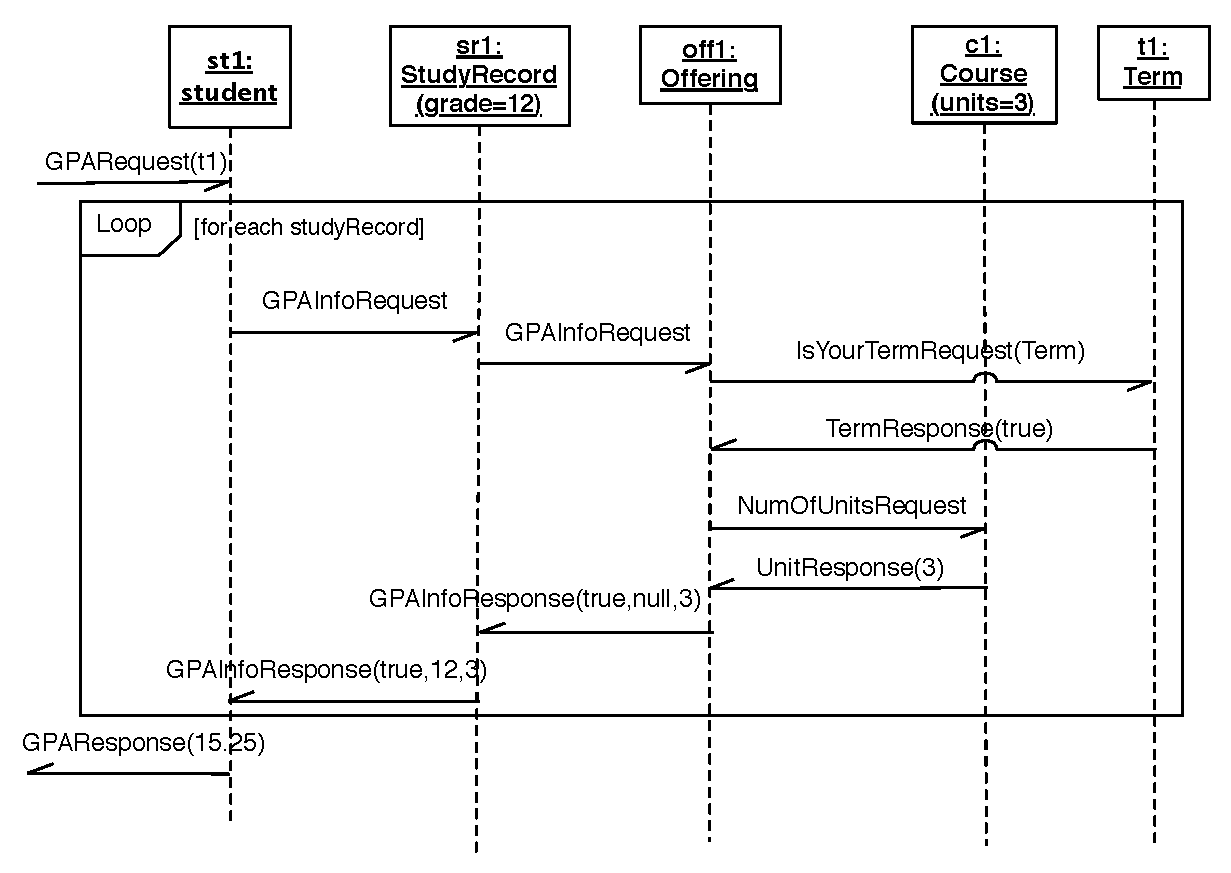
\includegraphics[width=16cm]{4-ProposedFramework/Figures/gpa_1_sequence.pdf}
    \end{center}
    \caption{\label{fig:gpa1_sequence} نمودار ترتیب برای رویکرد اول محاسبه‌ی معدل }
\end{figure*}
\FloatBarrier
در این بخش از طراحی لازم است به دو پرسش مهم پاسخ دهیم:\\
پرسش اول این است که در هر کدام از قسمت‌های طراحی که یک اکتور پیغام را فرستاده و منتظر جواب می‌ماند، آیا اکتور می‌تواند در طول مدت انتظار به فعالیت‌های دیگربپردازد؟ به عبارت بهتر، \textbf{آیا ارسال پیغام‌ها به صورت همگام است یا ناهمگام؟}\\
پرسش دوم این است که در صورتی که ارسال پیغام ناهمگام باشد ادامه‌ی فعالیت اکتور به چه صورتی مجاز است؟ آیا می‌تواند پیغام‌های جدیدی دریافت کند و به اجرای منطق مربوط به آنها بپردازد؟\\
برای پاسخ به این پرسش‌ها در رویکرد اول، در هر مورد که پیغامی دریافت و فرستاده می‌شود این پرسش‌ها را بررسی می‌کنیم:
\begin{enumerate}
\item اکتور دانشجو:\\
تنها پیغامی که اکتور دانشجو تا این مرحله از طراحی ارسال می‌کند پیغام GPAInfoRequest است. ابتدا منطق پیاده‌سازی شده در این تبادل این پیغام را بررسی ‌می‌کنیم:\\
 شبه کد \ref{fig:usecases:gpa:1:student_sync} تبادل پیغام‌های دانشجو با اکتور‌های سابقه را نشان می‌دهد. در این قطعه‌کد از دستور \lr{?!} (تبادل همگام) برای فرستادن پیغام استفاده شده است. اکتور دانشجو به هر اکتور سابقه یک پیغام GPAInfoRequest می‌فرستد و با دریافت هر پاسخ GPAInfoResponse این عملیات را انجام می‌دهد:
در صورتی که فیلد isForTerm از پیغام مقدار true داشته باشد مجموع وزن‌دار\footnote{عددی که از جمع حاصل‌ضرب هر نمره در تعداد واحدهای درس حاصل شده است.} نمرات گرفته شده تا حال را با حاصل ضرب فیلد grade در فیلد units جمع می‌کند. و حاصل جمع واحد‌ها را به اندازه‌ی units افزایش می‌دهد. نهایتا بعد از مبادله‌ی پیغام با تمام اکتور‌های سابقه، حاصل تقسیم  مجموع وزن‌دار نمرات بر تعداد واحد‌ها به عنوان معدل دانشجو در ترم اعلام می‌شود.
\codelisting[language=scala]{4-ProposedFramework/src/usecases/gpa/1/Student_sync.scala}{شبه‌کد اسکالا برای اکتور دانشجو در رویکرد ۱ با ارسال همگام پیغام}{fig:usecases:gpa:1:student_sync} 

حال پرسش اول برای اکتور دانشجو به این صورت بیان می‌شود:\\
آیا اکتور دانشجو بعد از ارسال پیغام GPAInfoRequest به یک اکتور سابقه و در مدتی که هنوز پاسخی از این اکتور دریافت نکرده می‌تواند به فعالیت خود ادامه دهد؟ ابتدا باید به این نکته دقت کرد که تفاوت اصلی رویکرد حاصل از پاسخ مثبت به این پرسش (ارسال ناهمگام) و پاسخ منفی به آن (ارسال همگام) از دیدگاه اکتور فرستنده‌ی درخواست چیست؟ با کمی دقت و تحلیل می‌توان دریافت که تفاوت اصلی این دو رویکرد از دیدگاه فرستنده در نحوه‌ی برخورد با پاسخ پیغام است. به بیان دقیق‌تر در حالت همگام، این که پاسخ دریافت شده مربوط به کدام درخواست بوده است، به طور ضمنی مشخص است. ولی اگر بعد از ارسال پیغام، اکتور منتظر جواب نماند و به کار خود ادامه دهد در هر زمان دیگری ممکن است پاسخ دریافت شود و در این هنگام امکان اینکه تشخیص داده شود این پاسخ مربوط به کدام درخواست بوده ممکن است امکان‌پذیر نباشد. دقت به منطق پیاده شده برای دریافت پیغام GPAInfoResponse نشان می‌دهد که اینکه هر پاسخ مربوط به کدام درخواست بوده اهمیتی ندارد. به بیان دیگر ترتیب دریافت این پاسخ‌ها تاثیری در معدل اعلام شده ندارد. بنابراین پاسخ به پرسش اول در مورد اکتور دانشجو مثبت است. \\
\textbf{نتیجه:}
می‌توانیم پیغام‌های GPAInfoRequest را به صورت ناهمگام ارسال کنیم.\\
اکنون نوبت به پرسش دوم می‌رسد: آیا اکتور دانشجو در حالی که هنوز پاسخ تمام پیغام‌ها را دریافت نکرده می‌تواند درخواست جدیدی را پردازش کند؟\\
برای پاسخ به این پرسش فرض می‌کنیم که اکتور دانشجو در حالی که پاسخ تعدادی از پیغام‌های GPAInfoRequest را دریافت نکرده، یک پیغام جدید \lr{GPARequest} دریافت می‌کند (یک درخواست جدید برای محاسبه‌ی معدل). برای محاسبه‌ی معدل، اکتور دانشجو مطابق منطق پیاده شده اقدام به ارسال پیغام GPAInfoRequest به تمام اکتور‌های سابقه می‌کند. در این حالت فرض کنیم یک پیغام پاسخ GPAInfoResponse دریافت شود. با دریافت این پیغام باید متغیرهای محلی اکتور دانشجو به هدف محاسبه‌ی معدل بروزرسانی می‌شوند. اما با توجه به اینکه مشخص نیست که پاسخ دریافت شده مربوط به کدام در خواست بوده است نمی‌توانیم معدل را به صورت صحیح محاسبه کنیم. به عبارت دیگر منطق محاسبه‌ی معدل برای دو درخواست باهم مخلوط می‌شوند. به همین دلیل پاسخ به پرسش دوم منفی است.\\
\textbf{نتیجه:}
علیرغم اینکه ارسال پیغام‌های GPAInfoRequest را می‌توانیم به صورت ناهمگام انجام دهیم (چون ترتیب دریافت پیغام‌ها اهمیتی ندارد)، قبل از دریافت همه‌ی پاسخ‌های مربوط به درخواست معدل درحال پردازش، نمی‌توانیم درخواست جدیدی دریافت کنیم.\\
البته باید دقت کرد که با وجود اینکه میزان به تعویق انداختن دریافت پاسخ‌ها محدود است (به دلیل پرسش دوم)، کماکان ارسال ناهمگام پیغام‌های  GPAInfoRequest ارزشمند است. چرا که در حالت تبادل ناهمگام، تمام اکتورهای سابقه، به صورت همروند پاسخ این پیغام را آماده می‌کنند در حالی که در حالت همگام به صورت نوبتی و ترتیبی این اتفاق می‌افتد.\\
با توجه به پاسخ به این دو پرسش، طراحی اکتور دانشجو برای محاسبه‌ی معدل به صورت شبه‌کد شکل \ref{fig:usecases:gpa:1:student_Async} تغییر می‌کند. در این شبه‌کد از روش تبادل پیغام  \gls{آینده}\LTRfootnote{Future} (رجوع کنید به بخش \ref{section:scalaActorLib}) استفاده شده است.

\codelisting[language=scala]{4-ProposedFramework/src/usecases/gpa/1/Student_Async.scala}{شبه‌کد اسکالا برای اکتور دانشجو در رویکرد ۱ با ارسال ناهمگام پیغام (آینده)}{fig:usecases:gpa:1:student_Async} 

 \FloatBarrier
% در واقع این حالت، رویکرد پیش‌فرض در طراحی به روش شیءگرا است. ارسال پیغام همگام در مدل اکتور در واقع معادل با فراخوانی یک متد در مدل شیءگرای ترتیبی است. و این خاصیت طراحی ترتیبی زیربنای نحوه‌ی استدلال در مورد طرز کار طراحی است. در طراحی ترتیبی اطمینان داریم که تفاوت حالت شیء قبل از  فراخوانی یک متد و بعد از آن، صرفا به منطق پیاده شده در داخل متد وابسته است و خارج از آن هیچ تغییر دیگری رخ نخواهد داد. در صورتی که در طراحی همروند به صورت ناهمگام، این‌گونه نیست.
\item اکتور سابقه:\\
در مورد اکتور سابقه جواب دادن به ۲ پرسش مذکور آسان‌تر است. این اکتور فقط پیغام GPAInfoRequest را ارسال می‌کند و با دریافت هر پیغام پاسخ GPAInfoResponse، صرفا نمره‌ی سابقه را به آن اضافه کرده و برای اکتور دانشجو ارسال می‌کند. واضح است که در این تبادل پیغام، ترتیب پیغام‌‌های پاسخ اهمیتی ندارد. بنابراین پاسخ اولین پرسش مثبت است (ارسال ناهمگام مجاز است). در مورد پرسش دوم با اینکه این اکتور هیچ حالتی\LTRfootnote{state} برای درخواست‌ها نگه نمی‌دارد.\footnote{بر خلاف حالت اکتور دانشجو که در آن متغیر‌هایی برای هر درخواست مقداردهی می‌شدند.} اما دریافت درخواست جدید قبل از گرفتن پاسخ‌های درخواست قبلی  مشکل دیگری ایجاد می‌کند. با توجه به اینکه  هر درخواست که از اکتور دانشجو به اکتور سابقه می‌رسد، نهایتا باید توسط خود اکتور سابقه پاسخ داده شود، در هنگام فرستادن پیغام پاسخ باید آدرس فرستنده‌ی درخواست اولیه موجود باشد. در حالی که اگر قبل از پاسخ به درخواست اکتور دانشجو، درخواست جدیدی دریافت شود و عملیات پردازش درخواست جدید آغاز گردد، هیچ اثری از فرستنده‌ی 
درخواست اول برای ارسال پاسخ به آن موجود نخواهد بود. برای روشن شدن مطلب، شبه‌کد  \ref{fig:usecases:gpa:1:studyrec_Async_wrong} را در نظر بگیرید که در آن فرض شده اکتور سابقه بتواند قبل از فرستادن پاسخ درخواست قبلی، درخواست جدیدی را پردازش کند. همان‌طور که در خط ۱۱ کد اشاره شده است، در هنگامی‌که یک پاسخ از اکتور ارائه دریافت شده، دسترسی به اکتور فرستنده‌ی پیغام اصلی (که در خط ۸ دریافت شده) وجود ندارد تا بتوانیم پاسخ را برای آن ارسال کنیم. باید دقت شود که با اینکه فرستنده‌ی یک پیغام به وسیله‌ی شیء sender قابل دسترسی است، اما این شیء به فرستنده‌ی پیغامی اشاره می‌کند که پیغام آن در حال پردازش است. در مورد خط ۱۱ این شیء اشاره به اکتور ارائه دارد که فرستنده‌ی آخرین پیغام بوده، نه اکتور دانشجو که در انتظار گرفتن پاسخ از اکتور سابقه است. بنابراین پاسخ به پرسش دوم در مورد اکتور سابقه منفی است و این اکتور باید پاسخ هر درخواست را قبل از  پردازش درخواست‌های دیگر ارسال کند. نکته‌ی قابل توجه این است که با توجه به اینکه اکتور سابقه برای پاسخ به درخواست GPAInfoRequest تنها یک پیغام ارسال می‌کند و بدون دریافت پاسخ آن قادر به پاسخگویی به درخواست مذکور نیست، تفاوتی در ارسال همگام و ناهمگام پیغام وجود ندارد چرا که پس از ارسال تنها یک پیغام مجبور به توقف و انتظار برای دریافت پاسخ است. شبه کد \ref{fig:usecases:gpa:1:studyrec_Async_right} طراحی صحیح تبادل پیغام در اکتور سابقه را برای رویکرد ۱ نشان می‌دهد.

\codelisting[language=scala]{4-ProposedFramework/src/usecases/gpa/1/StudyRecord_Async_wrong.scala}{شبه‌کد اکتور سابقه برای حالتی که بتواند قبل از پاسخ به درخواست قبلی، درخواست جدیدی را پردازش کند. (این رویکرد اشتباه است.)}{fig:usecases:gpa:1:studyrec_Async_wrong} 

\codelisting[language=scala]{4-ProposedFramework/src/usecases/gpa/1/StudyRecord_Async_right.scala}{شبه‌کد صحیح برای  اکتور سابقه در رویکرد ۱}{fig:usecases:gpa:1:studyrec_Async_right} 

\FloatBarrier
\item اکتور ارائه:\\
اکتور ارائه پس از دریافت درخواست GPAInfoRequest دو پیغام به ترتیب برای اکتور‌های ترم و درس ارسال می‌کند و در هر کدام از این دو پیغام بخشی از اطلاعات لازم برای فرستادن پاسخ به اکتور سابقه را از آنها دریافت می‌کند.
پرسش اول در مورد اکتور ارائه اینطور مطرح می‌شود که آیا اکتور ارائه پس از فرستادن هر کدام از پیغام‌های مذکور به ترم و درس می‌تواند پیغام بعدی را ارسال کند یا باید پس از ارسال هرکدام بلافاصله منتظر دریافت پاسخ بماند؟ جواب این پرسش مثبت است به این دلیل که ترتیب پیغام‌های پاسخ اهمیتی ندارد. اما با استدلالی مشابه آنچه که در مورد اکتور سابقه توضیح داده شد، جواب پرسش دوم برای اکتور ارائه منفی است. یعنی اکتور ارائه تا زمانی که پاسخ یک درخواست را به اکتور سابقه‌ی مربوطه نفرستاده، نمی‌تواند درخواست جدیدی (احتمالاً از یک اکتور سابقه‌ی دیگر) پردازش کند. به همین دلیل حداکثر میزان ناهمگامی در ارسال پیغام‌ها برای اکتور ارائه این است که دو پیغام IsYourTermRequest و  NumOfUnitsRequest را به صورت ناهمگام برای اکتورهای ترم و درس ارسال کند و سپس منتظر دریافت پاسخ آنها بماند. بنابراین طراحی تبادل پیغام اکتور ارائه در رویکرد ۱ مطابق شبه‌کد شکل \ref{fig:usecases:gpa:1:offering_Async_right}  خواهد بود. در این شکل نیز از ویژگی آینده\LTRfootnote{Future} (رجوع کنید به \ref{section:scalaActorLib}) استفاده شده است.
\codelisting[language=scala]{4-ProposedFramework/src/usecases/gpa/1/Offering_Async_right.scala}{شبه‌کد طراحی نحوه‌ی تبادل پیغام برای  اکتور ارائه در رویکرد ۱.}{fig:usecases:gpa:1:offering_Async_right} 
\FloatBarrier
\item اکتورهای ترم و درس:\\
در مورد  این دو اکتور تصمیم به استفاده از ارسال همگام یا ناهمگام بسیار ساده است. با توجه به اینکه در هر دو اکتور مذکور، تمام اطلاعات لازم برای پاسخ به درخواست‌ها در خود اکتور موجود است، نیازی به ارسال پیغام به سایر اکتورها وجود ندارد و پاسخ درخواست‌ها بلافاصله ارسال می‌شود. لذا هیچ نیازی به تبادل همگام وجود ندارد (چون پاسخی دریافت نخواهد شد). طراحی این دو اکتور از نظر تبادل پیغام در شبه‌کدهای \ref{fig:usecases:gpa:1:term}  و \ref{fig:usecases:gpa:1:course}  نمایش داده شده است.
\codelisting[language=scala]{4-ProposedFramework/src/usecases/gpa/1/Term.scala}{شبه‌کد طراحی نحوه‌ی تبادل پیغام برای  اکتور ترم در رویکرد ۱.}{fig:usecases:gpa:1:term} 
\codelisting[language=scala]{4-ProposedFramework/src/usecases/gpa/1/Course.scala}{شبه‌کد طراحی نحوه‌ی تبادل پیغام برای  اکتور درس در رویکرد ۱.}{fig:usecases:gpa:1:course} 
\FloatBarrier

\end{enumerate}

\subsubsection{رویکرد دوم}
\label{gpa_approch2}
رویکرد دوم از طراحی مورد کاربرد محاسبه‌ی مدل را با بررسی رویکرد ۱ و طرح چند پرسش در مورد آن آغاز می‌کنیم. نحوه‌ی طراحی ارتباطات و پیغام‌ها در رویکرد اول در بخش قبل به طور کامل توضیح داده شد. در این قسمت خلاصه‌ای از این طراحی را بررسی می‌کنیم:\\
عملیات با دریافت پیغام درخواست معدل \lr{GPARequest(term)} در اکتور دانشجو آغاز می‌شود. اکتور دانشجو به هر کدام از اکتورهای سابقه، یک پیغام درخواست اطلاعات معدل \lr{GPAInfoRequest(term)} ارسال می‌کند. این پیغام از طریق اکتور سابقه به دست اکتور ارائه می‌رسد و از طریق این اکتور به دست اکتورهای درس و ترم می‌رسد و هر کدام از این اکتورها اطلاعات لازم را برای اکتور ارائه ارسال می‌کنند. در ادامه اکتور ارائه یک پیغام پاسخ اطلاعات معدل \lr{(GPAInfoResponse)}  تولید می‌کند و برای اکتور سابقه ارسال می‌کند. سابقه عدد نمره را به پیغام اضافه کرده و برای دانشجو می‌فرستد. دانشجو با تکرار همین عملیات برای تمام سابقه‌ها تمام اطلاعات لازم برای محاسبه‌ی معدل در اختیار دارد.\\
هر اکتور در این مورد کاربرد به دلایل مختلفی اقدام به مشارکت در محاسبه‌ی معدل می‌کند: دانشجو به این دلیل که مسئولیتِ گرفتن درخواست اصلی را دارد و نیز به این دلیل که به اکتور سابقه دسترسی دارد. اکتور سابقه به این دلیل که نمره (یکی از اطلاعات لازم برای محاسبه‌ی معدل) را در اختیار دارد و نیز از طریق اکتور ارائه به درس و ترم دسترسی دارد. اکتور ارائه به دلیل دسترسی به درس و ترم. و اکتورهای درس و ترم به دلیل اینکه اطلاعات مورد نیاز برای محاسبه‌ی معدل را در اختیار دارند. در نتیجه مشارکت تمام این اکتورها در محاسبه‌ی معدل ضروری است. اما پرسشی که پیش می‌آید این است که آیا میزان مشارکت این اکتورها نیز باید در همین میزان باشد؟ اگر هر دریافت یا ارسال یک نوع پیغام را یک مشارکت برای اکتور در طراحی این مورد کاربرد در نظر بگیریم، آیا می‌توان تعداد مشارکت‌های اکتورها را کاهش داد؟ به عنوان مثال اکتور سابقه را در نظر می‌گیریرم. همان‌طور که ذکر شد مشارکت این اکتور به دلیل داشتن فیلد نمره و نیز دسترسی به اکتور ارائه ضروری است. تعداد مشارکت اکتور  سابقه با توجه به تعریف ارائه شده، از روی نمودار ترتیب شکل \ref{fig:gpa1_sequence} به این ترتیب قابل استخراج است: هر فلشی که از خط زمان\LTRfootnote{time line} اکتور سابقه خارج یا به آن وارد می‌شود معادل ارسال یا دریافت یک نوع پیغام است. بنابراین تعداد مشارکت اکتور سابقه در این مورد کاربرد ۴ است. مشارکت اول مربوط به دریافت پیغامِ درخواست از دانشجو است، مشارکت دوم مربوط به ارسال درخواست به ارائه است، مشارکت سوم دریافت پاسخ از ارائه و مشارکت چهارم مربوط به ارسال پاسخ به دانشجو است. حال بررسی می‌کنیم که از این تعداد مشارکت، دو مورد الزامی است. یکی دریافت درخواست از دانشجو به دلیل اینکه دانشجو از طریق دیگری به اطلاعات مورد نیاز برای محاسبه‌ی معدل دسترسی ندارد، و دیگری ارسال درخواست برای ارائه. دو مورد دیگر یعنی دریافت پاسخ ارائه و تحویل آن به دانشجو را می‌توان حذف کرد. روش حذف به این صورت است که اکتور ارائه به نحوی مطلع شود که جواب نهایی به چه کسی ارسال خواهد شد (دانشجو). این کار از طریق \textbf{قرار دادن مقصد نهایی پیغام در داخل پیغام} قابل انجام است. در این حالت دیگر نیازی به برگشت پیغام به دست سابقه وجود ندارد. تنها موردی که موردی که به نظر مشکل‌ساز می‌آید این است که فیلد نمره در رویکرد ۱ در هنگام برگشت پیغام در  آن قرار داده می‌شود و اگر پیغام از طریق سابقه برگشت داده نشود فیلد نمره را نخواهد داشت. البته این مورد به سادگی قابل حل است و در همان بار اول که پیغام به دست سابقه رسید، می‌تواند نمره را به پیغام اضافه کند. البته مثال اکتور سابقه در مورد بقیه‌ی اکتورها نیز قابل بررسی است ولی به دلیل پرهیز از تکرار استدلال به همین مورد اکتفا می‌کنیم.\\
مورد دیگری که در رویکرد ۱ بررسی می‌کنیم عدم امکان پردازش درخواست‌های جدید در هنگام انتظار برای تکمیل اطلاعات مورد نیاز برای پاسخ به درخواست قبلی است. مثلا در مورد دانشجو این مورد باعث شد که در رویکرد ۱، دانشجو قبل از ارسال پاسخ درخواست معدل،‌ درخواست دیگری را بررسی کند. در مورد دانشجو دلیل این پدیده این بود که منطق محاسبه‌ی معدل قسمتی از حالت\LTRfootnote{state} این اکتور بود و تداخل درخواست‌های معدل می‌تواند باعث عملکرد غلط اکتور شود. یک راه برای حل این مشکل این است که به نوعی مشخص کنیم که هر پاسخی که اکتور دانشجو دریافت می‌کند مربوط به کدام درخواست اصلی بوده‌ است. یعنی حالت اکتور را در قالب نگاشت‌هایی از پیغام‌ها حفظ کنیم. مثلا برای اکتور دانشجو، به جای اینکه یک متغیر برای مجموع نمره‌هایی که تا این لحظه پاسخ آنها بررسی شده (رجوع کنید به شبه‌کد شکل \ref{fig:usecases:gpa:1:student_Async})، می‌توانیم نگاشتی\LTRfootnote{map} از شناسه‌ی درخواست معدل به متغیر مجموع نگهداری کنیم، به این ترتیب با رسیدن یک پاسخ، متغیر مربوط به درخواست مربوطه برای محاسبه استفاده می‌شود. البته این روش اولاً باعث پیچیده‌تر شدن منطق اکتور می‌شود و ثانیاً نگهداری ساختار داده‌ی نگاشت اهمیت زیادی پیدا می‌کند. به این دلایل استفاده از نگاشت رویکرد مناسبی نیست. روش دیگر این است که به حالت مربوط به بررسی یک درخواست را به اکتور دیگری که به همین منظور ایجاد می‌شود، منتقل کنیم. مثلا وقتی دانشجو یک درخواست محاسبه‌ی معدل دریافت می‌کند، یک اکتور مختص همان درخواست ایجاد کنیم و همه‌ی تبادلات مربوط به آن درخواست را به اکتور جدید واگذار کنیم. طبیعتا تمام اطلاعات لازم از جمله دسترسی به اکتور سابقه باید به اکتور جدید منتقل شود. در نتیجه‌ی این رویکرد، دانشجو می‌تواند با دریافت هر درخواست معدل بلافاصله به پردازش آن بپردازد.\\
با توجه به موارد ذکر شده و بدون تکرار نکاتی که در رویکرد اول ذکر شد به ارائه‌ی خلاصه‌ای از طراحی اکتورها در رویکرد دوم می‌پردازیم.
شکل \ref{fig:gpa2_sequence} نمودار ترتیب برای رویکرد دوم محاسبه‌ی معدل را نشان ‌می‌دهد. برای پرهیز از تکرار، در این رویکرد مراحل طراحی معرفی شده در رویکرد اول بسط داده نشده است و صرفاً چند تغییر اساسی توضیح داده می‌شود.

\begin{figure*}
    \begin{center}
	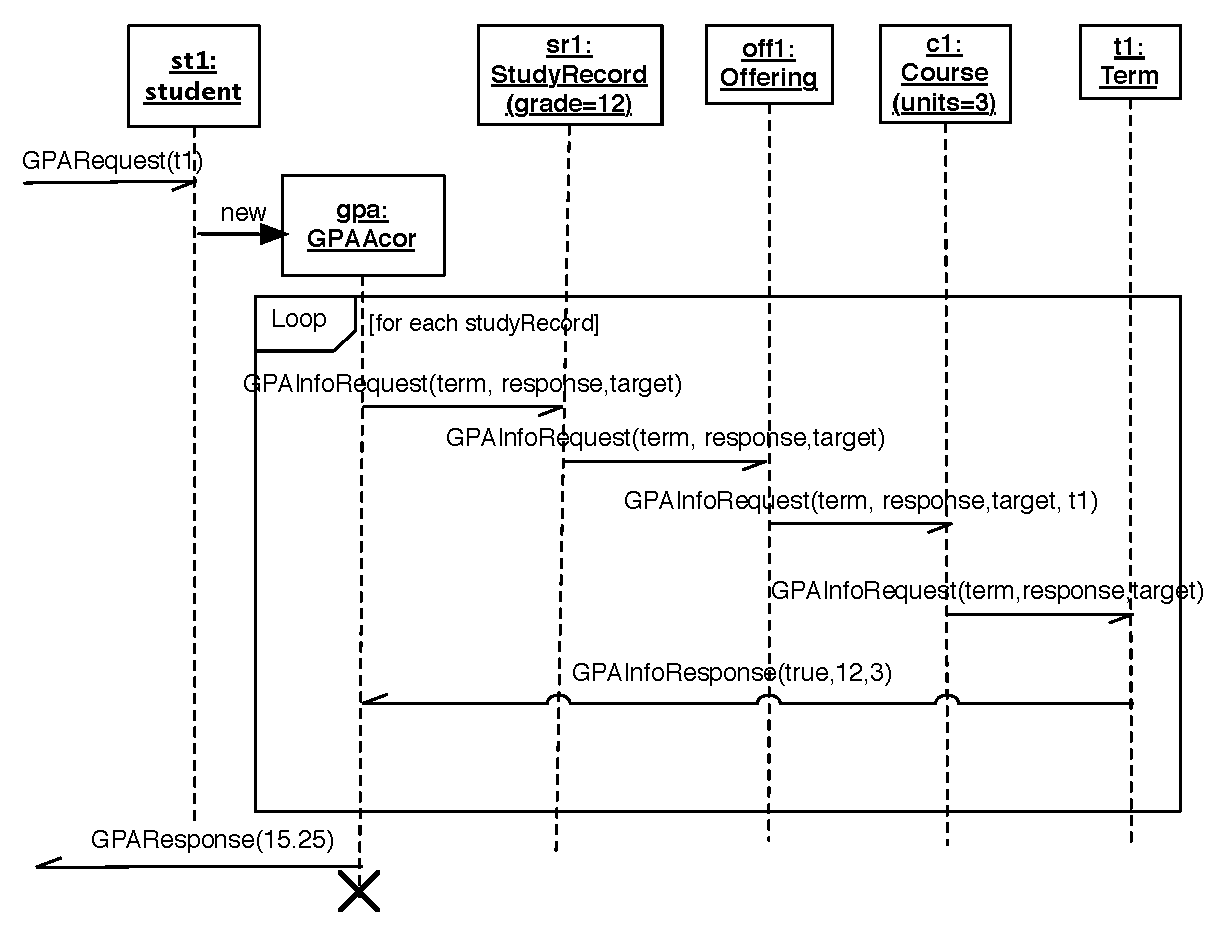
\includegraphics[width=16cm]{4-ProposedFramework/Figures/gpa_2_sequence.pdf}
    \end{center}
    \caption{\label{fig:gpa2_sequence} نمودار ترتیب برای رویکرد دوم محاسبه‌ی معدل }
\end{figure*}
\FloatBarrier
\begin{enumerate}
\item اکتور محاسبه‌ی معدل \lr{(GPAActor)}:\\
همان طور که قبلا توضیح داده شد، این اکتور برای انجام کل فعالیت‌های مربوط به یک درخواست معدل را انجام می‌دهد (در رویکرد اول این‌ کار توسط خود اکتور دانشجو انجام می‌شد).  این اکتور برای انجام وظیفه‌ی خود اولاً نیاز به برقراری ارتباط با اکتورهای سابقه دارد، و ثانیاً نیاز به دسترسی به مقصد پاسخ درخواست دارد تا بتواند نتیجه را برای آن ارسال کند. این موارد توسط اکتور دانشجو در اختیار اکتور محاسبه‌ی معدل قرار می‌گیرد. شبه کد \ref{fig:usecases:gpa:2:gpaActor} نحوه‌ی طراحی این اکتور را نشان می‌دهد. اکتور محاسبه‌ی معدل با شروع به کار پیغام‌های لازم برای سایر اکتور‌ها را ارسال می‌کند و با گرفتن هر پاسخ، متغیر‌های حالت خود را بروزرسانی می‌کند. پایان کار این اکتور زمانی مشخص می‌شود که به تعدادی که پیغام ارسال کرده پاسخ دریافت کند. این تعداد برابر با تعداد اکتورهای سابقه است. بنابراین پس از دریافت این تعداد پیغام، معدل محاسبه شده را برای مقصد نهایی ارسال می‌کند.

\codelisting[language=scala]{4-ProposedFramework/src/usecases/gpa/2/GPAActor.scala}{شبه‌کد طراحی اکتور محاسبه‌ی معدل در رویکرد ۲.}{fig:usecases:gpa:2:gpaActor} 

تغییر مهم اکتور دانشجو این است که با توجه به واگذاری عملیات محاسبه‌ی معدل به اکتوری دیگر، نیازی به نگهداری متغیرهای حالت که به این منظور ایجاد شده بودند، ندارد. شبه کد 
اکتور دانشجو در رویکرد جدید در شکل \ref{fig:usecases:gpa:2:student}  نشان داده شده است. مقایسه‌ی طراحی این اکتور در دو رویکرد نشان می‌دهد که با انجام این عمل، طراحی اکتور دانشجو بسیار ساده‌تر شده است.

\codelisting[language=scala]{4-ProposedFramework/src/usecases/gpa/2/Student.scala}{شبه‌کد طراحی اکتور دانشجو در رویکرد ۲.}{fig:usecases:gpa:2:student} 
\FloatBarrier

\end{enumerate}
%۱: نقش سابقه در این پیغام‌ها چیه؟ یکی اینکه نمره دست اونه و دیگه اینکه راهیه که به بقیه اطلاعات برسیم. اولی باعث می‌شه که حتما به دست اون برسه. ولی آیا اینکه جواب اول دست سابقه برسه بعد به دانشجو برسه الزامیه؟ با توجه به اینکه یک بار از زیر دستش رد می‌شه و دفعه‌ی دوم فقط relay می‌کنه.
%۲: یادآوری سوال ۲ بخش قبل. تاکید بر اینکه این بده چون ما همروندی رو پایین میاریم. آیا راهی برای این کار وجود نداره؟ یه اکتور درست می‌کنیم که فقط اینو ....
%۳: هیچ جا نمی‌شه مسیرو کوتاهتر کرد؟ زودتر جواب آخر رو فرستاد؟ منظور اینه که از domain بفهمیم. در این مورد اگر مربوط به ترم نباشه اصلا حساب نمی‌شه. پس اگه ترم ۱ سره بتونه جواب بده خیلی خوبه.
\subsubsection{مقایسه‌ی دو رویکرد}
در بخش‌های قبلی ۲ رویکرد متخلف برای طراحی اکتورها در ارتباط با مورد کاربرد محاسبه‌ی معدل معرفی شده و مراحل انجام طراحی در آنها شرح داده شد. علیرغم صحت عملکرد هر دو رویکرد، تفاوت‌های کیفی در طراحی به وسیله‌ی این دو رویکرد حائز اهمیت هستند. به همین دلیل در این بخش به مقایسه‌ی این دو رویکرد می‌پردازیم.\\
رویکرد دوم دو تغییر عمده نسبت به رویکرد اول دارد:
\begin{enumerate}
\item قرار دادن مقصد نهایی درخواست در داخل پیغام:\\
در رویکرد اول هر اکتوری که پیغامی را به عنوان درخواست از یک اکتور دیگر دریافت می‌کند، وظیفه‌ی پاسخ به آن را نیز به عهده دارد. در صورتی که برای پاسخ به درخواست نیاز به برقراری ارتباط با اکتورهای دیگر وجود داشته باشد،‌این اکتور اقدام به ارسال پیغام‌های مرتبط به سایر اکتورها می‌کند و در نهایت با جمع‌آوری پاسخ‌ها، درخواست اصلی را پاسخ می‌دهد. با اینکه این رویکرد از دیدگاه طراحی شیءگرا به روش ترتیبی،‌ رویکردی متداول و حتی اجباری است\footnote{در طراحی شیءگرای ترتیبی، مکانیزم کنترل برنامه فراخوانی متد است. با هر فراخوانی متد، منطق پیاده شده در متد اجرا می‌شود و پس از بازگشت از متد، اجبارا کنترل برنامه به همان قسمتی که متد فراخوانی شده بود برمی‌گردد.}، در مدل تبادل پیغام این امکان وجود دارد که پاسخ درخواست را اکتوری غیر از دریافت کننده‌ی درخواست ارسال کند. لازم به ذکر است که در مدل اکتور هیچ فرضی در مورد مشخصات فرستنده‌ی پیغام صورت نمی‌گیرد. بنابراین یک اکتور می‌تواند به جای اینکه پس از ارسال پیغام‌های مربوط به یک درخواست، منتظر دریافت جواب برای فرستادن به درخواست کننده بماند،‌ آدرس (نام) مقصد نهایی را در داخل پیغام برای اکتور ها ارسال کند تا در صورت لزوم از آن برای فرستادن نتیجه استفاده کنند. رویکرد دوم در واقع از این امتیاز استفاده کرده و به این روش از تعدادی از تبادلات پیغام که صرفاً به دلیل ذکر شده صورت می‌گیرند، جلوگیری می‌کند. با این کار نیازی به برگشت پیغام در همان مسیری که طی شده وجود نخواهد داشت و در هر لحظه که اطلاعات لازم برای تکمیل پاسخ تأمین شود، پاسخ به مقصد ارسال خواهد شد.
\item واگذار کردن پردازش‌های مربوط به یک درخواست به یک اکتور موقت:\\
 در رویکرد اول اکتور دانشجو، پس از ارسال پیغام‌های لازم و دریافت جواب، تمام محاسبات لازم برای تعیین معدل را انجام ‌می‌داد. در اثر استفاده از این رویکرد، اولاً دانشجو باید تعدادی پیغام برای تهیه‌ی اطلاعات لازم جهت محاسبه‌ی معدل به سایر اکتورها ارسال کرده و منتظر جواب بماند، ثانیاً برای محاسبه‌ی معدل اطلاعات موقتی را به عنوان متغیر حالت در خود نگهداری کند. مقدار این متغیر‌ها فقط در زمانی که یک درخواست مشخص در حال پردازش است معتبر است به همین دلیل در صورت شروع به پردازش درخواست‌های دیگر قبل از اتمام عملیات مربوط به درخواست قبلی امکان‌پذیر نمی‌باشد. در نتیجه میزان همروندی در درخواست‌های مشابه پایین می‌آید. از طرف دیگر در صورتی که قرار باشد، اکتور انواع متعددی از درخواست‌هایی را که این خاصیت را دارند پردازش کند، مدیریت پیچیدگی حاصل از اطلاعات حالت مربوط به درخواست‌های مختلف نیز کار آسانی نخواهد بود و منجر به پیچیدگی زیاد  و تغییرپذیری کمتر کلاس خواهد شد. به همین دلایل در رویکرد دوم سیاست جدید اتخاذ شد و آن سپردن کل فعالیت‌های محاسبه‌ی معدل به یک اکتور جدید است. با این کار دو نتیجه‌ی مطلوب حاصل می‌شود. اولاً پیچیدگی‌های مربوط به اجرای یک درخواست به اکتور دیگری منتقل می‌شود که صرفاً برای پاسخ به درخواست مورد نظر طراحی شده است. ثانیا با توجه به اینکه هر نمونه از اکتور جدید صرفاً محدود به یک درخواست بوده و پس از پاسخ به‌ آن به فعالیت خاتمه می‌دهد، امکان پاسخ به درخواست‌های همروند به درخواست‌ها هم به وجود می‌آید.
\end{enumerate}
لازم به ذکر است که هدف از معرفی این دو رویکرد در طراحی منطق مربوط به محاسبه‌ی معدل صرفاً تأکید بر تفاوت‌های آنها و حفظ وضوح روش طراحی دارد. طبیعتاً علیرغم صحت رویکرد اول، در ادامه‌ی طراحی از سیاست‌های ذکر شده در رویکرد دوم استفاده خواهد شد
\subsection{مورد کاربرد اخذ درس}
در بخش قبل مراحل طراحی مورد کاربرد محاسبه‌ی معدل با استفاده از دو رویکرد مختلف توضیح داده شد. در این بخش مراحل طراحی مورد کاربرد اخذ درس با توجه به تجربیات حاصل از بخش قبل ارائه می‌گردد. \\
توصیف مورد کاربرد اخذ درس در جدول \ref{table:uc_takecoure} ارائه شد. دانشجو در زمان انتخاب واحد یکی از ارائه‌\LTRfootnote{Offering}های موجود ترم را انتخاب می‌کند. سیستم شرایط لازم برای اخذ این ارائه را بررسی می‌کند. در صورتی که دانشجو مجاز به انتخاب این ارائه باشد، یک سابقه از ارائه‌ی مورد نظر را برای دانشجو ذخیره می‌کند. در صورتی که هر کدام از شرایط لازم برای اخذ محقق نشده باشد سیستم یک پیغام خطا برای کاربر نمایش می‌دهد.
همانند مورد کاربرد قبل،‌ این مورد کاربرد هم با دریافت یک پیغام توسط اکتور دانشجو آغاز می‌شود. تنها اطلاعاتی که در این پیغام باید موجود باشد ارائه‌ی انتخاب شده برای اخذ است. بنابراین فرمت پیغام درخواست اخذ درس به شکل زیر خواهد بود:
\begin{latin}
TakeCourseRequest(offering: Offering)
\end{latin}
پاسخ این درخواست نیز باید حاوی نتیجه‌ی عملیات و نیز احتمالاً یک پیغام برای کاربر خواهد بود. بنابراین پیغام پاسخ اخذ درس به فرمت زیر خواهد بود:
\begin{latin}
TakeCourseResponse(result: Boolean, comment: String)
\end{latin}
مطابق توضیحاتی که در طراحی مورد کاربرد محاسبه‌ی معدل داده ‌شد، اکتور دانشجو در مواجهه با پیغام درخواست اخذ دو راهکار کلی پیش رو دارد. راهکار اول این است که منطق مورد نیاز برای پردازش اخذ درس را خودش پیاده‌سازی کند (مانند رویکرد اول در طراحی مورد کاربرد محاسبه‌ی معدل) و راهکار دوم این است که به یک اکتور دیگر وکالت این محاسبات را بسپارد. همان‌طور که در بخش قبل ذکر شد،‌ تصمیم به سپردن محاسبات به کاربرد دیگر به دو انگیزه‌ی مختلف صورت می‌گیرد. انگیزه‌ی اول جلوگیری از پیجیده و بزرگ شدن یک اکتور در اثر پردازش پیغام‌های مختلف و انگیزه‌ی دوم ایجاد امکان همروندی در پردازش پیغام‌های مشابه.\\
در این مورد کاربرد هر دو انگیزه برای سپردن محاسبات به یک اکتور دیگر معتبر می‌باشند: اکتور دانشجو در مدل دامنه‌ی معرفی شده، مسئولیتِ دریافت اکثر درخواست‌های کاربران را به عهده دارد (به دلیل اینکه کاربر اصلی این سیستم دانشجو است)، درخواست‌های مختلفی را دریافت خواهد کرد. به همین دلیل در صورتی که  پردازش تمام این پیغام‌ها را بر عهده بگیرد، اندازه و پیچیدگی آن زیاد شده و در نتیجه تغییرپذیری آن تنزّل خواهد کرد (انگیزه‌ی اول). علاوه بر این، اکتور دانشجو برای پردازش هر درخواست اخذ درس، باید شروط مختلفی را بررسی کند و برای این کار با اکتورهای دیگر به دفعات تبادل پیغام انجام خواهد داد و برای حفظ نتایج میانی تبادلات پیغام تا پایان پردازش درخواست، مجبور به استفاده از متغیرهای حالت اکتور (فیلدهای داده‌ی محلی) خواهد بود (مشابه متغیرهایی که در محاسبه‌ی معدل استفاده شد). در نتیجه پردازش همروند درخواست‌های اخذ درس بسیار پیچیده و یا نشدنی خواهد بود. بنابراین در این مورد، ایجاد همروندی در پردازش درخواست‌ها نیز انگیزه‌ی معتبری برای سپردن محاسبات به یک اکتور دیگر است (انگیزه‌ی دوم). \\
\subsubsection{ اکتور اخذ درس}
\label{section:takeCourse}
با توجه به توضیحات ذکر شده اکتور دانشجو با گرفتن درخواست اخذ درس، کلیه‌ی محاسبات لازم و ارسال پاسخ را به اکتور اخذ درس منتقل می‌کند. وظیفه‌ی اکتور اخذ درس بررسی شرایط دانشجو برای اخذ درس و ارسال پاسخ درخواست است. طبق توصیف مورد کاربرد اخذ درس (جدول \ref{table:uc_takecoure})، شروطی که باید قبل از قبول اخذ درس بررسی شوند عبارتند از:
\begin{enumerate}
\item دانشجو در ترم‌های قبل درس مربوط به ارائه‌ی انتخاب شده را  نگذرانده باشد.
\item دانشجو در ترم‌ جاری این درس را اخذ نکرده باشد.
\item دانشجو تمام پیش‌نیاز‌های این درس را با موفقیت گذرانده باشد.
\item تعداد واحد‌های اخذ شده توسط دانشجو در این ترم پس از اخذ این درس بیشتر از ۲۰ نشود.
\end{enumerate}
در این مرحله، اکتور اخذ درس باید برای هریک از شروط ذکر شده، اولاً قالب پیغام مناسب را طراحی کند، ثانیاً مقصد پیغام را مشخص کند (تشخیص اکتور مسئول). این دو مورد باید برای هریک از چهار شرط فوق بررسی شوند. در ادامه بررسی این موارد برای شرط اول به صورت مبسوط بررسی می‌شود و برای سایر شروط با توجه به شباهت به شرط اول صرفاً نتیجه‌ی بررسی ارائه می‌گردد:
\begin{itemize}
\item شرط ۱:\\
 این شرط باید تعیین کند که دانشجو قبلاً سابقه‌ای از گذراندن این درس را دارد یا خیر. قبل از انتخاب قالب پیغام، بحثی در مورد پذیرنده‌ی پیغام (اکتور مسئول) می‌کنیم. گزینه‌های موجود برای اکتور مسئول بررسی شرط گذراندن درس باشد اینها هستند:
 \begin{enumerate}
 \item خود اکتور اخذ درس:\\
  انتخاب اول در واقع به این معنی است که اکتور اخذ درس به جای اینکه درخواستی برای بررسی گذرانده شدن درس ارسال کند،‌ خود این بررسی را به عهده بگیرد. البته این به این معنی نیست که برای انجام این بررسی هیچ پیغامی به اکتورهای دیگر ارسال نکند، بلکه به این معنی است که وظیفه‌ی پیاده‌سازی منطق لازم برای رسیدن به پاسخ این پرسش (آیا این دانشجو قبلاً این درس را گذرانده است؟) بر عهده‌ی اکتور اخذ درس باشد. این حالت به دو دلیل مناسب نیست: اولاً در این حالت اکتور اخذ درس به صورت ابتدا به ساکن (بدون دریافت درخواستی برای این کار) اقدام به پیاده‌سازی یک منطق کرده است. در نتیجه این پیاده‌سازی به جز این اکتور برای اکتور دیگری قابل استفاده‌ی مجدد نیست.
 \footnote{  البته یک راهکار ممکن برای برطرف کردن این مشکل این است که به اکتور اخذ درس، قابلیت دریافت پیغامی از نوع بررسی شرط مذکور اضافه شود و این اکتور برای بررسی این شرط، یک پیغام به خودش بفرستد تا به این صورت قابلیت استفاده‌ی مجدد داشته باشد. اما ایراد این رویکرد این است که از نظر منطقی اضافه کردن این رفتار به اکتوری که صرفاً وظیفه‌ی پاسخ به یک درخواست اخذ درس را دارد، از نظر تقسیم مسئولیت عمل درستی نیست.}
  ثانیاً با توجه به اینکه این اکتور شروط متعددی را بررسی می‌کند، پیاده کردن منطق بررسی این شروط خوانایی کلاس را کاهش می‌دهد. 
 
  البته یک راهکار ممکن برای برطرف کردن این مشکل این است که به اکتور اخذ درس، قابلیت دریافت پیغامی از نوع بررسی شرط مذکور اضافه شود و این اکتور برای بررسی این شرط، یک پیغام به خودش بفرستد تا به این صورت قابلیت استفاده‌ی مجدد داشته باشد. اما ایراد این رویکرد این است که از نظر منطقی اضافه کردن این رفتار به اکتوری که صرفاً وظیفه‌ی پاسخ به یک درخواست اخذ درس را دارد، از نظر تقسیم مسئولیت عمل درستی نیست. 
 \item اکتور جدیدی که به این منظور تولید می‌شود:\\
 این رویکرد ایرادهای شمرده شده برای انتخاب اول را ندارد. اما با فرض این که درخواست بررسی گذرانده شدن درس یک درخواست قابل استفاده‌ی مجدد در منطق دامنه‌ی سیستم باشد، با این رویکرد در هر قسمتی از برنامه که نیاز به بررسی این درخواست وجود داشته باشد، باید اکتوری به این منظور ایجاد شود و اطلاعات لازم به آن داده شود و سپس درخواست برای آن ارسال شود. از نظر طراحی شیءگرا، تکرار این عملیات در هر بار نیاز به این درخواست پدیده‌ی مطلوبی نمی‌باشد.
 \item اکتور دانشجو:\\
 انتخاب اکتور دانشجو برای ارسال درخواست بررسی گذرانده شدن درس علاوه بر اینکه ایرادهای مطرح شده در گزینه‌ی اول را ندارد، مشکل تکرار عملیات (گزینه‌ی دوم) را نیز ندارد. در این حالت، هر اکتوری که نیاز به بررسی درخواست گذرانده شدن درس را داشته باشد، پیغام مربوطه را برای اکتور دانشجو ارسال می‌کند و تنها جایی که عملیات ایجاد اکتور جدید برای پردازش این درخواست انجام می‌شود اکتور دانشجو است. از نظر منطق دامنه نیز بررسی گذرانده شدن درس توسط اکتور دانشجو انتخاب مطلوبی به نظر می‌رسد.
 \end{enumerate}
 با توجه به استدلال فوق، اکتور اخذ درس، اکتور دانشجو را به عنوان مسئول بررسی گذرانده شدن درس انتخاب می‌کند.\\
 با انتخاب مقصد پیغام درخواست بررسی گذرانده شدن درس، طراحی قالب پیغام آن به آسانی انجام می‌شود. با توجه به اینکه این پیغام به مقصد اکتور دانشجو ارسال می‌شود، تنها داده‌ای که لازم است در آن قرار داده شود درس مربوطه است. بنابراین قالب پیغام درخواست به صورت زیر می‌باشد:
 \begin{latin}
 PassedRequest(course:Course)
 \end{latin}
 پیغام پاسخ کافی‌ است که اطلاع دهد که درس مورد نظر گذرانده شده است یا خیر. بنابراین قالب پیغام پاسخ به صورت زیر می‌باشد:
 \begin{latin}
PassedResponse(result:Boolean)
 \end{latin}
% با توجه به توضیحات داده‌ شده، طراحی اکتور اخذ درس تا این مرحله از طراحی به صورت شبه‌کد شکل بلاه خواهد بود.

\item شرط ۲:\\
 این شرط باید تعیین کند که دانشجو قبلاً در همین ترم این درس را اخذ کرده است یا خیر. با استدلال مشابه شرط ۱ به این نتیجه می‌رسیم که مقصد پیغام درخواست بررسی اخذ تکراری اکتور دانشجو است و قالب پیغام‌های درخواست و پاسخ برای این شرط به صورت زیر می‌باشد:
 \begin{latin}
 TakenRequest(course:Course)
 TakenResponse(result:Boolean)
 \end{latin}

\item شرط ۳:\\
 این شرط باید تعیین کند که دانشجو تمام پیش‌نیازهای درس را با موفقیت گذرانده است یا خیر. با استدلال مشابه شرط ۱ به این نتیجه می‌رسیم که مقصد پیغام درخواست بررسی اخذ تکراری اکتور دانشجو است و قالب پیغام‌های درخواست و پاسخ برای این شرط به صورت زیر می‌باشد:
 \begin{latin}
 PassedPresRequest(course:Course)
 PassedPresResponse(result:Boolean)
 \end{latin}
 
\item شرط ۴:\\
 این شرط کنترل می‌کند که با اخذ این درس آیا تعداد واحدهای دانشجو در ترم جاری بیشتر از ۲۰ می‌شود یا خیر. گذراندن بیش از تعدادی واحد به احتمال زیاد در چنین سیستمی به جز در بررسی شرایط کاربرد دیگری ندارد (بر خلاف موردی مثل بررسی گذرانده شدن درس که در موارد متعددی می‌تواند کاربرد داشته باشد) به همین دلیل پیغام مربوط به این مورد بهتر است به جای دانشجو به اکتور دیگری که مختص این کاربرد طراحی می‌شود سپرده شود. گیرنده‌ی پیغام مربوط به این شرط اکتور تأیید تعداد واحد (UnitsValidatorActor)  خواهد بود. با توجه به این که اکتور مذکور نیاز به دسترسی به سوابق دانشجو و نیز تعداد واحد درس انتخاب شده دارد، در هنگام ایجاد این اکتور، باید فیلد‌های دانشجو و درس را در اختیار اکتور قرار دهیم. به این ترتیب، اکتور تأیید تعداد واحد به محض ایجاد می‌تواند کار خود را شروع کند و  اکتور اخذ درس نیازی به ارسال پیغام به آن ندارد. با توجه به این توضیحات پیغام‌ پاسخ برای این شرط به صورت زیر می‌باشد:
 \begin{latin}
  UnitsValidationResponse(result:Boolean)
 \end{latin}
\end{itemize}
در این مرحله باید تعیین کنیم که اکتور بررسی اخذ درس با دریافت پاسخ هر پیغام چه عملی را باید انجام دهد:\\
هر یک از پاسخ‌هایی که اکتور بررسی اخذ درس دریافت می‌کند در واقع نتیجه‌ی بررسی یکی از شروط لازم برای اخذ درس است. برای موافقت با اخذ درس توسط دانشجو، تمام شروط باید بررسی شوند. بنابراین پاسخ موافقت با اخذ درس فقط زمانی می‌تواند ارسال شود که تمام پاسخ‌ها دریافت شوند. برای اینکه اکتور اخذ درس از اتمام دریافت دروس مطلع شود لازم است که متغیری به منظور نگه‌داری تعداد پاسخ‌هایی که باید دریافت شود ایجاد شده بروزرسانی شود. با این کار اکتور اخذ درس می‌داند که چه زمانی کار به اتمام رسیده است. اما در این مورد کاربرد، در همه‌ی حالت‌ها لازم نیست اکتور منتظر تمام پاسخ‌ها بماند. دلیل این امر این است که در صورتی که هر یک از شروط اخذ درس نقض شود، نیازی به بررسی سایر شروط نیست. مثلاً اگر دانشجو قبلاً درس را گذرانده باشد نیازی به دریافت سایر پاسخ‌ها وجود ندارد و می‌توانیم پاسخ درخواست را ارسال کنیم (خطای گذرانده شدن درس). بنابراین در این مورد کاربرد با گرفتن هر پاسخ به این ترتیب عمل می‌کنیم که اگر شرط برقرار باشد، مقدار متغیر تعداد پاسخ‌های دریافت شده را یکی زیاد می‌کنیم، اگر مقدار جدید برابر با تعداد پاسخ مورد انتظار بود (این یعنی تمام پاسخ‌ها دریافت شده‌اند)، پاسخ نهایی درخواست را ارسال می‌کنیم. و اگر شرط نقض شده باشد پاسخ درخواست را که عدم موفقیت اخذ به دلیل نقض شرایط است ارسال می‌کنیم.
نمودار شکل \ref{fig:take_course_sequence_1} تصمیمات اتخاذ شده تا این مرحله از طراحی را به صورت شماتیک نشان می‌دهد. در این نمودار حالتی بررسی شده که تمام شرایط اخذ درس برقرار شده و اخذ با موفقیت انجام می‌شود. حالت دیگری که یکی از شروط (تعداد واحد) برقرار نشده است در شکل \ref{fig:take_course_sequence_2} نشان داده شده است. در این حالت با توجه به اینکه یکی از پاسخ‌ها نشان‌دهنده‌ی این است که یکی از شروط برقرار نشده،‌ به محض دریافت این پیغام، اکتور اخذ درس نتیجه‌ی درخواست را ارسال می‌کند و به کار خود پایان می‌دهد. طبیعتا پیغام‌های دیگری که برای این اکتور ارسال شده‌اند پردازش نخواهند شد.
لازم به تأکید است که در هر دو شکل ترتیب پیغام‌ها فقط نشان دهنده‌ی یک حالت فرضی هستند. در عمل در هر بار اجرای برنامه، ترتیب گرفتن پاسخ‌ها ممکن است عوض شود.

\begin{figure*}
    \begin{center}
	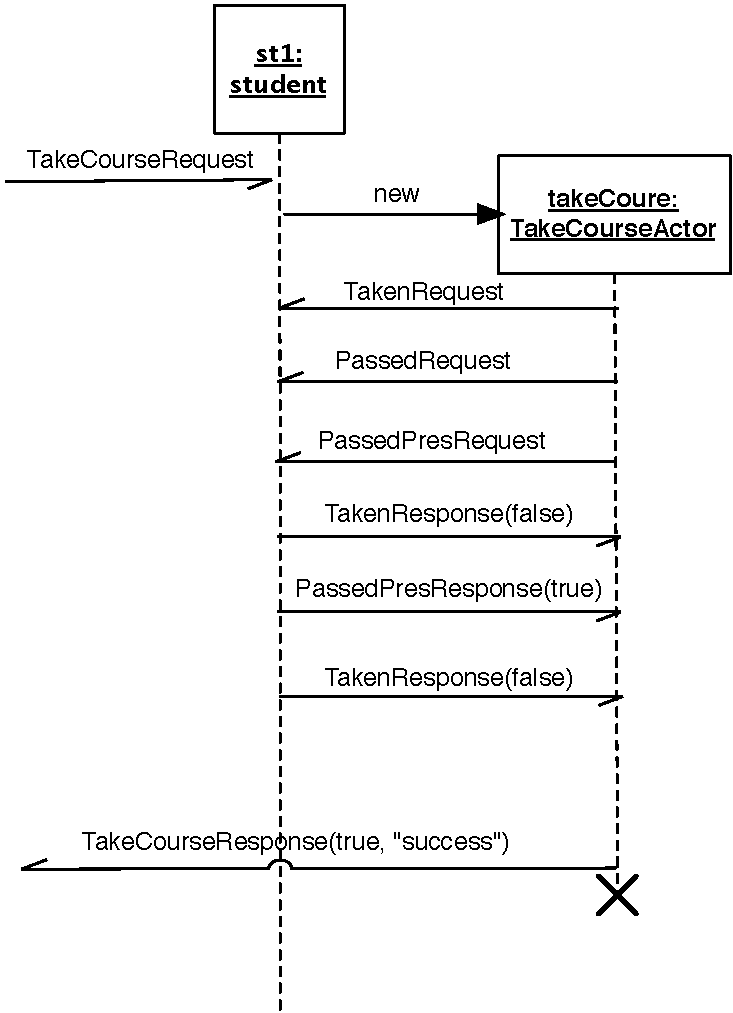
\includegraphics[width=14cm]{4-ProposedFramework/Figures/take_course_seq1.pdf}
    \end{center}
    \caption{\label{fig:take_course_sequence_1} نمودار ترتیب تبادل پیغام‌ برای اخذ درس- حالتی که تمام شروط برای اخذ برقرار است }
\end{figure*}
%\FloatBarrier

\begin{figure*}
    \begin{center}
	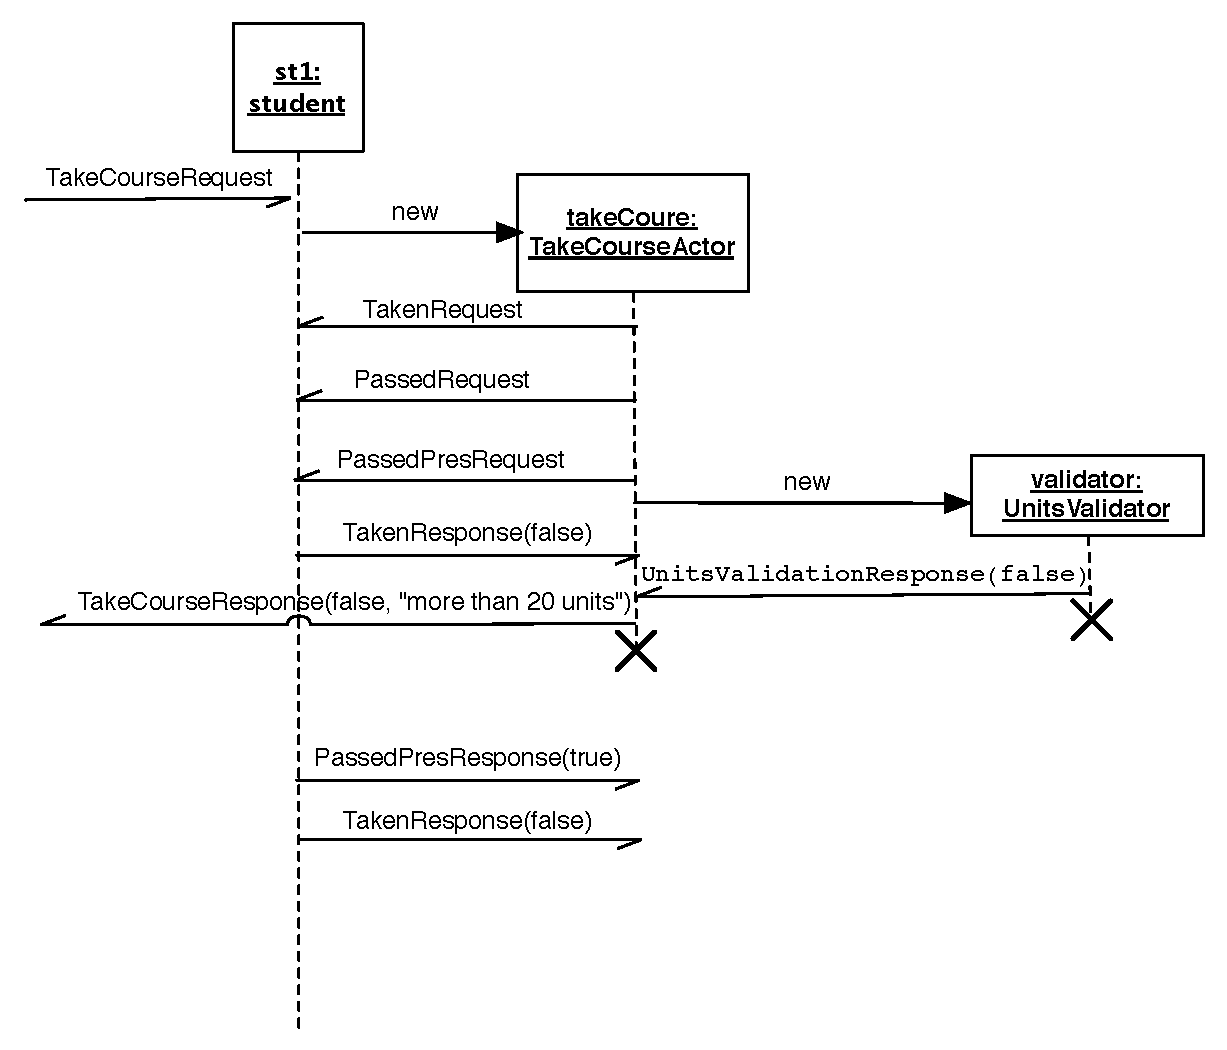
\includegraphics[width=14cm]{4-ProposedFramework/Figures/take_course_seq2.pdf}
    \end{center}
    \caption{\label{fig:take_course_sequence_2} نمودار ترتیب تبادل پیغام‌ برای اخذ درس- حالتی که یکی از شروط برقرار نیست }
\end{figure*}
%\FloatBarrier


 در این مرحله، طراحی اکتور اخذ درس به پایان رسیده است. شبه‌کد \ref{fig:usecases:take_course:take_course} ساختار کلاس اکتور اخذ درس را نشان می‌دهد.
 \codelisting[language=scala]{4-ProposedFramework/src/usecases/take_course/TakeCourseActor.scala}{شبه‌کد طراحی اکتور اخذ دانشجو.}{fig:usecases:take_course:take_course} 
%\FloatBarrier
  در ادامه باید تغییرات سایر اکتورها در اثر دریافت پیغام‌های ارسال شده از اکتور اخذ درس اعمال شود و نیز اکتور جدیدی که ایجاد شده (اکتور تایید تعداد واحد) نیز طراحی گردد.
%   برای رعایت اختصار و اجتناب از طرح نکات تکراری، جزئیات طراحی بررسی شرط گذرانده شدن درس‌ ارائه می‌گردد.
\subsubsection{بررسی گذرانده شدن درس}
\label{subsection:passCourse}
  برای بررسی گذرانده شدن درس، اکتور اخذ درس یک پیغام CoursePassRequest به اکتور دانشجو ارسال می‌کند. اکتور دانشجو بررسی این شرط را به اکتور جدید گذراندن درس\LTRfootnote{CoursePassActor} می‌سپارد. این اکتور برای بررسی گذرانده شدن درس، نیاز به برقراری ارتباط با اکتورهای سابقه\LTRfootnote{StudyRecord} دارد. بنابراین اکتور دانشجو لیست سابقه‌ی دانشجو و نیز درسی که باید گذرانده شدن آن بررسی شود را در اختیار اکتور بررسی گذراندن درس قرار می‌دهد. اکتور گذراندن درس از تمام اکتورهای سابقه سؤال می‌کند که آیا سابقه‌ی مربوطه یک گذراندن موفق از درس مذکور است یا خیر. این کار با ارسال یک پیغام با قالب زیر صورت می‌پذیرد:
  \begin{latin}
  AreYouPassCourseRequest(course)
  \end{latin}
هر اکتور سابقه‌ با دریافت این پیغام باید اولاً بررسی کند که آیا سابقه‌ای مربوط به درس مذکور است یا خیر، و ثانیاً نمره‌ی سابقه نمره‌ی قبولی است یا خیر. در اینجا با توجه به اینکه نمره‌ی مربوطه در اختیار خود اکتور سابقه است، بررسی آن ساده‌تر است. در صورتی که نمره کمتر از ۱۰ باشد، این اکتور بلافاصله پاسخ پیغام (منفی) را می‌دهد، در غیر این صورت برای بررسی این که این سابقه مربوط به درس مذکور است یا خیر، یک پیغام برای اکتور ارائه ارسال می‌کند. اکتور ارائه با گرفتن این پیغام آن را برای اکتور درس ارسال می‌کند تا این اکتور بررسی کند که آیا با درسی که در قالب پیغام دریافت کرده برابر است یا خیر. این اکتور پاسخ نهایی را مستقیماً برای اکتور بررسی گذرانده شدن درس ارسال می‌کند.  
\begin{figure}
    \begin{center}
	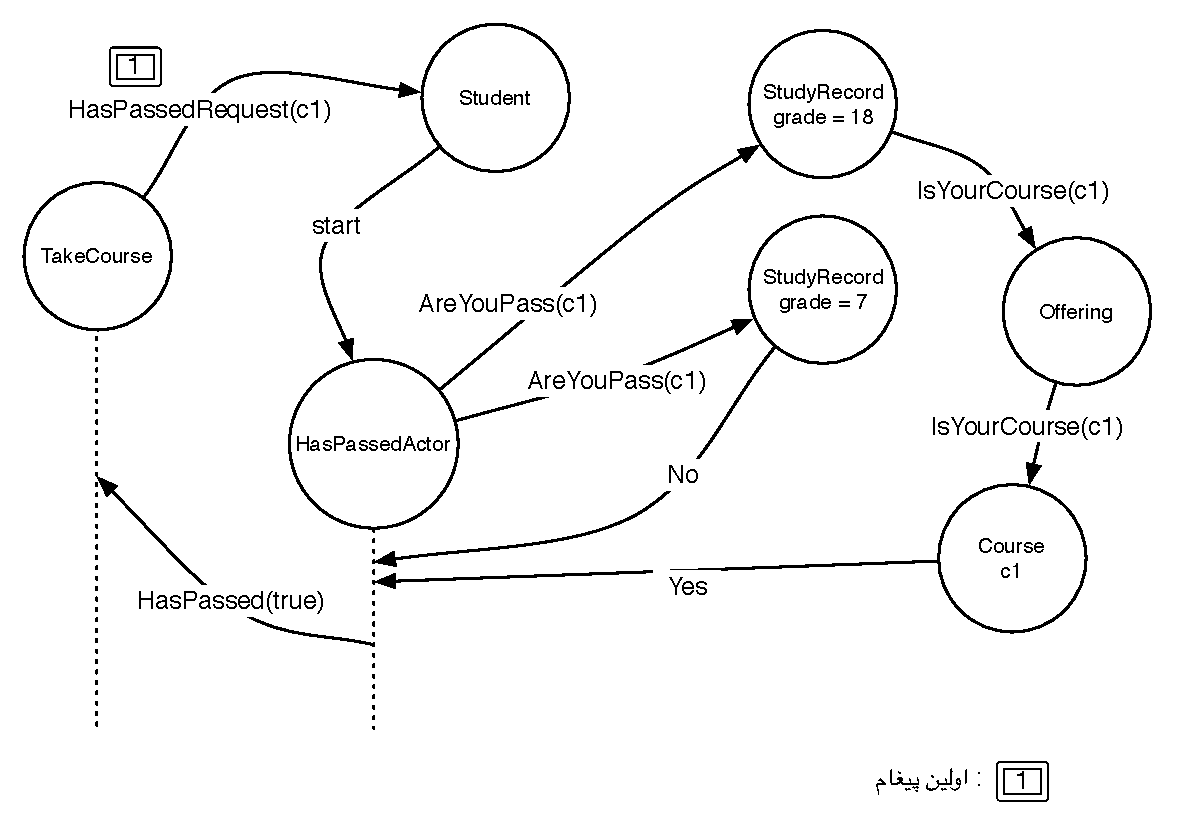
\includegraphics[width=14cm]{4-ProposedFramework/Figures/HasPassed.pdf}
    \end{center}
    \caption{\label{fig:take_course_haspassed}نمایش شماتیک تبادل پیغام بین اکتورهای مختلف برای بررسی گذرانده شدن یک درس }
\end{figure}

شکل \ref{fig:take_course_haspassed} تبادل پیغام‌های مربوط به بررسی گذرانده شدن درس را به صورت شماتیک نشان می‌دهد. در این شکل خط عمودی در حالتی به کار رفته‌ است که یک اکتور در زمان‌های مختلف پیغام دریافت کرده باشد. در مثال بررسی شده در شکل، اکتور اخذ درس یک درخواست بررسی گذرانده شدن درس (درس c1 ( را برای اکتور دانشجو ارسال می‌کند. اکتور دانشجو یک اکتور بررسی گذرانده شدن درس (HasPassedActor) ایجاد می‌کند و کار بررسی را به آن واگذار می‌کند. این اکتور پیغام‌های مناسب را برای دو اکتور سابقه‌ی دانشجو ارسال می‌کند. یکی از اکتورهای سابقه به این دلیل که نمره‌ی کمتر از ۱۰ (۷) دارد، بلافاصله پاسخ را برای اکتور مقصد ارسال می‌کند. اکتور سابقه‌ی دیگر با توجه به اینکه نمره‌ی قبولی دارد،‌ برای اطمینان از اینکه مربوط به همان درسی است که گذرانده شدن آن بررسی می‌شود، یک پیغام به اکتور ارائه ارسال می‌کند. اکتور ارائه پیغام را به درس منتقل می‌کند و اکتور درس با مقایسه‌ی درس موجود در پیغام با خودش، جواب را برای مقصد می‌فرستد.
\FloatBarrier
\subsubsection{بررسی گذرانده شدن پیش‌نیازهای درس}
اکتور دانشجو با دریافت پیغام بررسی گذرانده شدن پیش‌نیازهای درس، محاسبات مربوطه را به اکتوری که به این منظور طراحی شده ارسال می‌کند. با توجه به اینکه پیش‌نیازهای هر درس نیز خود از نوع درس هستند، در طراحی این بخش می‌توان از اکتور بررسی گذرانده شدن درس استفاده کرد. بنابراین اکتور مذکور به ازای هر کدام از پیش‌نیازهای درس، یک پیغام بررسی گذرانده شدن درس به دانشجو ارسال می‌کند. با دریافت هر پاسخ اگر مشخص شود که درسی از میان پیش‌نیازها گذرانده نشده است، بلافاصله پاسخ درخواست به مقصد (اکتور اخذ درس) ارسال می‌شود. در غیر این صورت پس از گرفتن تمام پاسخ‌ها، یک پیغام به اکتور اخذ درس ارسال می‌کند و به وسیله‌ی آن اعلام می‌کند که تمام پیش‌نیازها گذرانده شده است.
\begin{figure}
    \begin{center}
	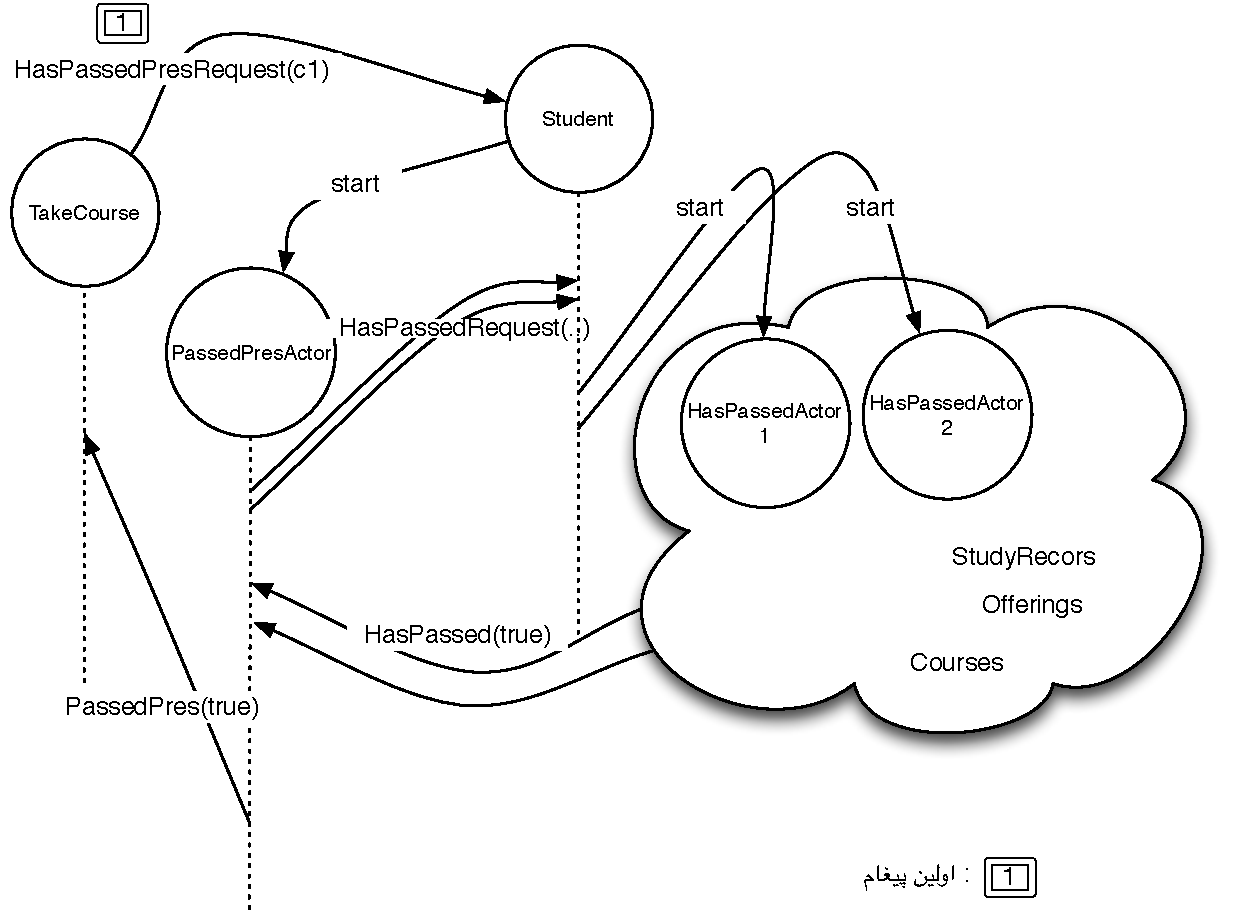
\includegraphics[width=14cm]{4-ProposedFramework/Figures/Prerequisites.pdf}
    \end{center}
    \caption{\label{fig:take_course_pres}نمایش شماتیک تبادل پیغام بین اکتورهای مختلف برای بررسی گذرانده شدن پیشنیازها‌ی یک درس }
\end{figure}
شکل \ref{fig:take_course_pres} ارتباط اکتورها برای بررسی گذرانده شدن درس نشان می‌دهد. در این شکل، ابتدا اکتور اخذ درس پیغام بررسی گذرانده شدن درس c1 را به اکتور دانشجو ارسال می‌کند. اکتور دانشجو بررسی بررسی این مورد را به اکتور بررسی پیش‌نیاز\LTRfootnote{PassPresActor} واگذار می‌کند. این اکتور به ازای هر کدام از پیشنیاز‌های  درس، یک پیغام بررسی گذرانده شدن درس برای خود دانشجو ارسال می‌کند. طراحی مورد بررسی گذراندن درس در بخش \ref{subsection:passCourse} توضیح داده شد. در این شکل برای جلوگیری از پیچیدگی طراحی، از نمایش نحوه‌ی بررسی گذرانده شدن درس صرف نظر شده است و اکتورها و پیغام‌های مربوط به آن به صورت شکل ابر نمایش داده شده است.

\FloatBarrier
\subsubsection{بررسی عدم اخذ مجدد درس}
همان‌طور که در بخش \ref{section:takeCourse} توضیح داده شد، اکتور اخذ درس یک پیغام برای بررسی عدم اخذ مجدد درس برای اکتور دانشجو ارسال می‌کند. اکتور دانشجو مطابق حالت‌های قبل بررسی این مورد را به اکتور بررسی اخذ درس\LTRfootnote{CourseTakenCheckActor} واگذار می‌کند. بررسی  اخذ شدن درس کاملاً مشابه بررسی گذرانده شدن درس است. در بررسی گذرانده شدن درس، اکتور سابقه نمره را بررسی می‌کند، در صورتی که نمره قبولی نباشد جواب را ارسال می‌کند و در صورتی که نمره قبولی باشد برای بررسی اینکه درس مربوط به سابقه همان درس مورد سؤال است یا خیر، با اکتور ارائه تبادل پیغام انجام می‌دهد. در بررسی عدم اخذ مجدد درس، از هر اکتور سابقه سؤال می‌شود که آیا سابقه مربوط به ترم جاری است یا خیر. برای اینکه  یک سابقه مربوط به ترم جاری باشد، کافی است نمره‌ای برای آن اعلام ثبت نشده باشد. بنابراین اکتور سابقه بررسی می‌کند که نمره‌ای برایش ثبت شده یا خیر اگر مقدار فیلد نمره null باشد یعنی مربوط به ترم جاری است و برای بررسی اینکه مربوط به همان درس مورد سؤال است مانند حالت بررسی گذرانده شدن درس، یک پیغام به ارائه ارسال می‌کند. در غیر این صورت حتماً جواب منفی است و بلافاصله یک پیغام برای اکتور بررسی عدم اخذ مجدد ارسال می‌شود. شکل  \ref{fig:take_course_taken} تبادل پیغام بین اکتورها برای بررسی این شرط را نشان می‌دهد. همان‌طور که مشاهده می‌شود این شکل بسیار شبیه به شکل \ref{fig:take_course_haspassed} است که بررسی گذرانده شدن درس را نشان می‌دهد.

\begin{figure}
    \begin{center}
	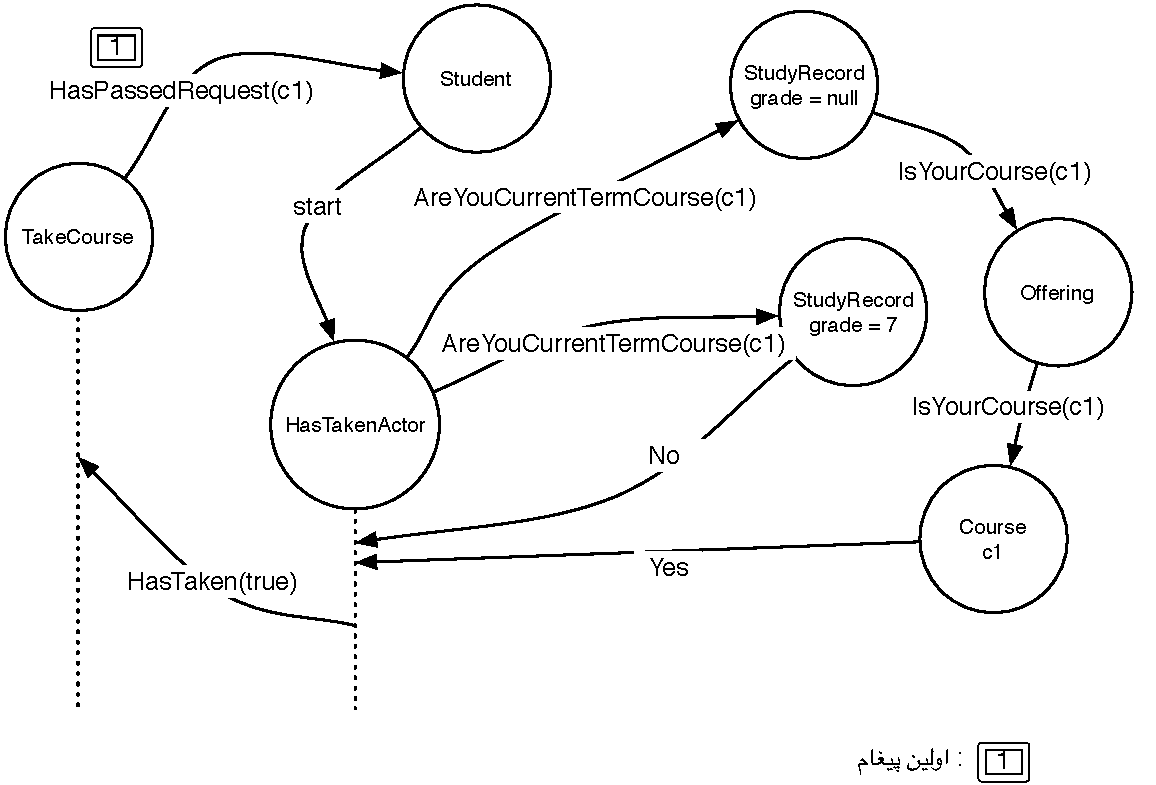
\includegraphics[width=14cm]{4-ProposedFramework/Figures/HasTaken.pdf}
    \end{center}
    \caption{\label{fig:take_course_taken}نمایش شماتیک تبادل پیغام بین اکتورهای مختلف برای بررسی عدم اخذ مجدد درس }
\end{figure}





\FloatBarrier
\subsubsection{بررسی عدم اخذ بیش از ۲۰ واحد}
در بخش طراحی اکتور اخذ درس (بخش \ref{section:takeCourse}) دیدیم که اکتور اخذ درس برای بررسی این شرط که تعداد واحدهای اخذ شده بیشتر از ۲۰ نشود، یک اکتور به این منظور ایجاد می‌کند. این اکتور با بررسی این شرط نتیجه را به صورت پیغام UnitsValidationResponse برای اکتور اخذ درس ارسال می‌کند. طراحی این کارکرد به این صورت است که اکتور مورد نظر از تمام سابقه‌های ترم درخواست می‌کند تا در صورتی که مربوط به ترم جاری هستند، تعداد واحدهای درس مربوط به خود را ارسال کنند. همان‌طور که در بخش قبل توضیح داده شد، اینکه سابقه مربوط به ترم جاری است از null بودن فیلد نمره مشخص می‌شود. بنابراین اگر فیلد نمره null نباشد اکتور سابقه عدد صفر را به عنوان تعداد واحد ارسال می‌کند. در غیر این صورت مشابه‌ حالت‌های قبل یک پیغام برای اکتور درس (از طریق اکتور ارائه) ارسال می‌کند تا تعداد واحدها را به اکتور مقصد (اکتور بررسی عدم اخذ بیش از ۲۰ واحد) ارسال کند. اکتور مذکور با گرفتن هر پیغام تعداد واحدها را بروزرسانی می‌کند و با اتمام پیغام‌ها بررسی می‌کند که آیا جمع واحدها بیش از ۲۰ است یا خیر. در نهایت پاسخ را برای اکتور اخذ درس ارسال می‌کند. شکل \ref{fig:take_course_units} همکاری اکتورها برای بررسی این  شرط را به صورت شماتیک نشان می‌دهد.

\begin{figure*}
    \begin{center}
	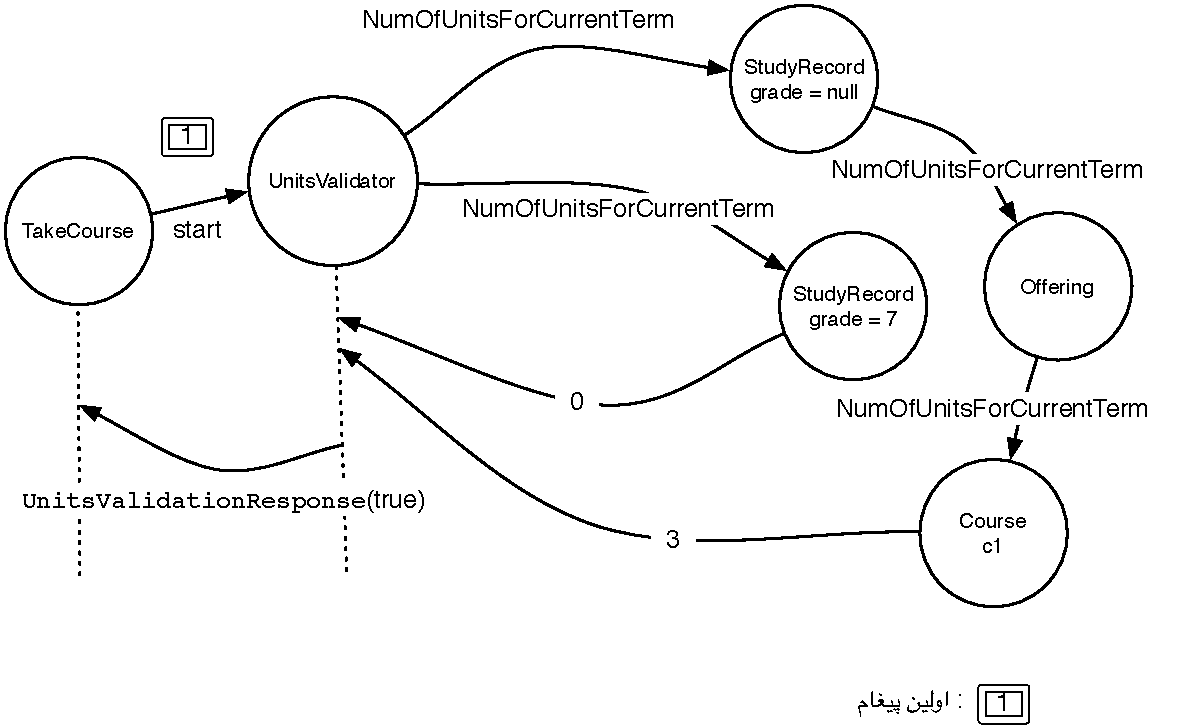
\includegraphics[width=14cm]{4-ProposedFramework/Figures/NumOfUnits.pdf}
    \end{center}
    \caption{\label{fig:take_course_units}نمایش شماتیک تبادل پیغام بین اکتورهای مختلف برای بررسی عدم اخذ بیش از ۲۰ واحد}
\end{figure*}



\section{جمع‌بندی روش و نکات مهم}
%TODO fix references to chapters
در بخش‌های پیشین  یک سیستم نمونه معرفی شد و پس از توصیف موارد کاربرد آن، روش طراحی آن با استفاده از مدل تبادل ناهمگام پیغام بررسی شد. در ادامه‌ی این فصل تلاش می‌شود با توجه به تجربیات حاصل از انجام این طراحی، روش معرفی شده به صورت نظام‌مند معرفی شود. در قسمت اول از این بخش، قدم‌های لازم برای طراحی یک سیستم به روش تبادل ناهمگام پیغام ذکر شده و در موارد ممکن، از قسمت‌هایی از سیستم طراحی شده به عنوان نمونه بهره گرفته شده است. در قسمت بعد تلاش شده الگوهای کلی هماهنگی اکتورها با تمرکز بر خواص منطق دامنه بررسی شود. در بخش بعد قسمتی از تجربیات حاصل از بررسی رویکردهای متعدد برای طراحی سیستم نمونه (سیستم آموزش ساده) ارائه شده است. و نهایتا در بخش پایانی قسمتی بحث مختصری در مورد نکات برنامه‌نویسی در هنگام پیاده‌سازی سیستم مطرح شده است.


%\subsection{ارتباط طراحی شیءگرا و طراحی به روش تبادل ناهمگام پیغام}

\subsection{گام‌های طراحی به روش تبادل ناهمگام پیغام }
روش بررسی شده در این پژوهش ارتباط تنگاتنگی با مبحث طراحی شیءگرا دارد. طراحی شیءگرا با استفاده از لفافه‌بندی\LTRfootnote{encapsulation} اشیاء منجر به تفکیک واسط کارکردی یک شیء از حالت محلی آن می‌شود و جزئیات پیاده‌سازی رفتار را مخفی ‌می‌کند. این خاصیت منجر به افزایش امکان استدلال در مورد نحوه‌ی طراحی اشیاء می‌شود. در این روش، مکانیزم کنترل اجرای برنامه‌ها فراخوانی متد است. روش تبادل ناهمگام به تفکیک کنترل اجرای منطق برنامه از زمان اجرای آن می‌پردازد. به این ترتیب قابلیت افزودن همروندی در طراحی را اضافه می‌کند. آلن کِی در \cite{Kay_messaging} اظهار داشته است که ایده‌ی اصلی در طراحی شیءگرا، ارسال پیغام بوده است. و این مسئله ارتباط تنگاتنگ طراحی شیءگرا و طراحی مبتنی بر تبادل ناهمگام پیغام را نشان می‌دهد.\\
بنابراین بسیاری از ایده‌های طراحی و تحلیل شیءگرا عیناً در این روش نیز کاربرد دارند. به همین دلیل در ارائه‌ی روش طراحی به بررسی جزئیات مواردی که دقیقاً مشابه طراحی شیءگرا هستند پرداخته نشده است. علاوه بر این، در ارائه‌ی روش فرض شده که خروجی‌های تحلیل سیستم موجود هستند. طبیعتاً روش‌های تحلیل شیءگرا و کسب شناخت از سیستم تحت طراحی، عیناً قابل اعمال در این نوع طراحی هستند. در گام‌های ذکر شده برای طراحی به روش تبادل ناهمگام، بعضی از گامها مربوط به خروجی‌های تحلیل سیستم هستند که برای حفظ انسجام، توضیح داده شده‌اند. با توجه به این موارد، در این بخش گام‌های طراحی به روش تبادل پیغام را ارائه می‌کنیم:
\begin{enumerate}
\item\textbf{شناخت سیستم و تشخیص اکتورهای دامنه}\\
شناخت سیستمی که باید طراحی شود پیش از شروع به طراحی لازم است. فعالیت‌های مربوط به این بخش مشابه همین فعالیت‌ها در روش‌های تحلیل نیازمندی‌ها و کسب شناخت\LTRfootnote{Inception} در متدولوژی‌های طراحی شیءگرا است و جزئیات آنها در حوزه‌ی این پژوهش نمی‌باشد. تعدادی از خروجی‌های این فعالیت‌ها از جمله توصیف موارد کاربرد سیستم و استخراج اشیاء دامنه به طور گسترده در طراحی مورد استفاده قرار می‌گیرند.
در مدل اکتور، همه‌ی موجودیت‌های سیستم اکتور هستند. بنابراین تمام اشیاء مدل دامنه‌ی سیستم که در مراحل ابتدایی طراحی و تحلیل شناسایی می‌شوند، به صورت اکتور طراحی می‌شوند. در منابع تحلیل و طراحی شیءگرا، روش‌هایی برای تشخیص اشیاء دامنه و نمایش مناسب آنها بیان شده است که طبیعتاً قابل اعمال در این روش نیز می‌باشند\cite{Larman_2004}. در سیستم آموزش معرفی شده، مدل دامنه در قالب نمودار کلاس در بخش \ref{subsec:mainEntities} نمایش داده شده است.
\item\textbf{انتخاب مورد کاربرد برای طراحی جزئیات}\\
با در دست داشتن موارد کاربرد و اشیاء دامنه، فعالیت‌های مربوط به طراحی اکتورهای سیستم آغاز می‌گردد. در گام اول نیاز داریم یکی از موارد کاربرد را برای طراحی انتخاب کنیم. معمولاً انتخاب مورد کاربرد با توجه به اولویت و اهمیت‌ آن صورت می‌پذیرد. پس از انتخاب مورد کابرد باید رخداد‌های سیستمی آن شناسایی شوند. این رخدادها نتیجه‌ی تعامل بازیگران خارجی با سیستم هستند. استخراج رخداد‌های سیستمی با توجه به موارد کاربرد صورت می‌گیرد. این رخدادها را می‌توان با استفاده از نمودارهای ترتیب سیستمی\LTRfootnote{system sequence diagram (SSD)} نمایش داد\cite{Larman_2004}. در نمودار ترتیب سیستمی، سیستم به صورت جعبه‌ی سیاه\LTRfootnote{black box} درنظر گرفته می‌شود و تعامل بازیگر خارجی با سیستم به صورت فرستادن درخواست و دریافت پاسخ نمایش داده می‌شود. 
به عنوان مثال شکل \ref{fig:ssd} نمودار ترتیب سیستمی را برای سناریوی اصلی مورد کاربرد محاسبه‌ی معدل نشان می‌دهد. رخدادهای سیستمی نقطه‌ی مناسبی برای شروع به طراحی اکتورها و ارتباطات آنها هستند. در طراحی شیءگرای ترتیبی، رخدادهای سیستمی در ارتباطی تنگاتنگ با متدهای یک شیء قرار دارند. در واقع نقطه‌ی آغاز اجرای محاسبات مربوط به یک رخداد سیستمی یک متد است. دلیل این پیش‌فرض این است که مکانیزم کنترل برنامه در طراح شیءگرای ترتیبی (و هر روش ترتیبی دیگر) فراخوانی متد است. در حالی که در روش مبتنی بر اکتور، مکانیزم ارتباطی تبادل پیغام است. بنابراین در این روش هر رخداد سیسستمی به یک پیغام نگاشت می‌شود که به دست یکی از اکتورها سیستم می‌رسد. 
\begin{figure*}[bh]
    \begin{center}
	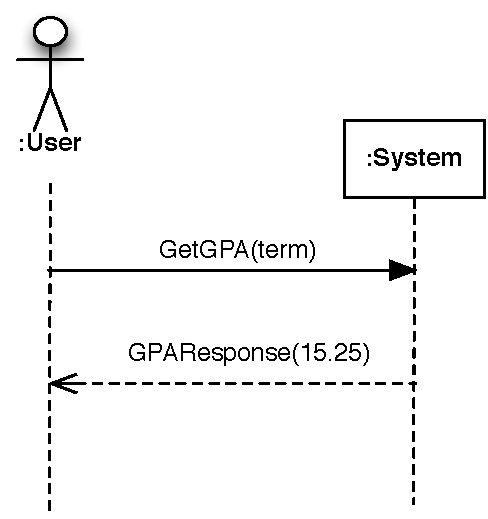
\includegraphics[width=6cm]{4-ProposedFramework/Figures/ssd.pdf}
    \end{center}
    \caption{\label{fig:ssd}نمودار ترتیب سیستمی برای یک سناریو از مورد کاربرد محاسبه‌ی معدل}
\end{figure*}

\item\textbf{انتخاب اکتور مسئول برای دریافت اولین پیغام}\\
همان‌طور که در مورد قبل توضیح داده شد، در مدل طراحی اکتور، وقوع یک رخداد سیستمی، به وسیله‌ی ارسال پیغام صورت می‌گیرد. گام اول در طراحی سیستم به هدف پاسخگویی به این پیغام این است که مشخص شود کدام اکتور باید اولین پیغام را دریافت کند. این مورد در طراحی شیءگرا در قالب مفهوم \textbf{مسئولیت شیء} بیان می‌شود. در طراحی شیءگرا شیءای موظف به دریافت درخواست است که مسئولیت درخواست با آن باشد. تشخیص مسئولیت با توجه به منطق دامنه صورت می‌گیرد و بدون در نظر گرفتن منطق دامنه، قاعده‌ای برای انتخاب شیء مسئول وجود ندارد. مسئولیت اشیاء از نظر نوع به دو دسته‌ی کلی مسئولیت \textit{انجام}\LTRfootnote{Doing Responsibilities} (مانند مسئولیت ایجاد یک شیء و آغاز یک عملیات) و مسئولیت \textit{اطلاع}\LTRfootnote{Knowin Responsibilities} (مانند اطلاع از اشیاء مرتبط یا اطلاع از داده‌های محلی لفافه‌بندی شده) تقسیم می‌شود\cite{Larman_2004,rdd}.
معمولاً  مسئولیت پاسخگویی به درخواست‌های سیستمی بعد از  تهیه‌ی مدل دامنه آسان‌تر می‌شود. در سیستم بررسی شده در این پژوهش مسئولیت پاسخ‌گویی به درخواست محاسبه‌ی 
معدل اکتور دانشجو است. با مشخص شدن اکتور مسئول برای دریافت پیغام، در ادامه‌ی طراحی باید روش پردازش پیغام در اکتور مورد نظر بررسی گردد.
\item\textbf{منطق پردازش درخواست}\\
تا این مرحله از طراحی، مشخص شده است که اکتور مسئول برای دریافت پیغام درخواست کدام است. در این مرحله باید تصمیم گرفته شود که نحوه‌ی پردازش پیغام درخواست به چه صورتی خواهد بود. پردازش پیغام به دو صورت کلی انجام می‌پذیرد. حالت اول این است که خود اکتور مسئولیت پردازش پیغام را بر عهده بگیرد. در این حالت اکتور مذکور یا به تنهایی قادر به انجام تمام عملیات مرتبط با درخواست دریافت شده است و یا با همکاری اکتورهای دیگر می‌تواند منطق مربوط به درخواست را اجرا کند. 

حالت دوم  به این صورت است که اکتور تصمیم بگیرد که اکتور جدیدی را به منظور پردازش این درخواست ایجاد کند و تمام عملیات مربوط به درخواست را به این اکتور واگذار کند. حالت مشابه‌ این مورد در طراحی شیءگرای ترتیبی نیز رخ می‌دهد. در طراحی شیءگرا ممکن است به دلیل جلوگیری از افزایش پیچیدگی کلاس و  حفظ قابلیت تغییر، تمام کار پردازش یک درخواست را به کلاس دیگری که به همین منظور ایجاد می‌شود منتقل کند. در روش طراحی مبتنی بر تبادل ناهمگام، علاوه بر این مورد به دلیل دیگری نیز این تصمیم اتخاذ می‌شود. این مسئله در ادامه در قالب یک مثال توضیح داده می‌شود:\\
فرض کنید یک مدل دامنه از ۳ اکتور تشکیل شده باشد. اکتور A که یک متغیر محلی عددی به نام a دارد. این اکتور یک نوع پیغام دریافت می‌کند: پیغام getA که در پاسخ آن مقدار a را ارسال می‌کند. اکتور B به طور مشابه یک متغیر محلی عددی به نام b دارد و با دریافت پیغام getB مقدار b را ارسال می‌کند. اکتور سوم Sum نام دارد که با دریافت پیغام sum باید مجموع مقادیر a و b را ارسال کند. اکتور Sum چون از مجموع a و b اطلاع ندارد برای پاسخ به پیغام sum نیاز به همکاری A و B دارد. فرض کنیم اکتور Sum به این شکل طراحی می‌شود که با دریافت پیغام sum ابتدا متغیرهای محلی s و count را صفر می‌کند و سپس پیغام‌های getA و getB را برای اکتورهای A و B ارسال می‌کند با دریافت هر پاسخ مقدار count را یکی زیاد می‌کند و متغیر s را با عدد دریافت شده جمع می‌کند. بعد از دریافت هر پاسخ و بروزرسانی متغیرهای داخلی، اگر مقدار count برابر با عدد ۲ شد (یعنی هر دو پاسخ دریافت شده است) مقدار متغیر s (حاصل‌جمع) را به عنوان پاسخ درخواست ارسال می‌کند. شکل \ref{fig:coord1} همکای این ۳ اکتور برای پاسخ به درخواست sum را نشان می‌دهد.
\begin{figure*}[h]
    \begin{center}
	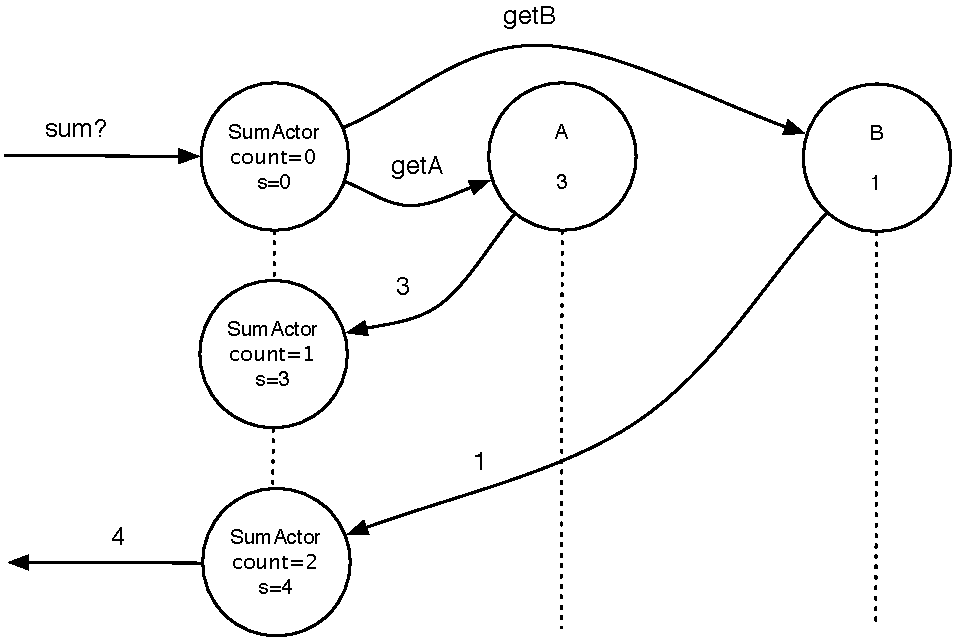
\includegraphics[width=10cm]{4-ProposedFramework/Figures/ExampleCoord1.pdf}
    \end{center}
    \caption{\label{fig:coord1} همکاری موفق اکتورها برای پاسخ به درخواست مجموع a و b}
\end{figure*}
مشکل این طراحی زمانی مشخص می‌شود که اکتور Sum بعد از دریافت پاسخ‌ A و قبل از دریافت پاسخ B یک درخواست sum دیگر دریافت می‌کند. اکتور Sum برای پاسخ به این درخواست مقدار متغیرهای s و count را صفر می‌کند و دو پیغام جدید برای A و B ارسال می‌کند. در این هنگام اکتور Sum پاسخ B برای درخواست اول را دریافت می‌کند اما چون مقدار متغیر count صفر است، متوجه اتمام عملیات درخواست اول نمی‌شود. شکل \ref{fig:coord2} این حالت را نمایش می‌دهد.
\begin{figure*}[h]
    \begin{center}
	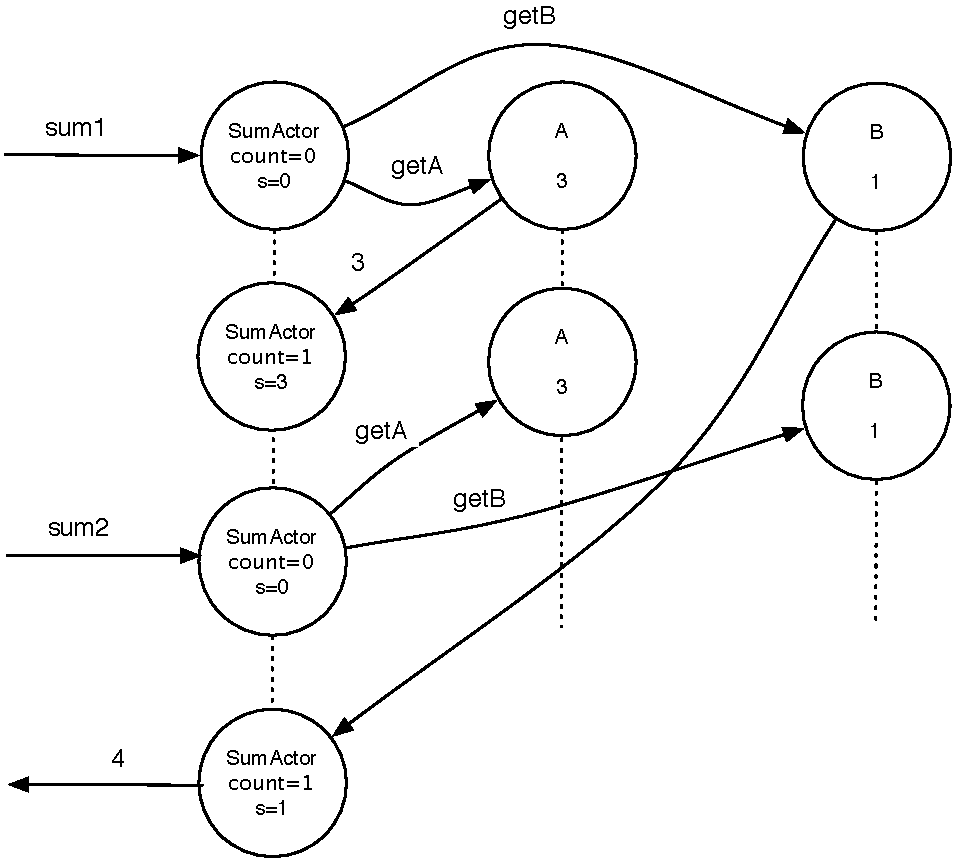
\includegraphics[width=8cm]{4-ProposedFramework/Figures/ExampleCoord2.pdf}
    \end{center}
    \caption{\label{fig:coord2} مشکل پیغام‌های همروند در همکاری اکتورها برای پاسخ به درخواست مجموع a و b}
\end{figure*}
مثال فوق نشان می‌دهد که در طراحی به روش تبادل ناهمگام پیغام در صورتی که نیاز به همکاری بین اکتورها وجود داشته باشد ممکن است درخواست‌های همروند موجب تداخل در محاسبات همدیگر بشوند. این مشکل زمانی پیش می‌آید که شرایط زیر برقرار باشند:\\
 \begin{enumerate}
 \item برای پاسخ به یک درخواست، اکتور مجبور به همکاری با سایر اکتورها باشد.
 \item همکاری به ارسال پیغام به سایر اکتورها ختم نشود و در ادامه لازم باشد پاسخ آنها دریافت شود. 
 \item ارسال پیغام‌ها به صورت ناهمگام انجام شود. به این معنی که اکتور مورد نظر پس از ارسال پیغامهای مربوطه بتواند بدون توقف برای دریافت پاسخ‌ها به پردازش سایر پیغام‌ها بپردازد.
 \item اکتور با دریافت هر کدام از پاسخ‌ها متغیر(های) محلی خود را بروزرسانی کند.
 \end{enumerate}
راه حل مشکل:\\
برای حل این مشکل در زمان طراحی چند گزینه پیش رو داریم:
\begin{itemize}
\item گزینه‌ی اول این است که به جای ارسال ناهمگام پیغام‌های مربوط به یک درخواست، عمل تبادل پیغام را به صورت همگام انجام دهیم. در این حالت اطمینان حاصل می‌شود که درخواست جدید قبل از اتمام عملیات درخواست قبلی پردازش نمی‌شود. ایراد این روش این است که باعث محدودیت در همروندی سیستم می‌گردد.
\item راه دوم این است که به گونه‌ای متغیرهای حالت را نگهداری کنیم که با پردازش درخواست‌های همروند دچار مشکل نشوند. برای این کار نیاز داریم تا متغیرهای حالت را برای درخواست‌های پردازش شده اختصاصی کنیم. در مثال معرفی شده در  شکل \ref{fig:coord1} این کار به این صورت انجام می‌شود که به جای متغیر‌های s و count برای هر درخواست متغیر جدیدی در نظر بگیریم. طبیعتاً این روش منجر به ایجاد پیچیدگی در زمان پیاده‌سازی می‌شود و تضمین محافظت از متغیرها کار دشواری خواهد بود.
\item
 راه مناسب برای حل این مشکل این است که تمام عملیات مربوط به درخواست دریافت شده، به یک اکتور دیگر که فقط وظیفه‌ی پاسخ به این درخواست را دارد منتقل شود. به این روش هم مشکل متغیر‌های حالت محلی به وجود نمی‌آید و هم همروندی سیستم محدود نمی‌شود. طبیعتاً برای جلوگیری از تکرار همین مشکل برای اکتور جدید باید به ازای هر درخواست مشابه یک نمونه‌ی جدید از اکتور مذکور ایجاد کنیم.\\
بنابراین در طراحی به روش تبادل ناهمگام پیغام علاوه‌ بر جلوگیری از پیچیدگی و بزرگ شدن بیش از حد کلاس، ممکن است به دلیل ایجاد امکان پردازش درخواست‌های همروند نیز تصمیم به واگذاری درخواست به اکتوری جدید نماییم.
 در طراحی سیستم آموزش که در بخش‌های قبل توضیح داده شد، در موارد متعددی از جمله در مورد کاربرد محاسبه‌ی معدل (بخش \ref{gpa_approch2}) این الگو مشاهده شد.

\end{itemize}
\item\textbf{پردازش پیغام بدون همکاری با سایر اکتورها}\\
 مستقل از این موضوع که پردازش یک درخواست توسط خود اکتور انجام می‌شود یا به اکتور جدیدی منتقل می‌شود، در طراحی سیستم باید مشخص شود که منطق مربوط به یک درخواست چگونه پیاده‌سازی خواهد شد. ساده‌ترین حالت برای اجرای منطق مربوط به یک درخواست این است که اکتور دریافت کننده، بتواند بدون همکاری با سایر اکتورها عملیات لازم را انجام دهد و در صورت لزوم پاسخ درخواست را ارسال کند. این حالت زمانی رخ می‌دهد که اکتور تمام اطلاعات لازم برای اجرای منطق مربوطه را در حالت خود داشته باشد.
 در این حالت اکتور پس از دریافت پیغام، منطق مربوط به آن را انجام می‌دهد و در صورت لزوم پاسخ مناسب را برای مقصد ارسال می‌کند. ممکن است حالت اکتور پس از  پردازش این پیغام تغییر کند. شکل \ref{fig:no_collaboration} این حالت را نشان می‌دهد.
 \begin{figure*}[h]
    \begin{center}
	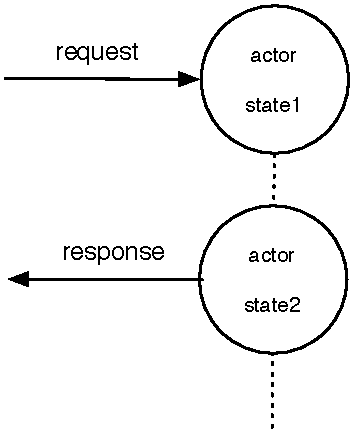
\includegraphics[width=6cm]{4-ProposedFramework/Figures/NoCollaboration.pdf}
    \end{center}
    \caption{\label{fig:no_collaboration} پردازش پیغام بدون همکاری با سایر اکتورها}
\end{figure*}

\item\textbf{پردازش پیغام به وسیله‌ی همکاری با سایر اکتورها}\\
اینجا می‌گم در چه حالت‌هایی باید همکاری کنیم و چه تصمیم‌هایی بگیریم. مثلا این که سینک باشه یا ایسینک

\end{itemize}
%
%
%%تا این مرحله از طراحی، مشخص شده است که اکتور مسئول برای دریافت پیغام کدام است. در طراحی شیءگرای ترتیبی در این مرحله شیء دریافت کننده‌ی درخواست با دو حالت زیر روبرو می‌شود:\\
%%\begin{itemize}
%%\item شیء مورد نظر با توجه به داده‌های محلی که در اختیار دارد می‌تواند بدون همکاری سایر اشیاء عملیات مربوط به درخواست را انجام بدهد. در این حالت شیء مورد نظر عملیات لازم را انجام می‌دهد و درصورتی که درخواست نیاز به پاسخ داشته باشد جواب را به صورت مقدار بازگشت متد\LTRfootnote{return value} ارسال می‌کند. 
%%\item در حالتی که شیء مورد نظر به تنهایی قادر به پردازش درخواست نباشد، به فراخوانی متدهای اشیاء دیگر می‌پردازد و نهایتاً عملیات مورد نظر انجام‌ می‌شود. در این حالت ممکن است در طول برقراری ارتباط با سایر اشیاء، حالت درونی شیء (داده‌ها محلی) برای نگهداری وضعیت پردازش درخواست تغییر کند.
%%\end{itemize}
% بنابراین این اکتور وظیفه‌ی پردازش پیغام را بر عهده دارد. یک اکتور برای پردازش پیغام چند راهکار پیش رو دارد:\\
%\begin{itemize}
%\item حالت اول این است که اکتور با توجه به داده‌های محلی که در اختیار دارد، بتواند تمام پردازش‌ها مربوط به درخواست دریافت شده را بدون نیاز به ارتباط با سایر اکتورها انجام دهد. طبیعتاً در این حالت ساده‌ترین راه برای پردازش پیغام این است که خود اکتور عملیات لازم برای پاسخ به درخواست را انجام داده و پاسخ نتیجه را ارسال کند.
%
%\item حالت دیگر زمانی است که اکتور به تنهایی قادر به پاسخ‌گویی به پیغام نباشد و برای تهیه‌ی نتیجه نیاز به برقراری ارتباط با سایر اکتورها داشته باشد. در این حالت نیز اکتور دو رویکرد را می‌تواند اتخاذ کند: رویکرد اول این است که خود اکتور اقدام به ارسال پیغام‌های لازم برای اکتورهای مرتبط کند و پاسخ‌های آنها را دریافت کرده و نتیجه‌ی عملیات را مشخص کند. رویکرد دوم این است که کل عملیات پردازش این پیغام را به اکتور دیگری واگذار کند. با اینکه این 
%
%\end{itemize}
\end{enumerate}












\section{الگوهای طراحی استخراج شده و نکات مهم}
در این بخش الگوهای طراحی و نکات مهمی‌ که در طول انجام طراحی موارد کاربرد به دست آمده است گردآوری و ارائه شده است. نحوه‌ی تقسیم‌بندی موارد این بخش به این صورت است که ابتدا الگوهای  کلی همکاری اکتورها برای پیاده‌سازی منطق دامنه برشمرده شده‌اند و برای هر مورد سعی شده تأثیر منطق دامنه در انتخاب الگو و نیز در نحوه‌ی پیاده‌سازی جزئیات الگو در نظر گرفته شود. در ادامه الگوها و نکته‌های مهم در طراحی پیغام‌ها ارائه شده‌اند. نهایتا نکات و تجربیاتی که در زمینه‌ی طراحی به روش انتقال ناهمگام و تفاوت‌های مهم آن با طراحی شیءگرای ترتیبی ارائه شده است.
\subsection{الگوهای همکاری اکتورها}
\subsubsection{الگوی انشعاب و الحاق}

\begin{itemize}
\item\textbf{نحوه‌ی پیاده‌سازی به روش تبادل ناهمگام پیغام:}\\
همان‌طور که از نام این الگو بر می‌آید پیاده‌سازی آن از دو بخش تشکیل شده است. برای عمل انشعاب یک اکتور به تعدادی اکتور دیگر که به آنها دسترسی دارد و یا خود آنها را ایجاد می‌کند پیغام‌هایی می‌فرستد. این اکتورها تمام عملیات لازم برای تهیه‌ی پاسخ را انجام داده و پیغام‌های پاسخ را برای اکتور اصلی ارسال می‌کنند. مرحله‌ی جمع‌آوری پیغام‌ها انشعاب نامیده می‌شود. اکتور اصلی این پیغام‌‌ها را دریافت کرده و محاسبات لازم را روی آنها انجام می‌دهد. و در پاسخ عملیات را به صورت پیغام ارسال می‌کند.‍ شکل \ref{fig:fork_and_join} شمایی از این الگو را نشان می‌دهد.
\begin{figure*}
    \begin{center}
	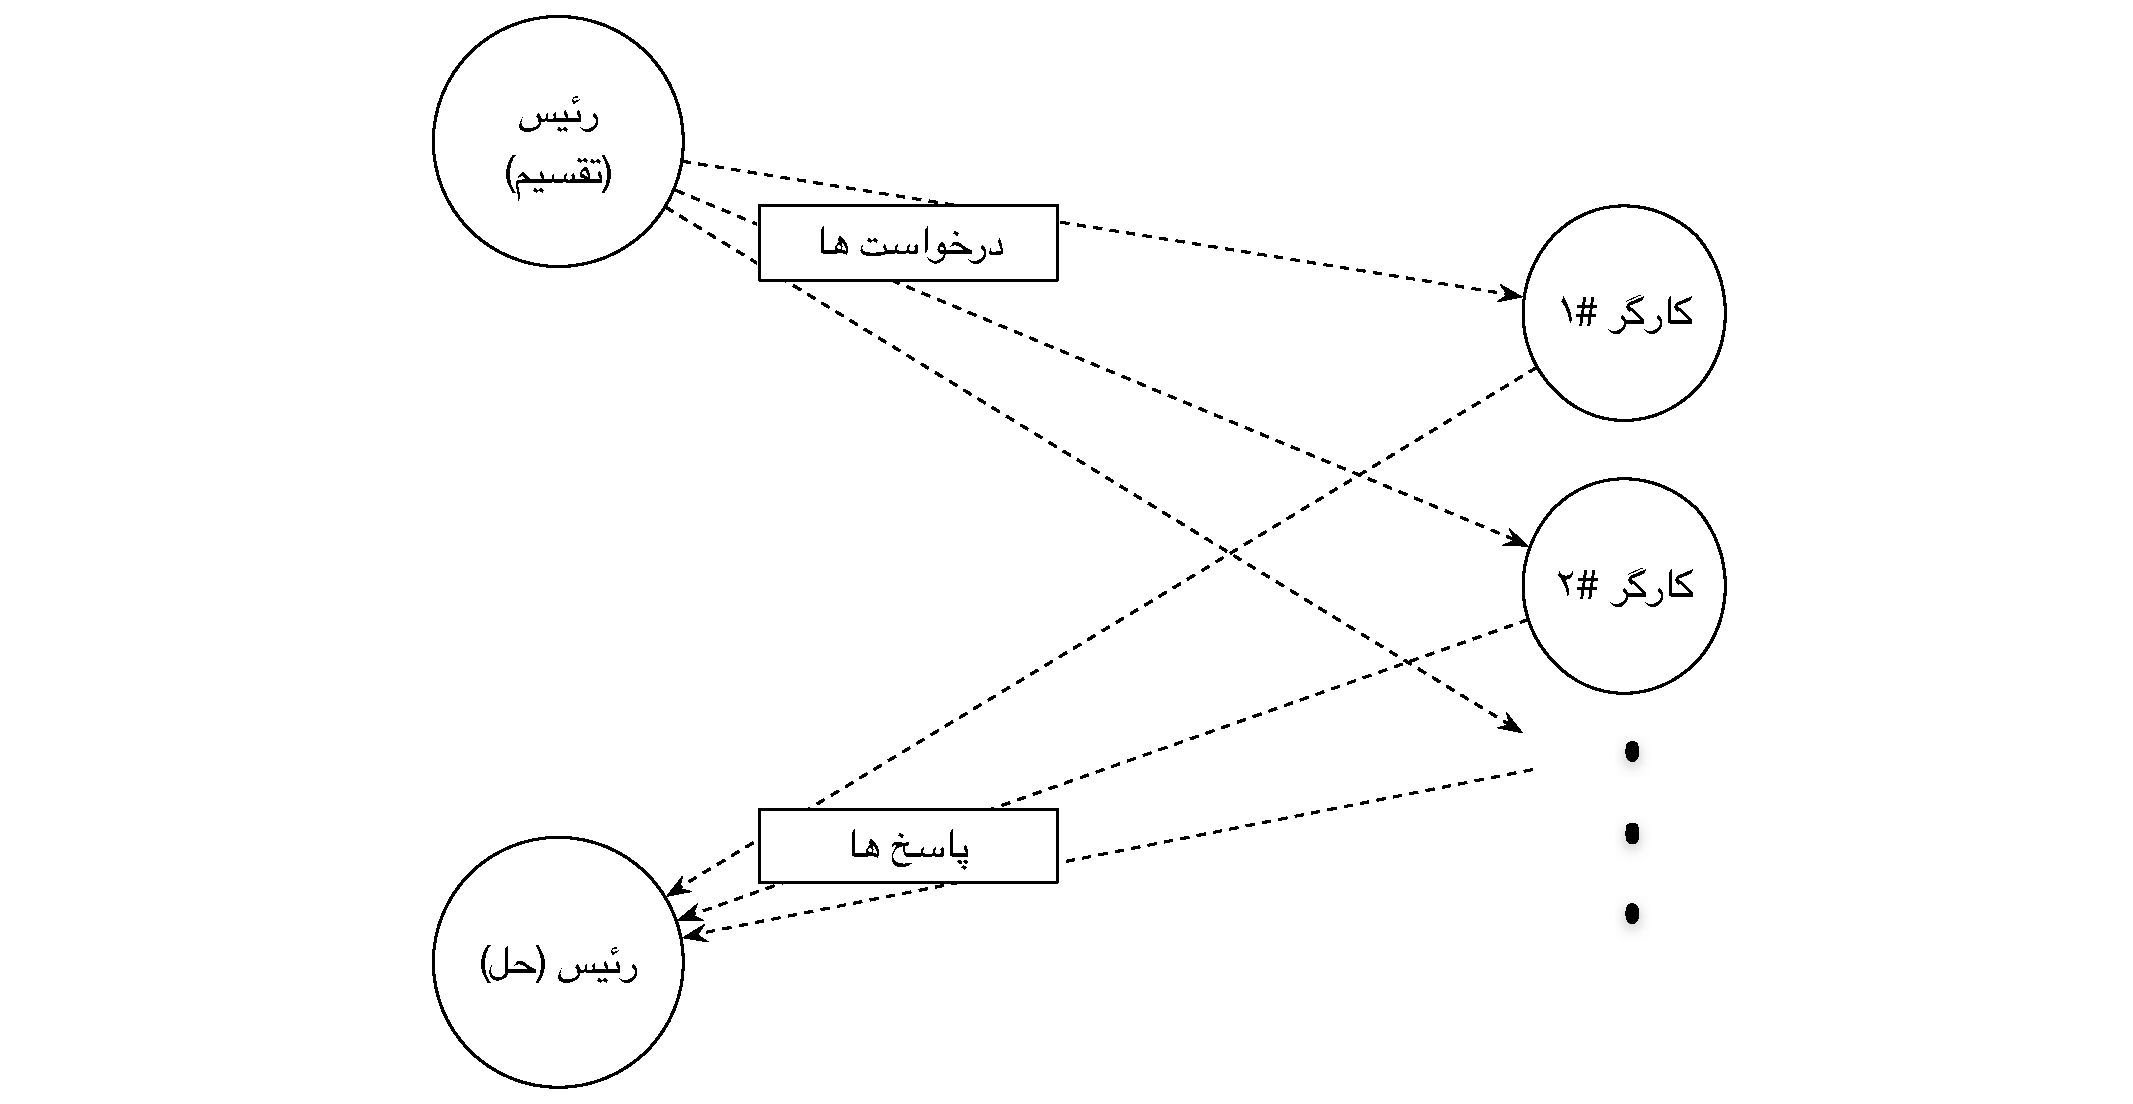
\includegraphics[width=16cm]{3-RelatedWork/Figures/Divide_and_Conquer.pdf}
    \end{center}
    \caption{\label{fig:fork_and_join}  شمای کلی از الگوی انشعاب و الحاق در مدل اکتور }
\end{figure*}

\item\textbf{موارد استفاده}\\
این الگو برای حالاتی از منطق دامنه به کار می‌رود که مسئله از نوع تقسیم و حل است (رجوع کنید به بخش \ref{section:actorPatterns}). مثالی از این کارکرد در مورد کاربرد محاسبه‌ی معدل (جدول \ref{table:uc_gpa}) در بخش قبل مورد بررسی قرار گرفته است. در این مثال، اکتوری که وظیفه‌ی محاسبه‌ی معدل را بر عهده دارد به اکتورهای سابقه‌ی تحصیلی دانشجو دسترسی دارد و برای محاسبه‌ی معدل نیاز به اطلاعاتی دارد که این اکتورها به آن دسترسی دارند. استفاده از الگوی انشعاب و الحاق در این مثال به این صورت است که اکتور محاسبه‌ی معدل پیغام‌های درخواست اطلاعات نمره را برای تمام اکتورهای سابقه ارسال می‌کند (انشعاب)، این اکتورها با برقراری ارتباط با سایر اکتورها موجب می‌شوند اطلاعات لازم به صورت پیغام‌هایی برای اکتور محاسبه‌ی معدل ارسال شود. اکتور محاسبه‌ی معدل با گرفتن پیغام‌ها (الحاق) عملیات مورد نیاز برای محاسبه‌ی معدل را انجام‌ می‌دهد و معدل را به صورت پیغام برای اکتور مقصد ارسال می‌کند.
%موارد استفاده‌ی دیگری هم دارد.؟

\item\textbf{نکات مهم}\\
\begin{enumerate}
\item مناسب بودن مسائل تقسیم و حل برای این الگو به این معنی نیست که نمی‌توان از روش دیگری این مسائل را حل کرد. به عنوان مثال، مورد کاربرد محاسبه‌ی معدل در رویکرد  اول طراحی که در بخش \ref{gpa_approach1} توضیح داده شد، بدون استفاده از این الگو طراحی گردید. همان‌طور که در مقایسه‌ی دو رویکرد مذکور بیان شد، تفاوت استفاده و عدم استفاده از الگوی انشعاب و الحاق صرفا کیفیت طراحی می‌باشد و از نظر صحت عملکرد دو الگو یکسان هستند. بنابراین استفاده از این الگو بیشتر به تمرین در طراحی نیازمند است و صرفاً از روی منطق دامنه قابل تشخیص نیست.
\item مورد دیگر این است که در بسیاری از موارد، استفاده از این الگو به ذهن برنامه‌نویس این طور القا می‌کند که اکتورهایی که انشعاب شده‌اند موظف به فرستادن نتیجه به اکتور اصلی هستند. باید دقت شود که استفاده از این الگو مستقل از این مورد است که نتیجه‌ی کارهای تقسیم شده به چه شکلی به دست اکتور اصلی می‌رسد. همان‌طور که در رویکرد دوم طراحی مورد کاربرد محاسبه‌ی معدل مشاهده شد، پاسخ اکتور محاسبه‌ی معدل می‌تواند از سوی اکتور ترم و یا اکتور درس ارسال شود.
\item استفاده از این الگو صرفا با کشف مورد استفاده به اتمام نمی‌رسد. پس از تصمیم به استفاده از این الگو، تصمیمات دیگری در پاسخ به سؤالاتی از این قبیل باید اتخاذ شود: آیا  اکتور جاری که منطق مطابق با الگو در آن کشف شده است باید به عنوان اکتوری که انشعاب در نظر گرفته شود یا اکتور دیگری به این منظور ایجاد شود؟ آیا اکتور الحاق و اکتور انشعاب یکسان باشند یا اکتور دیگری عمل انشعاب را انجام دهد؟ آیا نتیجه‌ی عملیات حاصل از الگو به اکتور جاری فرستاده شود یا مستقیماً به گیرنده‌ی دیگری ارسال شود؟ 
\end{enumerate} 

\end{itemize}

\subsubsection{الگوی خط لوله}

\begin{itemize}
\item\textbf{نحوه‌ی پیاده‌سازی به روش تبادل ناهمگام پیغام:}\\
پیاده‌سازی این الگو به این صورت است که هر اکتور بخشی از عملیات منطق دامنه‌ را انجام می‌دهد و با ارسال پیغام به اکتور بعدی ادامه‌ی کار را به آن می‌سپارد.
\begin{figure*}
    \begin{center}
	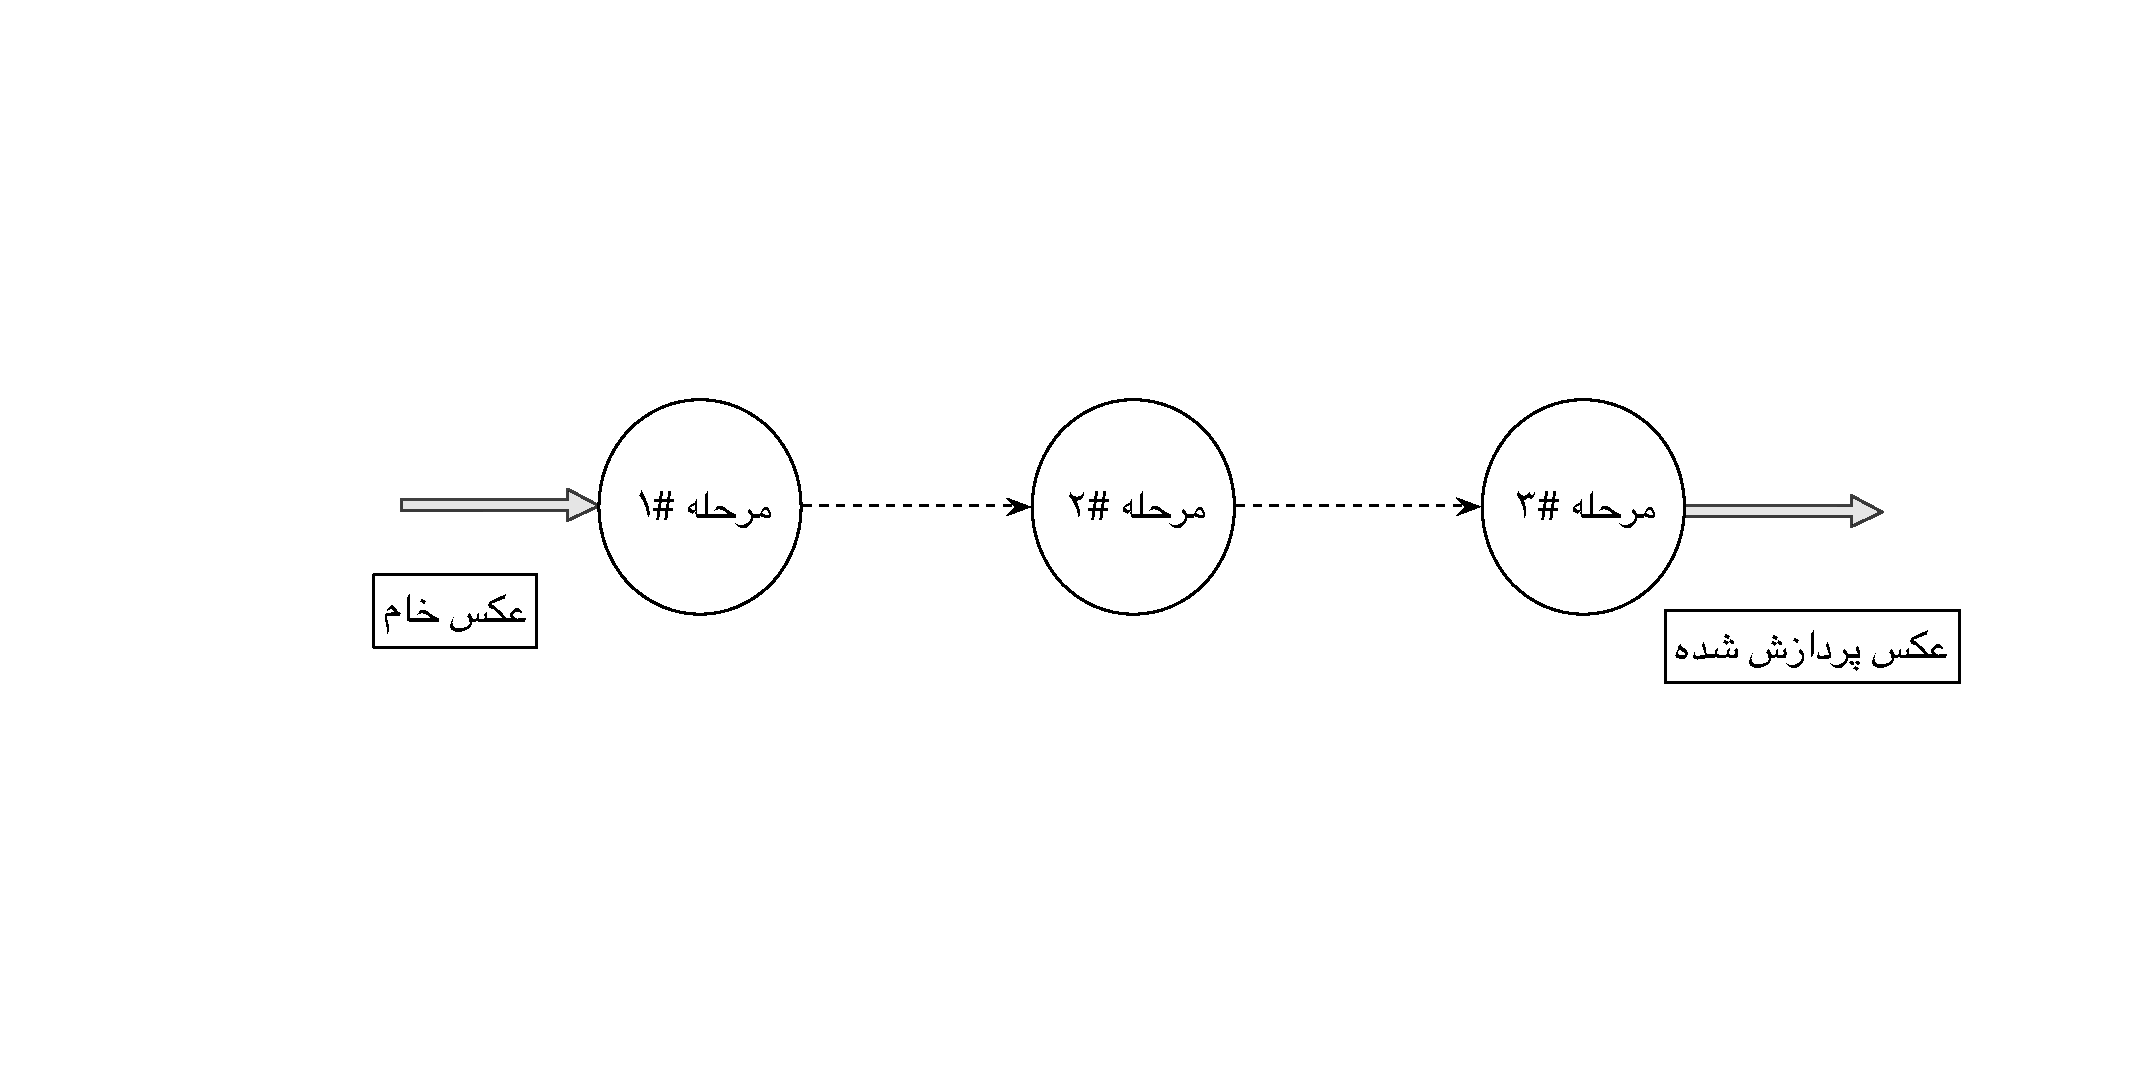
\includegraphics[width=16cm]{3-RelatedWork/Figures/pipeline.pdf}
    \end{center}
    \caption{\label{fig:pipeline_2}  مثالی از الگوی خط لوله }
\end{figure*}

\item\textbf{موارد استفاده}\\
این الگو در دو حالت مورد استفاده قرار می‌گیرد. حالت اول مواردی را شامل می‌شود که خود منطق دامنه نیاز به ترتیب دارد. در این حالت‌ها عملی که در هر مرحله انجام‌ می‌گیرد به صورت منطقی وابسته به نتیجه‌ی مرحله‌ی قبل است. حالت دوم زمانی اتفاق می‌افتد که منطق دامنه نیاز به ترتیب ندارد ولی دسترسی اکتورها به صورت زنجیره‌ای است. مثالی از این حالت،‌ در مورد کاربرد محاسبه‌ی معدل در بخش قبل دیده شد. در این مثال اکتور سابقه، نمره‌ی دانشجو را برای معدل فراهم می‌کند و اکتور درس تعداد واحد‌های درس مربوطه را. با اینکه این دو عمل مستقل از هم بوده و می‌توانند به صورت موازی اجرا شوند،‌ مدل دامنه‌ی سیستم ایجاب می‌کند که پیغام از طریق اکتور سابقه به اکتور ارائه منتقل شود و از طریق این اکتور به دست اکتور درس برسد.

\item\textbf{نکات مهم}\\
\begin{enumerate}
\item مناسب بودن م\textsl{سائل تقسیم و حل} برای این الگو به این معنی نیست که نمی‌توان از روش دیگری این مسائل را حل کرد. به عنوان مثال، مورد کاربرد محاسبه‌ی معدل در رویکرد  اول طراحی که در بخش \ref{gpa_approach1} توضیح داده شد، بدون استفاده از این الگو طراحی گردید. همان‌طور که در مقایسه‌ی دو رویکرد مذکور بیان شد، تفاوت استفاده و عدم استفاده از الگوی انشعاب و الحاق صرفا کیفیت طراحی می‌باشد و از نظر صحت عملکرد دو الگو یکسان هستند. بنابراین استفاده از این الگو بیشتر به تمرین در طراحی نیازمند است و صرفاً از روی منطق دامنه قابل تشخیص نیست.
\item مورد دیگر این است که در بسیاری از موارد، استفاده از این الگو به ذهن برنامه‌نویس این طور القا می‌کند که اکتورهایی که انشعاب شده‌اند موظف به فرستادن نتیجه به اکتور اصلی هستند. باید دقت شود که استفاده از این الگو مستقل از این مورد است که نتیجه‌ی کارهای تقسیم شده به چه شکلی به دست اکتور اصلی می‌رسد. همان‌طور که در رویکرد دوم طراحی مورد کاربرد محاسبه‌ی معدل مشاهده شد، پاسخ اکتور محاسبه‌ی معدل می‌تواند از سوی اکتور ترم و یا اکتور درس ارسال شود.
\item استفاده از این الگو صرفا با کشف مورد استفاده به اتمام نمی‌رسد. پس از تصمیم به استفاده از این الگو، تصمیمات دیگری در پاسخ به سؤالاتی از این قبیل باید اتخاذ شود: آیا  اکتور جاری که منطق مطابق با الگو در آن کشف شده است باید به عنوان اکتوری که انشعاب در نظر گرفته شود یا اکتور دیگری به این منظور ایجاد شود؟ آیا اکتور الحاق و اکتور انشعاب یکسان باشند یا اکتور دیگری عمل انشعاب را انجام دهد؟ آیا نتیجه‌ی عملیات حاصل از الگو به اکتور جاری فرستاده شود یا مستقیماً به گیرنده‌ی دیگری ارسال شود؟ 
\end{enumerate} 

\end{itemize}

\chapter{ارزیابی}
\label{chapter:evaluation}
\thispagestyle{plain}
\section{مقدمه}
در فصل‌های قبل روش طراحی منطق دامنه بر اساس تبادل ناهمگام پیغام ارائه شد و برخی از الگوهای طراحی در این روش به همراه نکات مهم آن مورد بررسی قرار گرفت. در این فصل دو معیار کیفی تغییرپذیری و کارایی در طراحی به این روش مورد ارزیابی قرار می‌گیرد. برای انجام ارزیابی ابتدا سیستم معرفی شده در بخش \ref{section:eduIntro} بر اساس طراحی ارائه شده، پیاده سازی شده است. با توجه به اینکه قضاوت در مورد معیارهای انتخاب شده برای بررسی، در مقایسه با رویکرد طراحی شیءگرا مفهوم پیدا می‌کند سیستم مذکور توسط روش متداول شیءگرا نیز طراحی و پیاده‌سازی شده است. در پیاده‌سازی نسخه‌ی شیءگرا از الگوی مدل دامنه \cite{Fowler_Patterns} برای لایه‌ی منطق دامنه بهره گرفته شده است. ضمناً به هدف نزدیکتر شدن سیستم معرفی شده به پیاده‌سازی‌های واقعی، امکان ماندگاری\LTRfootnote{persistence} داده‌ها در پایگاه داده نیز به هر دو طراحی افزوده گردیده است. در هر دو پیاده‌سازی از الگوی \gls{مخزن}\LTRfootnote{repository}\cite{Fowler_Patterns} برای نگاشت اشیاء دامنه به جداول پایگاه داده استفاده شده است.
با توجه به حجم بالای برنامه‌های پیاده‌سازی شده و نیز به هدف قابلیت استفاده‌، متن برنامه‌ی تولید شده به هر دو روش به همراه کتابخانه‌های لازم برای اجرا، به صورت برخط در دسترس عموم قرار داده شده‌ است\cite{sources_java,sources_scala}. جهت حفظ دقت مقایسه تلاش شده است تا دو طراحی از نظر کارکرد حداکثر شباهت با یکدیگر را داشته باشند. برای پیاده‌سازی سیستم به روش طراحی بر اساس تبادل ناهمگام پیغام، از کتابخانه‌ی اکتور اسکالا استفاده شده و برای پیاده‌سازی به روش شیءگرا از زبان جاوا استفاده شده است. در پایان این قسمت یادآوری می‌شود که تحلیل دقیق و عمیق دلیل اختلاف‌های احتمالی در معیارهای مقایسه شده بین دو روش در حوزه‌ی این پژوهش نیست و هدف از انجام این ارزیابی صرفاً قیاس دو روش از نظر معیارهای انتخاب شده است.
\section{روش ارزیابی}
\label{section:gqm}
در این ارزیابی از روش \textit{هدف-پرسش-معیار}\LTRfootnote{Goal-Question-Metric} استفاده شده است. هدف-پرسش-معیار یک روش نظام‌مند برای تعیین معیارهای ارزیابی متناسب با دامنه‌ی مسئله است. این روش یک رویکرد بالا-به-پایین\LTRfootnote{top-down} است که از قدم‌های زیر تشکیل می‌شود:\cite{GQM}
\begin{enumerate}
\item تعیین هدف: به این پرسش پاسخ می‌دهد که \textbf{هدف} از اندازه‌گیری  و ارزیابی چه چیزی است.
\item قدم بعدی تعریف \textbf{پرسش‌}هایی است که اگر پاسخ آنها داده شود هدف اندازه‌گیری برآورده می‌شود.
\item برای پاسخ کمّی به پرسش‌هایی که تعریف شده‌اند، به هر پرسش دسته‌ای از \textbf{معیار}ها تخصیص داده می‌شود.
\end{enumerate}

\begin{figure*}[htb]
    \begin{center}
	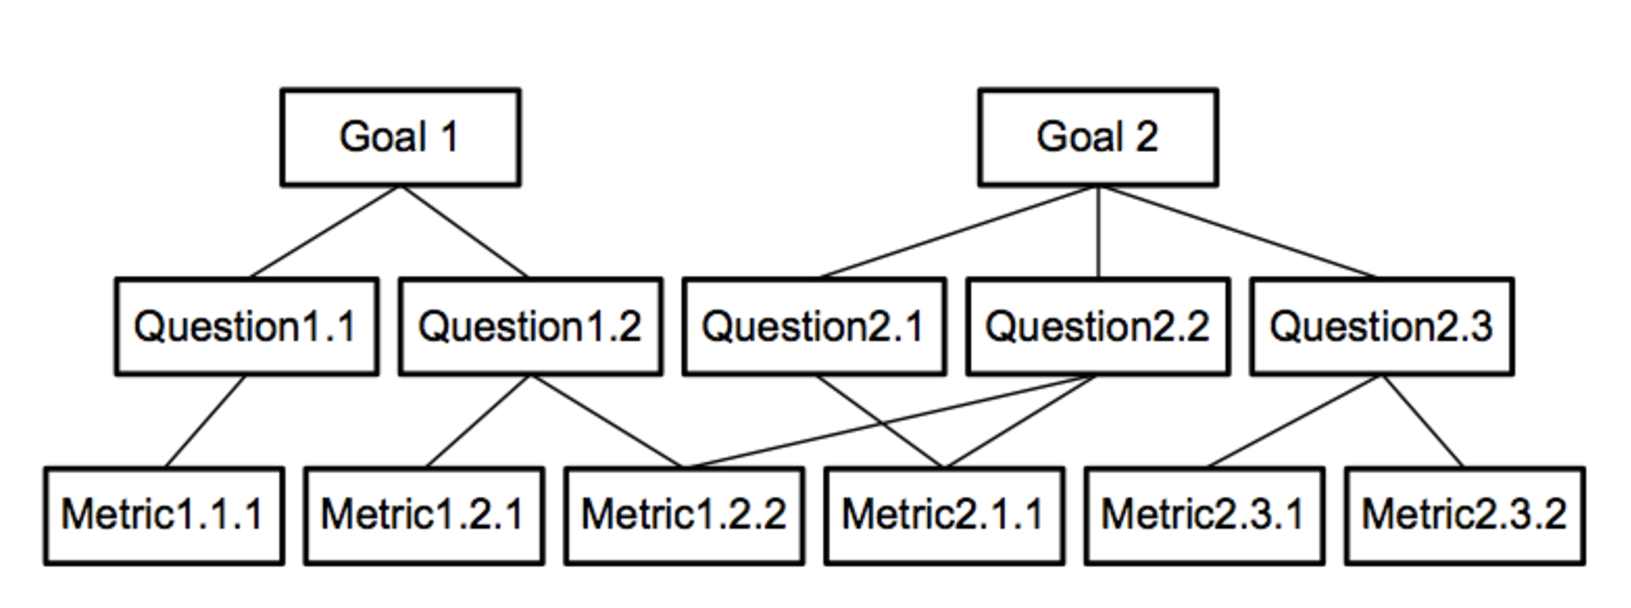
\includegraphics[width=10cm]{5-Evaluation/Figures/gqm.pdf}
    \end{center}
    \caption{\label{fig:gqm} ساختار روش هدف-پرسش-معیار }
\end{figure*}

\section{ارزیابی تغییرپذیری}
در این بخش به ارزیابی تغییرپذیری سیستم تحت طراحی بر اساس تبادل ناهمگام پیغام می‌پردازیم. برای ایجاد امکان ارزیابی کمّی تغییرپذیری، می‌توان از معیارهای کیفیت نرم‌افزار\LTRfootnote{Software Quality Metrics} استفاده کرد. این معیارها خصوصیاتی از قبیل پیچیدگی، قابلیت استفاده‌ی مجدد و آزمون‌پذیری یک سیستم را به صورت کمّی قابل سنجش و مقایسه می‌کنند. در ادامه با توجه به روش هدف-پرسش-معیار، عناصر ارزیابی تغییرپذیری سیستم را تعیین می‌کنیم.

\subsection{هدف}
در این ارزیابی هدف ارزیابی تغییرپذیری طراحی به روش تبادل ناهمگام پیغام است. این ارزیابی از طریق مقایسه‌ی نسخه‌های پیاده سازی شده‌ی سیستم آموزش ساده (بخش \ref{section:eduIntro}) به دو روش طراحی تبادل ناهمگام پیغام و طراحی متداول شیءگرا صورت می‌پذیرد.

\subsection{پرسش‌ها}
برای این ارزیابی ۳ پرسش در نظر گرفته می‌شود:
\begin{enumerate}
\item سیستم طراحی شده به روش تبادل ناهمگام، از نظر معیارهای کیفیت نرم‌افزار چگونه با سیستم طراحی شده به روش شیءگرا مقایسه می‌شود؟
\item اعمال تغییر قواعد منطق برنامه\LTRfootnote{business rules} روی کدام نوع طراحی مشکل‌تر است؟ 
\item اعمال تغییر در مدل دامنه‌ی سیستم روی کدام نوع طراحی مشکل‌تر است؟ 
\end{enumerate}

\subsection{معیارها}
% به منظور پاسخ به هر کدام از پرسش‌های بالا می‌توان از معیارهای کیفیت در برنامه‌نویسی شیءگرا  استفاده کرد. پاسخ به پرسش اول مستقیماً با مقایسه‌ی معیارها پاسخ داده می‌شود. برای پرسش به پاسخ دوم، تغییرات منطق دامنه انتخاب و در هر دو سیستم اعمال می‌شوند و میزان تغییر هر کدام از معیارهای کیفیت بررسی و مقایسه می‌شود. برای پاسخ به پرسش سوم نیز به طریق مشابه می‌توان مقایسه را بعد از اعمال تغییر در مدل دامنه انجام داد. 
در پژوهش‌های مختلف، معیارهای مختلفی برای بررسی کیفیت برنامه‌های شیءگرا ارائه شده‌اند که از آن جمله می‌توان به معیارهای ابریو\LTRfootnote{Abreu}\cite{quality_metrics_1,quality_metrics_2}، معیارهای بانسیا و همکاران\LTRfootnote{Bansia et al}\cite{quality_metrics_3} و معیارهای چیدامبر و کمرر\LTRfootnote{Chidamber and Kemerer} (که به متریک‌های سی‌کِی معروف هستند) اشاره کرد \cite{quality_metrcs_ck}. در این پژوهش تعدادی از متریک‌های موجود برای ارزیابی انتخاب شده‌اند. این انتخاب بر اساس میزان ارجاع در پژوهش‌های مختلف به این متریک‌ها و نیز تناسب آنها با طراحی‌های این پژوهش انجام شده است. مقاله‌ی \cite{metrics_stateOfTheArt} اطلاعات کاملی از متریک‌های مختلف کیفیت نرم‌افزار و میزان ارجاع به آنها را ارائه کرده است. معیارهای انتخاب شده برای پرسش اول، در ادامه معرفی شده‌اند. در تعاریف و توضیحات این معیارها از مقاله‌ی \cite{metrics_stateOfTheArt} بهره گرفته شده است.
\begin{enumerate}
\item\textbf{تعداد کلاس:}
 تعداد کلاس‌های پیاده‌سازی شده (بدون در نظر گرفتن کلاس‌های داخلی)
\item\textbf{میانگین تعداد متد در هر کلاس}

\item\textbf{میانگین تعداد فیلد تعریف شده در هر کلاس}

\item\textbf{تعداد خطوط متن برنامه}

\item\textbf{میانگین تعداد خطوط متن هر کلاس}

\item\textbf{میانگین پیچیدگی چرخه‌ای \lr{(CC)}\LTRfootnote{Average Cyclomatic Complexity}:}
پیچیدگی چرخه‌ای یک متد برابر است با تعداد نقاط تصمیم در گراف کنترل آن بعلاوه‌ی یک. نقاط تصمیم در یک متد در شرط‌ها و حلقه‌ها و دستورهای مشابه رخ می‌دهند. به عنوان مثال، پیچیدگی چرخه‌ای برای یک متد که یک بلوک شرط \lr{(if)} یا یک حلقه دارد عدد ۲ است و برای متدی که صرفاً دستورات خطی دارد عدد ۱ است. هرچه عدد پیچیدگی چرخه‌ای بزرگتر باشد برنامه به موارد آزمون بیشتری نیاز دارد.
\item\textbf{میانگین متدهای وزن‌دار در کلاس\LTRfootnote{Average Weighted Methds per Class}:}
تعداد متدهای وزن‌دار در یک کلاس برابر است با جمع پیچیدگی چرخه‌ای متدهای آن کلاس.
\item\textbf{میانگین عمق درخت وراثت \lr{(DIT)}\LTRfootnote{Average Depth of Inheritance Tree}:}
عمق درخت وراثت برابر است با تعداد کلاس‌هایی که در زنجیره‌ی وراثت یک کلاس آن را به ریشه می‌رساند.

\item\textbf{میانگین تعداد فرزندان:}
تعداد فرزندان یک کلاس برابر است با تعداد کلاس‌هایی که در زنجیره‌ی وراثت کلاس پایین‌تر از خود کلاس هستند.
\item\textbf{میانگین \gls{جفت‌شدگی}\LTRfootnote{Coupling} بین اشیاء:}
یک کلاس با کلاس دیگر جفت‌شدگی دارد اگر یکی از دو کلاس (یا هردو) متدی از دیگری را فراخوانی کرده باشد. معیار جفت‌شدگی بین اشیاء برای یک کلاس برابر است با تعداد کلاس‌های که با کلاس مورد نظر جفت‌شدگی دارد. (معیار انتخاب شده میانگین این عدد در بین همه‌ی کلاس‌ها است.)
\end{enumerate}
پرسش‌های دوم و سوم مربوط به اعمال تغییرات در قواعد منطق دامنه و مدل دامنه‌ی سیستم می‌باشند. برای این پرسش‌ها معیارهای زیر مناسب تشخیص داده شده‌اند:
\begin{enumerate}
\item تعداد خطوط اضافه شده به متن برنامه
\item تعداد کلاس اضافه شده
\item تعداد متد وزن‌دار اضافه شده
\item تعداد کلاس تغییر داده شده
\item تعداد متد تغییر داده شده
\end{enumerate}
\subsection{نتایج ارزیابی}
\subsubsection{پرسش اول}
برای پاسخ به پرسش اول، معیارهای انتخاب شده در پیاده‌سازی‌های سیستم آموزش ساده (بخش \ref{section:eduIntro}) به دو روش تبادل ناهمگام پیغام و شیءگرا محاسبه شده و باهم مقایسه شده‌اند. نتیجه‌ی این مقایسه در جدول \ref{table:mod_result_1} ارائه شده است.


%%%%%%%%%%%%%%%%%%%%%%%%%%%%%
%%%%  Q1 results
%%%%%%%%%%%%%%%%%%%%%%%%%%%%%
\begin{table}[ht]
\small
\begin{center}
\begin{tabular}{|p{7cm}|p{4cm}|p{4cm}|}
	\hline
%	\multicolumn{1}{|p{7cm}}{Header 1} & \multicolumn{1}{p{4cm}}{Header 2} & \multicolumn{1}{p{4cm}|}{Header 3} \\
%\multicolumn{1}{|p{7cm}}{\textbf{معیار}} & \multicolumn{1}{|p{4cm}}{\textbf{مقدار معیار برای طراحی به روش شیءگرا}} & \multicolumn{1}{|p{4cm}|}{\textbf{مقدار معیار برای طراحی به روش تبادل ناهمگام پیغام}} \\
\textbf{معیار} & \textbf{مقدار معیار برای طراحی به روش شیءگرا} & \textbf{مقدار معیار برای طراحی به روش تبادل ناهمگام پیغام} 
\\ 
	\hline
	تعداد کلاس
	 &
	 ۱۵
	 &
 ۱۷
\\
	\hline
	میانگین تعداد متد در هر کلاس
	 &
	 ۶/۲
	 &
	 ۵/۱۱
\\
	\hline
	میانگین تعداد فیلد تعریف شده در هر کلاس
	 &
	 ۱/۹۳
	 &
	 ۲/۱۴
\\
	\hline

	تعداد خطوط متن برنامه
	 &
	 ۶۶۴
	 &
	 ۷۶۰
\\
	\hline
	
		میانگین تعداد خطوط متن هر کلاس
	 &
	 ۴۴/۲۷
	 &
	 ۴۲/۲۲
\\
	\hline
	
		میانگین پیچیدگی چرخه‌ای
	 &
	 ۱/۵۸
	 &
	 ۱/۲۵
\\
	\hline
	
		میانگین متدهای وزن‌دار در کلاس
	 &
	 ۹/۸
	 &
	 ۷/۱۲
\\
	\hline
	
		میانگین عمق درخت وراثت
	 &
	 ۱/۳۳
	 &
	 ۱/۵۹
\\
	\hline
	
		میانگین تعداد فرزندان
	 &
	 ۰/۳۳
	 &
	 ۰/۵۹
\\
	\hline
	
			میانگین جفت شدگی بین اشیاء
	 &
	 ۳/۶
	 &
	 ۳/۱۸
\\
	\hline
\end{tabular}
\caption{\label{table:mod_result_1} مقادیر معیارها برای پرسش اول}
\end{center}
\end{table}
\FloatBarrier
\subsubsection{پرسش دوم}
پرسش دوم مربوط به تغییر در قواعد منطق دامنه است. تغییر انتخاب شده به این نحو است که در مورد کاربرد اخذ درس (بخش \ref{table:uc_takecoure}) یک شرط به شروط لازم برای قبول اخذ درس اضافه می‌کنیم. این شرط مربوط به تعداد واحدهای اخذ شده توسط دانشجو در ترم جاری است. طبق این شرط، اگر تعداد واحدهای اخذ شده توسط دانشجو در ترم جاری با اخذ درس جدید به بیش از ۲۰ واحد برسد اجازه‌ی اخذ درس به دانشجو نمی‌دهیم.\\
نتایج اعمال تغییر ذکر شده در هر کدام از طراحی‌ها با توجه به معیارهای انتخاب شده، در قالب جدول \ref{table:mod_result_2} ارائه شده است.

%%%%%%%%%%%%%%%%%%%%%%%%%%%%%
%%%%  Q2 results
%%%%%%%%%%%%%%%%%%%%%%%%%%%%%

\begin{table}[ht]
\small
\begin{center}
\begin{tabular}{|p{7cm}|p{4cm}|p{4cm}|}
	\hline
\textbf{معیار} & \textbf{مقدار معیار برای طراحی به روش شیءگرا} & \textbf{مقدار معیار برای طراحی به روش تبادل ناهمگام پیغام} 
\\ 
	\hline
	تعداد خطوط اضافه شده به متن برنامه
	 &
	۱۳
	 &
	 ۱۹
\\
	\hline
	تعداد کلاس اضافه شده
	 &
	 ۰
	 &
	 ۱
\\
	\hline
	تعداد متد وزن‌دار اضافه شده
	 &
	 ۴
	 &
	 ۶
\\
	\hline

	تعداد کلاس تغییر داده شده
	 &
	۲
	 &
	 ۲
\\
	\hline

	تعداد متد تغییر داده شده
	 &
	۱
	 &
	 ۲
\\
	\hline

\end{tabular}
\caption{\label{table:mod_result_2} مقادیر معیارها برای پرسش دوم}
\end{center}
\end{table}




\FloatBarrier
\subsubsection{پرسش سوم}
پرسش سوم مربوط به تغییر در اشیاء مدل دامنه است. این پرسش با اعمال دو تغییر در سیستم پاسخ داده شده است:
\begin{enumerate}
\item تغییر اول این است که یک کلاس با عنوان قواعد ترم\LTRfootnote{TermRegulations} به سیستم اضافه می‌شود. وظیفه‌ی این کلاس همان‌طور که از نام آن مشخص است تعیین قواعد یک ترم است. این قواعد شامل مواردی مثل سقف تعداد واحدهای اخذ شده، امکان اخذ مجدد درس و امکان اخذ درس بدون گذراندن پیش‌نیاز می‌شود. ارتباط این کلاس با بقیه‌ی کلاس‌های دامنه به این صورت است که هر شیء ترم، شیء قواعد ترم مربوط به خودش را دارد. فایده‌ی اضافه شدن این کلاس این است که امکان تغییر قوانین در ترم‌های مختلف در سیستم آموزشی به وجود می‌آید. \\
 نتایج اعمال تغییر ذکر شده در هر کدام از طراحی‌ها با توجه به معیارهای انتخاب شده، در قالب جدول \ref{table:mod_result_3_1} ارائه شده است.



%%%%%%%%%%%%%%%%%%%%%%%%%%%%%
%%%%  Q3_1 results
%%%%%%%%%%%%%%%%%%%%%%%%%%%%%

\begin{table}[ht]
\small
\begin{center}
\begin{tabular}{|p{7cm}|p{4cm}|p{4cm}|}
	\hline
\textbf{معیار} & \textbf{مقدار معیار برای طراحی به روش شیءگرا} & \textbf{مقدار معیار برای طراحی به روش تبادل ناهمگام پیغام} 
\\ 
	\hline
	تعداد خطوط اضافه شده به متن برنامه
	 &
	 ۴۳
	 &
	 ۳۴
\\
	\hline
	تعداد کلاس اضافه شده
	 &
	 ۱
	 &
	 ۱
\\
	\hline
	تعداد متد وزن‌دار اضافه شده
	 &
	 ۱۲
	 &
	 ۶
\\
	\hline

	تعداد کلاس تغییر داده شده
	 &
	۲
	 &
	 ۲
\\
	\hline

	تعداد متد تغییر داده شده
	 &
	۳
	 &
	 ۳
\\
	\hline

\end{tabular}
\caption{\label{table:mod_result_3_1} مقادیر معیارها برای پرسش سوم (تغییر اول)}
\end{center}
\end{table}



\item تغییر دوم به این صورت است که به مدل دامنه‌ی سیستم یک کلاس با عنوان برنامه\LTRfootnote{Program} اضافه می‌شود. این کلاس وظیفه دارد پیش‌نیازی بین دروس را تعیین کند. با این تغییر، رابطه‌ی پیش‌نیازی بین دروس حذف می‌شود و پیش‌نیاز بودن یک درس در قالب یک برنامه مشخص می‌شود. هر دانشجو برای تحصیل یک برنامه را انتخاب می‌کند و در آن برنامه مشخص می‌شود که پیش‌نیازهای یک درس کدام دروس هستند.
 نتایج اعمال تغییر ذکر شده در هر کدام از طراحی‌ها با توجه به معیارهای انتخاب شده، در قالب جدول \ref{table:mod_result_3_2} ارائه شده است.

%%%%%%%%%%%%%%%%%%%%%%%%%%%%%
%%%%  Q3_2 results
%%%%%%%%%%%%%%%%%%%%%%%%%%%%%

\begin{table}
\begin{center}
\begin{tabular}{|p{7cm}|p{4cm}|p{4cm}|}
	\hline
\textbf{معیار} & \textbf{مقدار معیار برای طراحی به روش شیءگرا} & \textbf{مقدار معیار برای طراحی به روش تبادل ناهمگام پیغام} 
\\ 
	\hline
	تعداد خطوط اضافه شده به متن برنامه
	 &
	 ۲۸
	 &
	 ۲۷
\\
	\hline
	تعداد کلاس اضافه شده
	 &
	 ۲
	 &
	 ۲
\\
	\hline
	تعداد متد وزن‌دار اضافه شده
	 &
	 ۶
	 &
	 ۶
\\
	\hline

	تعداد کلاس تغییر داده شده
	 &
	۲
	 &
	 ۳
\\
	\hline

	تعداد متد تغییر داده شده
	 &
	۲
	 &
	 ۳
\\
	\hline

\end{tabular}
\caption{\label{table:mod_result_3_2} مقادیر معیارها برای پرسش سوم (تغییر دوم)}
\end{center}
\end{table}

\end{enumerate}


\FloatBarrier
\subsubsection{نتایج ارزیابی}
پیش از بررسی نتایج ارزیابی لازم است تأکید شود که علاوه بر تفاوت طراحی در دو رویکرد مورد مقایسه، عواملی مثل اختلاف زبان پیاده‌سازی و تجربه‌ی طراحی در دو سیستم نیز  می‌تواند باعث ایجاد تفاوت بین معیارهای مورد بررسی در دو رویکرد شود. به همین دلیل اختلاف‌های جزئی در معیارهای بررسی شده قابل چشم‌پوشی هستند.\\
 در ارزیابی پرسش اول مشاهده شد که معیارهای تعداد خط متن برنامه و تعداد کلاس‌ها در حالت تبادل ناهمگام پیغام اندکی بیشتر از  رویکرد طراحی شیءگرا است. بررسی صورت گرفته نشان می‌دهد که افزایش تعداد کلاس‌ها در این رویکرد بیشتر به دلیل استفاده‌ی بیشتر از الگوی وکالت (بخش \ref{pattern:delegate}) در رویکرد طراحی به روش تبادل ناهمگام پیغام است (برای مشاهده‌ی دلیل این امر به بخش  \ref{design:delegate} مراجعه کنید). البته در رویکرد طراحی شیءگرا، برخلاف رویکرد تبادل ناهمگام پیغام، همروندی ذاتی وجود ندارد و به همین دلیل برای ایجاد همروندی، تعدادی کلاس به آن اضافه می‌گردد. سایر معیارها در پرسش اول اختلاف چشم‌گیری باهم ندارند. در ارزیابی پرسش‌ دوم، به طراحی رویکرد تبادل ناهمگام یک کلاس اضافه شده است که دلیل آن همان مورد ذکر شده در فوق می‌باشد. در  ارزیابی پرسش سوم ۲ تغییر در سیستم مورد آزمون قرار گرفت. مقایسه‌ی معیارها نشان می‌دهد که در تغییر اول، طراحی بر اساس تبادل ناهمگام اندکی بهتر از روش شیءگرا عمل کرده است و در تغییر دوم دو سیستم عملکرد مشابهی داشته‌اند. در نهایت با توجه به مقایسه‌ی معیارهای معرفی شده می‌توان نتیجه گرفت که طراحی به روش شیءگرا و تبادل ناهمگام پیغام، در پیاده‌سازی سیستم آموزش ساده، از نظر معیارهای کیفیت معرفی شده عملکرد مشابهی داشته و قابل قیاس با یکدیگر هستند. هرچند اظهار نظر قطعی در مورد مقایسه‌ی  کیفیت طراحی به دو روش مذکور نیازمند بررسی‌ پیاده‌سازی‌های بیشتر و انجام طراحی در دامنه‌های مختلف می‌باشد.

\section{ارزیابی کارایی}
\label{sec:perf}
در این بخش از پژوهش کارایی برنامه‌های طراحی‌ شده به دو روش باهم مقایسه شده‌اند. ارزیابی عمیق و کامل کارایی برنامه، نیاز به بررسی‌های دقیق تمام پارامترهای موثر و انجام آزمایشات گسترده دارد. علاوه بر این برای ارزیابی کارایی سیستم در مواجهه با بار زیاد و همروندی بالا، لازم است مکانیزم‌های پیشرفته‌ی تحمل بار مانند تکنیک‌های \gls{توزین بار}\LTRfootnote{load balancing} و توزیع برنامه در سیستم اعمال گردد. این تکنیک‌ها مستقل از طراحی منطق برنامه، وابسته به استفاده از چارچوب‌ها و کتابخانه‌های مختص این کار است که از حوزه‌ی این پژوهش خارج است. به این دلایل در این ارزیابی، کارایی دو سیستم در آستانه‌ی تحمل بار آزموده نشده است و طبعاً مقادیر به دست آمده برای معیارهای کارایی به معنای حد بالای کارایی دو سیستم نمی‌باشند. علاوه‌ بر این در این ارزیابی، معیارهای کارایی که مربوط به مصرف منابع سیستم هستند (مانند میزان مصرف پردازنده و حافظه) برای مقایسه در نظر گرفته نشده‌اند. البته در طول انجام آزمایش‌ها میزان مصرف منابع پایش شده‌اند تا از عدم  تأثیر اشباع منابع بر نتیجه‌ی آزمایش‌ها اطمینان حاصل شود.\\
برای نزدیک شدن سیستم به پیاده‌سازی‌های واقعی (تجاری)، امکاناتی از قبیل ماندگاری\gls{ماندگاری} داده‌ها در پایگاه داده در پیاده‌سازی هر دو سیستم لحاظ شده‌اند. علاوه بر این، با توجه به اینکه مدل تبادل ناهمگام به دلیل همروندی ذاتی، قادر به پاسخ به درخواست‌های همروند است، برای حفظ اعتبار مقایسه، امکان پردازش همروند درخواست به پیاده‌سازی نسخه‌ی شیءگرا نیز افزوده شده است. این امکان به صورت تخصیص ریسمان به هر درخواست و پردازش کل درخواست در ریسمان تخصیص داده شده صورت گرفته است. به جز موارد فوق، در پیاده‌سازی سیستم مکانیزم ارسال درخواست به سیستم و گرفتن پاسخ و نیز ثبت مقادیر معیارها برای هر درخواست اضافه شده است. با این روش عملکرد کاربران سیستم که در پیاده‌سازی واقعی درخواست‌های خود را از کلاینت‌های سیستم ارسال می‌کنند شبیه‌سازی شده است.

با توجه به این توضیحات، در ادامه هدف و پرسش‌ها و معیارهای انتخاب شده برای ارزیابی کارایی سیستم ارائه شده‌اند و در پایان نتایج ارزیابی به صورت مختصر مورد بررسی قرار گرفته است.
\subsection{هدف}
با توجه به توضیحات ذکر شده، در این ارزیابی، هدف مقایسه‌ی ابتدایی کارایی دو سیستم است که به روش‌های شیءگرا و تبادل ناهمگام پیغام طراحی شده‌اند. 
\subsection{پرسش‌ها}
برای بررسی هدف تعیین شده، پرسش‌های زیر طراحی شده‌اند:
\begin{enumerate}
\item کارایی دو پیاده‌سازی برای درخواستهای همروندی که با توجه به منطق دامنه نرخ ورود آنها به سیستم زیاد است چگونه مقایسه می‌شود؟\\

\item کارایی دو پیاده‌سازی برای درخواستهایی که با توجه به منطق دامنه نرخ ورود آنها به سیستم کم است ولی حجم عملیات آنها گسترده است، چگونه مقایسه می‌شود؟

\end{enumerate}
\subsection{معیارها}
پرسش اول در واقع مربوط به مواردی است که کاربران زیادی به طور همروند اقدام به ارسال درخواست به سیستم می‌کنند. در این موارد دو معیار میانگین زمان پاسخ\LTRfootnote{response time} و نیز \gls{توان عملیاتی}\LTRfootnote{Throughput} معیارهای مناسبی برای اندازه‌گیری هستند\footnote{زمان پاسخ به صورت مدت زمان سپری شده بین ارسال درخواست و دریافت پاسخ تعریف می‌شود و توان عملیاتی به صورت تعداد درخواست‌های موفق در واحد زمان تعریف می‌شود.}.
 در پرسش دوم مسئله‌ای که مورد بررسی قرار می‌گیرد مربوط به درخواست‌هایی است که احتمال ارسال همروند آنها کمتر وجود دارد ولی حجم عملیات مورد نیاز برای پردزاش آنها بیشتر است. با توجه به اینکه این درخواست‌ها به تعداد کم به سیستم ارسال می‌شوند، توان عملیاتی برای این پرسش معیار مناسبی نمی‌باشد. به همین دلیل برای پاسخ به این پرسش فقط از معیار زمان پاسخ استفاده خواهیم کرد.

\subsection{شرایط ارزیابی}
در انجام آزمایش‌های مربوط به ارزیابی کارایی، نکات زیر مورد توجه قرار گرفته‌اند:
\begin{enumerate}
\item انجام آزمایش برای هر دو پیاده‌سازی در شرایط سیستمیِ یکسان صورت گرفته است.
\item در طول انجام آزمایش‌ها از منابع سیستم به طور مرتب مورد پایش قرار گرفته‌اند تا از عدم اشباع منابع و تاثیر آن بر نتایج اطمینان حاصل شود.
\item تمامی اجراها چندین بار تکرار شده‌اند و مقادیر اعلام شده برای معیارها میانگین نتایج آزمایش‌ها هستند.
\item تمام تنظیمات برنامه که بین دو پیاده‌سازی مشترک هستند، از قبیل تنظیمات مربوط به اتصال به پایگاه داده\footnote{تنظیماتی مانند حداکثر تعداد مجاز برای اتصال همروند} و میزان حافظه‌ی تخصیص داده شده برای هر دو سیستم به صورت یکسان اعمال شده‌اند.  
\item محتویات پایگاه داده‌ی سیستم برای هر دو پیاده‌سازی یکسان بوده است.
\end{enumerate}
\subsection{محیط ارزیابی}
کلیه‌ی آزمایش‌ها روی یک دستگاه سرور با مشخصات زیر انجام گرفته است:
\begin{itemize}
\item[] \textbf{پردازنده:} ۲۴ هسته زئون اینتل
\item[] \textbf{حافظه:} ۴ گیگابایت
\item[] \textbf{سیستم عامل:} اوبونتو نسخه سرور
\item[] \textbf{نسخه‌ی محیط اجرایی جاوا:} ۱/۶ اوراکل
\end{itemize}
\subsection{نتایج ارزیابی}
\subsubsection{پرسش اول}
پرسش اول مربوط به مقایسه‌ی  کارایی دو پیاده‌سازی برای درخواستهای همروندی است که با توجه به منطق دامنه نرخ ورود آنها به سیستم زیاد است. با توجه به اینکه کاربران اصلی سیستم معرفی شده دانشجویان هستند، احتمال همروندی در درخواست‌های مربوط به این کاربران بیشتر است. به همین دلیل برای پاسخ به این پرسش، دو آزمون طراحی شده است:
\begin{enumerate}
\item آزمون اول کارایی سیستم را در پردازش درخواست محاسبه‌ی معدل بررسی می‌کند. مورد کاربرد درخواست محاسبه‌ی معدل در جدول \ref{table:uc_gpa} توصیف شده است.
\item  آزمون دوم کارایی دو سیستم را در پردزاش درخواست اخذ درس مقایسه می‌کند. مورد کاربرد این نوع درخواست در جدول \ref{table:uc_takecoure} توصیف شده است. 
\end{enumerate}
با توجه به اهمیت همروندی در پاسخ به پرسش مذکور، درخواست‌ها به صورت همروند به سیستم داده شده‌اند. میزان همروندی در ارسال درخواست‌ها در حدود ۵۰ درخواست در ثانیه با توزیع یکنواخت بوده است. نتیجه‌ی این دو آزمون در جداول \ref{table:perf_result_1_1} و \ref{table:perf_result_1_2} ارائه شده است. 




%%%%%%%%%%%%%%%%%%%%%%%%%%%%%
%%%% PERFORMANCE  Q1_1 results
%%%%%%%%%%%%%%%%%%%%%%%%%%%%%

\begin{table}[ht]
\small
\begin{center}
\begin{tabular}{|p{7cm}|p{4cm}|p{4cm}|}
	\hline
\textbf{معیار} & \textbf{مقدار معیار برای طراحی به روش شیءگرا} & \textbf{مقدار معیار برای طراحی به روش تبادل ناهمگام پیغام} 
\\ 
	\hline
	میانگین زمان پاسخ (میلی‌ثانیه)
	 &
	 ۳۷/۴۲
	 &
 ۴۷/۸۸ 
\\
	\hline
	میانگین توان عملیاتی (پردازش درخواست در ثانیه)
	 &
	 ۵۰
	 &
	 ۵۰
\\
	\hline

\end{tabular}
\caption{\label{table:perf_result_1_1} مقادیر معیارها برای پرسش اول ازیابی کارایی (آزمون درخواست محاسبه‌ی معدل)}
\end{center}
\end{table}

%%%%%%%%%%%%%%%%%%%%%%%%%%%%%
%%%% PERFORMANCE  Q1_2 results
%%%%%%%%%%%%%%%%%%%%%%%%%%%%%

\begin{table}[ht]
\small
\begin{center}
\begin{tabular}{|p{7cm}|p{4cm}|p{4cm}|}
	\hline
\textbf{معیار} & \textbf{مقدار معیار برای طراحی به روش شیءگرا} & \textbf{مقدار معیار برای طراحی به روش تبادل ناهمگام پیغام} 
\\ 
	\hline
	میانگین زمان پاسخ (میلی‌ثانیه)
	 &
	 ۴۵/۸۶
	 &
     ۵۷/۷۱ 
\\
	\hline
	میانگین توان عملیاتی (پردازش درخواست در ثانیه)
	 &
	 ۵۰
	 &
	 ۵۰
\\
	\hline
\end{tabular}
\caption{\label{table:perf_result_1_2} مقادیر معیارها برای پرسش اول ازیابی کارایی (آزمون درخواست اخذ درس)}
\end{center}
\end{table}





\subsubsection{پرسش دوم}
پرسش دوم مربوط به مقایسه‌ی کارایی دو پیاده‌سازی برای درخواستهایی است که با توجه به منطق دامنه نرخ ورود آنها به سیستم کم است ولی حجم عملیات آنها گسترده است. این نوع درخواست‌ها مربوط به عملیاتی هستند که نرخ انجام آنها درس سیستم کم است. برای پاسخ به این پرسش یک آزمون طراحی شده است. در این آزمون از درخواست غیرفعال کردن ارائه‌های یک ترم برای انتخاب واحد استفاده می‌شود. توصیف مورد کاربرد این درخواست قبلاً در جدول \ref{table:uc_disableofferings} ارائه شده است. با توجه به عدم اهمیت همروندی در پاسخ به پرسش مذکور، ترتیبی به سیستم داده شده‌اند. نتیجه‌ی این آزمون در جدول \ref{table:perf_result_2} و ارائه شده است. 




%%%%%%%%%%%%%%%%%%%%%%%%%%%%%
%%%% PERFORMANCE  Q2 results
%%%%%%%%%%%%%%%%%%%%%%%%%%%%%

\begin{table}[ht]
\small
\begin{center}
\begin{tabular}{|p{7cm}|p{4cm}|p{4cm}|}
	\hline
\textbf{معیار} & \textbf{مقدار معیار برای طراحی به روش شیءگرا} & \textbf{مقدار معیار برای طراحی به روش تبادل ناهمگام پیغام} 
\\ 
	\hline
	میانگین زمان پاسخ (میلی‌ثانیه)
	 &
	 ۲۹۷/۵
	 &
 ۵۱/۳۷ 
\\
	\hline
\end{tabular}
\caption{\label{table:perf_result_2} مقادیر معیارها برای پرسش دوم ارزیابی کارایی (آزمون درخواست غیرفعال کردن ارائه‌های ترم برای انتخاب واحد)}
\end{center}
\end{table}


\subsubsection{تحلیل نتایج}
بررسی نتایج حاصل از آزمون پرسش اول( جداول \ref{table:perf_result_1_1}  و \ref{table:perf_result_1_2}) نشان می‌دهد که در حالت‌هایی که درخواست‌های همروند با حجم عملیات (برای هر درخواست) عادی وارد سیستم می‌شوند، هر دو سیستم عملکرد تقریباً مشابهی دارند. ضمناً  در دو آزمون مربوط به پرسش اول، مقدار معیار توان عملیاتی برای هر دو سیستم یکسان است. البته این مورد قابل پیش‌بینی بوده است چرا که نرخ ورودی درخواست به سیستم ثابت بوده است و هیچ‌ یک از سیستم‌ها در طول آزمایش به توان مرزی خود نرسیده‌اند. با مقایسه‌ی مقادیر معیار زمان پاسخ در دو سیستم متوجه برتری بسیار اندک زمان پاسخ در سیستم شیءگرا می‌شویم. پیدا کردن دلیل این اختلاف کم با توجه به زیرساخت همروندی متفاوت ۲ پیاده‌سازی میسر نمی‌باشد و با اندکی اغماض می‌توان ادعا کرد که در آزمون مربوط به رویکرد اول، دو سیستم عملکرد مشابهی داشته‌اند. 

نتایج آزمون مربوط به پرسش دوم (جدول \ref{table:perf_result_2}) نشان می‌دهد که در این آزمون، کارایی سیستم مبتنی بر تبادل ناهمگام به طرز چشم‌گیری بیشتر از سیستم طراحی شده به روش شیءگرا می‌باشد. دلیل این امر بیشتر از آنکه به نحوه‌ی طراحی مربوط باشد، با روش ایجاد همروندی در دو رویکرد مرتبط است. همان‌طور که در این پژوهش نشان داده شد، طراحی مبتنی بر تبادل ناهگام باعث ایجاد همروندی ذاتی در سیستم می‌شود. در این حالت، با رسیدن یک پیغام، حتی اگر تنها دو اکتور مسئول پردازش پیغام‌های مربوط به درخواست باشند، فعالیت آنها می‌تواند به صورت همروند انجام شود. در حالی که در رویکرد ریسمان-بنیان که روش متداول ایجاد همروندی در طراحی شیءگرا است، پردازش کل عملیات مربوط به یک درخواست، در قالب یک ریسمان انجام می‌گیرد. بنابراین در حالت‌هایی که درخواست‌ها به صورت همروند وارد سیستم شوند دو رویکرد می‌توانند عملکرد مشابهی داشته باشند. اما در حالت‌هایی که اندازه‌ی بار سیستم به جای همروندی بالا در درخواست‌ها، به صورت حجم عملیات بالا برای درخواست‌ها خود را نشان دهد، مدل تبادل ناهمگام به دلیل قابلیت اجرای همروند عملیات مزبور می‌تواند کارایی بهتری داشته باشد.\\ 
البته این نتیجه‌گیری به این معنی نیست که بهبود زمان پاسخ برای این نوع درخواست‌ها، در سیستم‌هایی که به روش شیءگرا طراحی شده و به وسیله‌ی ریسمان‌ به آنها همروندی اضافه شده است غیر ممکن است. اما امتیاز روش تبادل ناهمگام در این است که سیستم به طور ذاتی قابلیت اجرای همروند را دارد و در مواردی که همروندی منجر به افزایش کارایی می‌شود از این امتیاز بهره‌مند می‌گردد.


\chapter{جمع‌بندی و نکات پایانی}
\label{chapter:Conclusion}
\thispagestyle{plain}
به عنوان جمع بندی متن حاضر، در این فصل به فهرستی از مهم‌ترین دستاوردهای این پژوهش خواهیم پرداخت. در مورد هر یک از این دستاوردها برخی نکات مهم نیز ذکر شده است. بعد از این، برخی از مهم‌ترین کاستی‌های چهارچوب ارائه شده آورده شده است. این کاستی‌ها در هر دو جنبه‌ی نظری و عملی مورد بررسی قرار گرفته‌اند. در نهایت، بر مبنای این موارد برخی جهت‌گیری‌های ممکن برای ادامه‌ی این پژوهش در آینده آورده شده است.

\section{دستاوردهای این پژوهش}
این پژوهش، چهارچوبی بدیع برای آزمون سیستم‌های نرم‌افزاری بر پسیستم واقعی استفاده می‌شود.

در واقع چهارچوب پیشنهاد شده تلاش می‌کند تا مجموعه‌ی به هم‌پیوسته‌ای از فعالیت‌ها برای آزمون را، از اولین مراحل طراحی تا نتیجه‌گیری از مجموعه‌ی آزمون‌ها، پیشنهاد کند. در زیر برخی از مهم‌ترین دستاورد‌های هر یک از مراحل این کار آمده است:

\section{کاستی‌های چهارچوب}
چهارچوب پیشنهاد شده در این پژوهش دارای کاستی‌هایی نیز هست که کار بیشتری را می‌طلبد. در این بخش به طور فهرست‌وار به برخی از آن‌ها اشاره می‌کنیم:
\section{جهت‌گیری‌های پژوهشی آینده}
بهره می‌برند را نیز می‌توان به شکل زیر برشمرد:



%\appendix
%\chapter{تطبیق نمادگذاری‌ها}
%\label{appendix}
%\thispagestyle{plain}
%\section*{متن برنامه‌ی طراحی شده به روش ارسال  ناهمگام پیغام}
سلام
\section*{متن برنامه‌ی طراحی شده به روش شیءگرا}
تعریف ذکر شده در \cite{FTW05} برای ماشین گذار نمادین به طور ساده به این شکل است:


\newpage

\linespread{1.2}

\small{
\bibliographystyle{ieeetr-fa}
\clearpage
\phantomsection
\addcontentsline{toc}{chapter}{کتاب‌نامه}
\bibliography{references}
}

\newpage
\begin{multicols}{2}
\glossarystyle{mylist} 
\def\glossaryname{واژه‌نامه‌ی فارسی به انگلیسی}
\printglossary
\addcontentsline{toc}{chapter}{واژه‌نامه‌ی فارسی به انگلیسی}
\end{multicols}


\begin{latin}
\pagestyle{empty}


% LATIN ABSTRACT
\newpage
{\centering\Large{\bf{Design of  Domain Logic Using Asynchronous Message Passing }} \par}
{\centering\small{\bf{Abstract}} \par \vskip 1cm}
\noindent In recent years, interest in Actor model has been growing, among researchers as well as practitioners. This interest is triggered by emerging programming platforms such as multicore computers and cloud computers. In some cases, such as cloud computing, the Actor model is a natural programming model because of the distributed nature of these platforms. This trend in using concurrent programming using actors, makes the need for providing design principles and patterns in this model just like they are provided thoroughly in sequential  object-oriented design books.
In this research, we choose a simple domain model named simple educational system and take the design steps needed to implement it using asynchronous message passing. The extracted patterns of actor interactions and messaging styles are provided to be used in simillar design attempts. Moreover, an empirical evaluation of software quality metrics for the design is undertaken and the results are compared with a sequential oop approach for the same domain model.
{\par\vspace{5mm}}
\noindent\textbf{Keywords: }\textit{asynchronous message passing, design patterns, object-oriented design, domain modeling}
% END OF LATIN ABSTRACT

\newpage
\mbox{}


%%%%%%%%%%%%%%%%%%%%%%%%%%%%%
% LATIN TITLE PAGE
%%%%%%%%%%%%%%%%%%%%%%%%%%%%%
\font\titlefont=cmssbx10 scaled 2074
\font\supervisorfont=cmbxti10
\newpage
\thispagestyle{empty}
\begin{center}
\begin{tabular}{lp{7cm}r}

\includegraphics[width=3.8cm]{Figures/englogo} & & 
\includegraphics[width=2.8cm]{Figures/utlogo} \\
\end{tabular}

\vskip 1cm
\large\bfseries
University of Tehran \par
School of \space Electrical and Compuer Engineering
\par
\vskip 1.5cm
\addtolength{\baselineskip}{5mm}
{\titlefont Design of  Domain Logic Using Asynchronous Message Passing} \par
\addtolength{\baselineskip}{-5mm}
\vskip 1cm
{\bfseries by}\par
{\Large\bfseries Vahid Zoghi}\par
\vskip 1cm
Under supervision of \\
{\supervisorfont\Large Dr. Ramtin Khosravi}
\par
\vskip 2cm
{A thesis submitted to the Graduate Studies Office \\ in partial fulfillment of the requirements \\ for the degree of M.Sc \par
in
\par
\large Computer Engineering}
\par
\vskip 1cm
{Sep 2012}
\par
\vfill
\end{center}
%%%%%%%%%%%%%%%%%%%%%%%%%%%%%
% END OF LATIN TITLE

\end{latin}
\end{document}
